%%%%%%%%%%%%%%%%%%%%%%%%%%%%%%%%%%%%%%%%%%%%
%                 Preamble                 %
%%%%%%%%%%%%%%%%%%%%%%%%%%%%%%%%%%%%%%%%%%%%

% This LaTeX document uses Cameron's LaTeX template (or some form of it) which
% is ever-evolving.

% --- Requirements ---
%
% Packages from Ubuntu [required for]:
%     texlive-publishers [revtex4-1]
%     texlive-science [siunitx]

%\documentclass[a4paper]{article}
\documentclass[a4paper, 12pt, twoside]{report}
%\documentclass[
% aps,
% %prb,
% a4paper,
% showpacs,
% superscriptaddress,
% notitlepage,
% %longbibliography,
% nofootinbib,
% preprint % gives 12pt font
%]{revtex4-1}

% --- Macro dependencies ---
%\usepackage{xcolor} % Uncomment if not using bibliography links

% --- Common ---
\usepackage[left=3cm, right=3cm, top=2cm, bottom=3cm]{geometry}
% NOTE Changed l/r margins from 2cm to 3cm, so textwidth changed form 
% 169.988mm to 149.988mm
% For debugging use showframe
\usepackage{graphicx}
\usepackage{amsmath}
\usepackage{amsfonts}
\usepackage{siunitx}
\usepackage{setspace} % For line spacing
\usepackage{braket}
\usepackage{physics}

% --- More optional ---
\usepackage{tabularx} 
\usepackage{xpatch} % To patch the TOC
%\usepackage{caption} % Helps with subfigs
\usepackage{subcaption} % For subfigures
\usepackage{enumitem} % Originally to resume list
\usepackage{overpic} % Superimpose text on images
\usepackage{datetime} % For custom dates
\usepackage[T1]{fontenc} % Some fonts in some bibs...
\usepackage{amssymb}
\usepackage{import} % For importing pgfs with embedded pngs
\usepackage{layouts}
\usepackage{mathtools} % Originally for prescripts

% --- Page headings ---
\usepackage{fancyhdr}
\pagestyle{fancy}
\rhead{\thepage}
\lhead{\leftmark}
\setlength{\headheight}{1.2cm}
\cfoot{}

% Redefine the plain page style (for chapter pages)
\fancypagestyle{plain}{%
  \fancyhf{} % Empty header and footer
  \fancyhead[R]{\thepage}
  \renewcommand{\headrulewidth}{0pt}% Line at the header invisible
  \renewcommand{\footrulewidth}{0pt}% Line at the footer visible
}

% --- Custom colors --- 
\usepackage[dvipsnames]{xcolor}
% Using custom color palette
\definecolor{blue}{HTML}{699ABB}
\definecolor{purple}{HTML}{994f95}
\definecolor{grey}{HTML}{736e75}
\definecolor{gold}{HTML}{d2ab22}
\definecolor{pink}{HTML}{D73665}
\definecolor{deeppurple}{HTML}{312032}
\definecolor{Lorange}{HTML}{d36800}
\definecolor{Lgreen}{HTML}{009915}

% --- Bibliography ---
% Uses biblatex with biber. Don't include url, doi, isbn because we will use
% magic to insert the url as a hyperlink in the title ourselves

% Ubuntu: requires texlive-bibtex-extra
\usepackage[backend=biber,
						url=false,
						doi=false,
						isbn=false,
						eprint=false,
						giveninits=true,
            sortcites=true,
            sorting=none
						]{biblatex}

% This is the macro to do this. see SE:
% https://tex.stackexchange.com/quACestions/23832/biblatex-make-title-hyperlink-to-doi-url-if-available
% and 
% https://tex.stackexchange.com/questions/48400/ACbiblatex-make-title-hyperlink-to-dois-url-or-isbn
\newbibmacro{string+doi}[1]{%
  \iffieldundef{doi}{#1}{\href{http://dx.doi.org/\thefield{doi}}{#1}}}
\DeclareFieldFormat{title}{\usebibmacro{string+doi}{\mkbibemph{#1}}}
\DeclareFieldFormat[article]{title}{\usebibmacro{string+doi}{\mkbibquote{#1}}}

% Manually remove notes
\AtEveryBibitem{%
  \clearfield{note}%
	}

% Bib file
\addbibresource{bib.bib}

% --- Bibliography Links ---
% Use the "colorlinks" option version for words highlighted rather than having
% boxes. The "border" options in hypersetup correspond to colorlinks false.
% OR use "hidelinks" option to make the links invisible.
\usepackage[colorlinks]{hyperref}
\hypersetup{
  linkcolor=pink,
  %linkbordercolor=pink,
	citecolor=blue,
  %citebordercolor=blue,
	urlcolor=purple,
  %urlbordercolor=purple
}
% And this macro adds urls to titles in bib


% --- Tikz ---
% Have to load tikz after xcolor
\usepackage{tikz}
\usepackage{pgfplots} % For plotting
\usetikzlibrary{calc,patterns,angles,quotes}

% --- Bib title (not line) ---
\def\bibsection{\chapter*{\refname}}

% --- Macros ---
%\newcommand{\diff}{\mathrm{d}} USE \dd (physics) instead
\newcommand{\cm}[1]{\textcolor{blue}{#1}} % For my comments
\newcommand{\mt}[1]{\textcolor{pink}{#1}} % For my comments
\newcommand{\ph}[1]{\textcolor{purple}{#1}} % Placeholders
%\renewcommand{\cm}[1]{} % Uncomment to remove my comments
%\renewcommand{\mt}[1]{} % Uncomment to remove markers for Mike's comments 
\newcommand{\incfig}[2]{\includegraphics[width=#1\textwidth]{#2}}
\newcommand{\myeqref}[1]{eqn~\eqref{#1}}
\newcommand{\mytabref}[1]{table~\ref{#1}}
\newcommand{\myeqrefs}{eqns}
\newcommand{\myfigref}[1]{Fig.~\ref{#1}}
\newcommand{\mytableref}[1]{Table~\ref{#1}}
\newcommand{\mysubfigref}[2]{Fig.~\hyperref[#1]{\ref{#1}~(#2)}}
\newcommand{\inlineref}[1]{Ref.~\cite{#1}}
\newcommand{\inlinerefs}[1]{Refs.~\cite{#1}}
\newcommand{\plane}[2]{$#1#2$\nobreakdash-plane}
\newcommand{\xyplane}{$x\,y$\nobreakdash-plane}
\newcommand{\pewpew}[2]{$\mathcal{L}^{#1}_{#2}$}
\usepackage{datetime} % TODO Why is this here?
\newcommand{\Alpha}{\mathrm{A}}
\newcommand{\mred}{\ensuremath{m_\text{red}}}

% Date with just the month and year (use `\monthyeardate\today`)
\newdateformat{monthyeardate}{\monthname[\THEMONTH] \THEYEAR}

% Chemicals
\newcommand{\CaF}{CaF}
\newcommand{\CO}{CO}
\newcommand{\YbF}{YbF}
\newcommand{\SrF}{SrF}
\newcommand{\Rb}{Rb}
\newcommand{\esRb}{\textsuperscript{87}Rb}
\newcommand{\efRb}{\textsuperscript{85}Rb}
\newcommand{\ottCs}{\textsuperscript{133}Cs}
\newcommand{\RbCs}{RbCs}
\newcommand{\SFsix}{SF\textsubscript{6}}
\newcommand{\He}{He}
\newcommand{\Ca}{Ca}
\newcommand{\AlN}{AlN}
\newcommand{\hiresSi}{HiRes Si}

% --- Units ---
% Custom units
\DeclareSIUnit\gauss{G}
\DeclareSIUnit\inch{inch}
\DeclareSIUnit\rpm{rpm}
\DeclareSIUnit\debye{D}
\DeclareSIUnit{\belmilliwatt}{Bm}
\DeclareSIUnit{\dbm}{\deci\belmilliwatt}
\DeclareSIUnit{\theohm}{ohm} % For spelling out 'ohm' in mw chapter
\sisetup{range-phrase=--}

% --- Line spacing ---
\onehalfspacing
\raggedbottom

% --- Table of contents ---
% Patch TOC to exclude *-ed sections (default behaivour in most classes, but
% changed by design in revtex). Also exclude (sub)subsections
% Patch is quite specific to revtex
\makeatletter
%\def\l@subsection#1#2{} % Uncomment to exclude subsection
%\def\l@subsubsection#1#2{} % Uncomment to exclude subsubsection
\patchcmd{\@ssect@ltx}
    {\addcontentsline{toc}{#1}{\protect\numberline{}#8}}
    {}
    {}
    {}
\makeatother

% --- Other macros ---
% Measured value
\newcommand*\meas[1]{\tilde{#1}}


%%%%%%%%%%%%%%%%%%%%%%%%%%%%%%%%%%%%%%%%%%%%
%   Begin Document and Title/ Abstract     %
%%%%%%%%%%%%%%%%%%%%%%%%%%%%%%%%%%%%%%%%%%%%

\begin{document}

% Title page
\pagenumbering{gobble}
\begin{titlepage}


%  \begin{figure}
%    \includegraphics[width=70mm]{./figs/imperial.pdf}
%  \end{figure}

\begin{minipage}{14cm}
  \begin{flushleft}
    \vspace*{4cm}
    \rule{\linewidth}{0.5mm} \\[0.4cm]
    % Thesis: 
    %   (A) chip trap for CaF molecules
    %   Trapping of CaF molecules in a microfabricated magnetic trap
    %   (Something with microwaves?? -- unlikely I will get here anyway...)
    {\huge \bfseries Design and fabrication of a chip trap for \CaF{} molecules}\\
    \rule{\linewidth}{0.5mm} \\[1.0cm]
    \newgeometry{textwidth=11cm}
    {\large \textbf{Cameron McGarry}} \\[1.0cm]
    {\setstretch{1.2}
    \thesis{
    A thesis submitted to \\
    {\large \textsc{Imperial College London}} \\
    {\large \textsc{Department of Physics}} \\
    in partial fulfillment of the requirements for the degree of Doctor of
    Philosophy. \\[5mm]
    }
    Supervised by Mike Tarbutt and Ben Sauer \\[5mm]
    \makeatletter
    \monthyeardate\today
    \makeatother
    \restoregeometry
    }
  \end{flushleft}
\end{minipage}

\end{titlepage}


% Abstract
\chapter*{Abstract}
\thesis{
Quantum optical systems are promising candidates for use in a vast range of
technologies, from metrology, to simulation, to probing the fundamentals of
physics. But despite their high controllability and coherence times, they often
lack scalability, requiring ungainly optical systems to function.

Chip traps were introduced as a means of miniaturizing such systems. Magnetic
traps have been formed from fields generated by wires on a substrate and
external bias fields. This forms a robust trapping environment with very high
field gradients. Chips are innately scalable due to their fabrication by
well-understood standard photolithographic methods, and have been routinely
used for experiments with atoms. Atom chips have proven to be particularly
useful in formation of Bose-Einstein condensates. They show promise for
coherent control, and integration with other quantum systems via coupling to
microwave guides also integrated with the chip.

With the development of new technologies for the creation of ultra-cold
molecules, realisation of a molecule chip is now a possibility. Rotational
states of molecules couple strongly to microwave fields, allowing the
exploitation of cavity QED effects for use in a scalable system which can be
integrated with other quantum architectures.
}

In this report, we present ongoing work into development of a molecule chip
operating on a magnetically insensitive transition of \CaF{}. In particular, we
discuss simulations that have allowed us to refine the design of the chip
trap, and the microfabrication techniques used to build a prototype chip.

Simulations of the trajectories of molecules in magnetic traps have been
performed. These are used to analyse the trap design, and to ensure that
loading of molecules is possible through a series of adiabatic transfers
between magnetic potentials. The phase space acceptance of traps is presented.

The microfabrication of an earlier trap design is presented. Through-mask
electroplating has been used to construct a chip with trapping wires with
heights of \SI{3}{\micro\meter}. This is much taller than would be possible
with conventional photolithography methods, and will allow for high currents to
be carried on chip, thus forming deep magnetic traps for our molecules.

\clearpage

\chapter*{Declarations}
I declare that all the work presented in this thesis is my own. Where the work
of others has been used it has been correctly and clearly attributed and
referenced.

The copyright of this thesis rests with the author. Unless otherwise indicated,
its contents are licensed under a
\href{https://creativecommons.org/licenses/by-nc-sa/4.0/}{Creative Commons
Attribution-NonCommercial-ShareAlike 4.0 International Licence} (CC BY-NC-SA).

Under this licence, you may copy and redistribute the material in any medium or
format. You may also create and distribute modified versions of the work. This
is on the condition that; you credit the author, do not use it for commercial
purposes and share any derivative works under the same licence.

When reusing or sharing this work, ensure you make the licence terms clear to
others by naming the licence and linking to the licence text. Where a work has
been adapted, you should indicate that the work has been changed and describe
those changes.

Please seek permission from the copyright holder for uses of this work that are
not included in this licence or permitted under UK Copyright Law.


\clearpage

% TODO Remove this chapter before submission to Spiral
\chapter*{Covid-19 impact statement}
In this thesis I will describe the creation of a microfabricated chip trap for
laser-cooled \CaF{} molecules. The original intention was to design and build
such a device, and incorporate it into the existing \CaF{} experiment that we
operatre in the Centre for Cold Matter at Imperial College.

In March 2020 I was focusing on the fabrication of the
chip trap (described in chapter~\ref{fab}), which took place in the cleanroom
facilities at the London Centre for Nanotechnology. These were closed to
external users from 19\textsuperscript{th} March -- 1\textsuperscript{st}
October, completely halting development of this key aspect of the project. When
access resumed it was limited due to the requirement to social distance. This
meant that developing the fabrication procedure for the chip was severely
delayed.

The chip experiment has been designed to integrate with the existing \CaF
experiment (described in chapter~\ref{overview}) however the development of
this machine was delayed closure of the College laboratories starting on
18\textsuperscript{th} March. Since the existing experiments was not
sufficiently developed, it was impossible to add the chip chamber to the
apparatus. 

The combined result of these two effects was that the molecule chip experiment
was not fully implemented, and we were limited to the preliminary experiments
which are reported in chapter~\ref{experiment}. The fabrication was completed,
but only to the point of implementing a single-layer trapping chip, without
integrated microwave guides. During the lab closures, the simulations in
chapter~\ref{sim} were conducted, and the chip design was improved, but this
effort was not sufficient to fully mitigate these considerable delays.

\clearpage

\chapter*{Acknowledgements}
% TODO Remember to put these in at some point!
\cm{WIP}
%%\thispagestyle{empty}
\begin{singlespace}
If I did one thing right during my PhD it was choosing my supervisors. Ben, you
are a font of infinite wisdom in the lab, and have tolerated my bush-league
attempts at lab work, and your help in navigating the realities of academic
life is hugely appreciated. Mike, you are an incredibly committed individual,
and the fact that you constantly made time for me despite your immensely busy
schedule is hugely appreciated. Thank you in particular for reading and re-reading
this thesis.  I am grateful to both of you for your patience and for
everything you have taught me.

To the other members of the Centre for Cold Matter, I also thank you for making
my time as a PhD student educational and enjoyable. All of you have at some
point (or at many points) both taught and helped me.
%
Particular thanks goes to Bharath Srivathsan and Kyle Jarvis who worked
directly on the chip experiment with me, suffering many laborious hours in the
cleanroom, and showing me what's what, how's what and especially where's what
in the lab.
%
The experiment would not exist without Jon Dyne and David Pitman from the CCM
workshop produced many of the parts for the experiment.
%
Gautam Kambhampati allowed me to hijack his experiment and collaborated with me
on the background-free imaging scheme. He also ensured that I took
regular coffee breaks to maximise lab and office productivity.
%
Steve Etienne and Vj Krishnan from LCN, and Amado Bautista-Salvador from
Hannover were of great help with the microfabrication.
%
I must of course mention Sanja Maricic and Miranda Toora, who have been
unendingly helpful with my various inane requests.

I am grateful to have a wide circle of people to complain to when things have
gone wrong. The bored gamers: Aniq, Cathy, Jason, Jay and Yuki, your incessant
chat kept me sane when locked indoors for weeks at a time. When we were allowed
outside I enjoyed many an evening chatting physics and nonsense in the pub with
my course-mates: Alvise, George, Hailey, Oli, Sam, Sisi, Simon and Will. 
%
Similar services have been provided by Jamie, Jonny, Luke and Sam. It's sad
that we can't spend more time together, but it's always fabulous when we do. To
the other friends, from CCCBC, OURCs and elsewhere, I'm sorry that my choice of
enormous margins has meant that you didn't quite get squeezed onto this page.

The most welcome distraction from studying over the last four years has been
time spent on the river or nearby with coffee. I am grateful to the ladies and
coaches of Thames Rowing Club. You never stop impressing me, and I will miss
yelling at you: yet, I will not miss regularly waking up before five o'clock in the
morning.

Susie, thank you for putting up with me. You always keep me on the right path
(figuratively speaking only) and tolerate my ceaseless rambling with enormous
grace. Your support is beyond measure and you are my favourite human.

Finally, to my parents: I can't ever thank you for everything you have given
me. I love you both.

\end{singlespace}


% TOC (keep it black)
{
\hypersetup{linkcolor=black}
\tableofcontents
}
\clearpage

% Numbers on
\pagenumbering{arabic}
%NOTE This must be manually set so that numbering starts on title page
% TODO Ensure this makes sense before submission
% TODO Ensure this makes sense after removal of covid statement
\setcounter{page}{9}

%%%%%%%%%%%%%%%%%%%%%%%%%%%%%%%%%%%%%%%%%%%%
%                Body Start                %
%%%%%%%%%%%%%%%%%%%%%%%%%%%%%%%%%%%%%%%%%%%%



\chapter{Introduction}
\label{intro}
%\ph{guff}

\section{Why a chip trap?}
Cold atoms and molecules systems are promising for the implementation of new
quantum technologies. They have been used for devices in fields of
measurement~\cite{PhysRevLett.120.103201}, simulation~\cite{Gross995} and testing of
fundamental physics~\cite{DeMille990}. However, one of the main disadvantages
when compared to, for example, superconductor~\cite{Wallraff2004} or pure
optical~\cite{Browne2017} systems is the lack of scalability and
miniaturization.~\cite{nielsenandchuang}

In 1995, Weinstein and Libbrecht proposed an experiment for
studying cold atoms in environments with extremely high magnetic
gradients.~\cite{PhysRevA.52.4004} These gradients can be obtained by using
microfabricated wires in combination with a biasing field to form a trap above
a surface. Not only does this lead to an interesting environment for studying
new physics, but it introduces miniaturization into the cold-atom
toolkit.~\cite{2011Ac} There is also potential for integration of atomic or
molecular systems on a chip with other chip-based quantum
systems.~\cite{2011Ac, Kubo2011}

The first atomic chip trap was demonstrated four years later by Reichel et
al.~\cite{Reichel1999}. Their chip trap was shown to be a robust environment for
atomic experiments. The field of atom chips has since expanded~\cite{2011Ac},
with use as an architecture for creation of Bose-Einstein condensates being of
particular interest to many physicists.~\cite{Ott2001}

Although laser cooling of atoms has been commonplace since the late
20\textsuperscript{th} century, cooling of molecules has taken longer to develop
due to their more complex internal energy structure. However, this same rich
energy structure and other features of the molecules could be exploited to
produce new interesting technologies.~\cite{Tarbutt2018} We are now able to
produce \CaF{} molecules cooled below the Doppler limit~\cite{Truppe2017},
coherently control the states of such molecules~\cite{Williams2018}
and load molecules into a tweezer array.~\cite{Anderegg2019} These developments
open the door to the realization of a molecule chip.

A proposal by Andr\'e et al. in 2006~\cite{Andre2006} suggested integrating an
electrostatic trap with a microwave resonator on a chip. A single trapped
molecule would experience a strong coupling between its rotational states and
photons in the resonator, which could be used for long-range coupling of
molecular qubits, coherent control and measurement. Coupling to other quantum
architectures via flying photon qubits may also be
possible.~\cite{PhysRevLett.92.063601}

% I would like to find a citation for this, but Mike has previously said (lit
% review email) that it isn't necessary.
Microwave transitions in atoms could have been suggested, however these are
magnetic dipole transitions between hyperfine states. The coupling from an
electric dipole transition between rotational states of a molecule is orders of
magnitude stronger. 

In the following subsection I will further discuss the field of laser cooling of
atoms and molecules. The rest of the report will focus on chip trapping, the
design of our molecule chip for \CaF{} and the outlook for the remainder of the
project.


\section{Atomic and molecular chip traps}
\cm{
 Take-away points:
   Magnetic trap
   How to get CPW on (Bohi)
   MTT + big U to load is viable
   Required PSD???
 }

At the time of the original molecule chip proposal~\cite{Andre2006}, atom chips
had been loaded using a MOT as a source~\cite{Reichel1999, Ott2001}, however a
molecule MOT had not yet been \cm{built (better word choice?)}, and there was no
credible source of loading a chip of this type.\footnote{Stark declerator
molecule chips would be developed shortly after~\cite{Meek2009}, but Andr\'e et
al. presented no method of loading their chip design with the required phase
space density.}  

As discussed above, the field of cold molecules has now developed significantly.
These developments have made the implementation of a molecule chip \cm{feasible
(better word choice?)}. In
this section, we will review the state of chip trapping, including work on atom
chips and these supporting technologies.

In developing the molecule chip, we have been able to draw upon the
well-developed field of atom chips to inform our design choices. Let us consider
three different aspects of chip design: trapping on the chip, loading into this
trap, manipulation of trapped atoms or molecules.
\cm{Here I define three key features, I should endeavour to address each of
them. Perhaps as separate (sub)sections. I may even want to introduce this more
explicity/ formally further above.}

The Andr\'e proposal~\cite{Andre2006} suggests the use of an electrostatic trap
to contain the molecules, however this is not the only option available. In
fact, magnetic trapping of atoms is much more widely explored~\cite{2011Ac},
and the discovery of magnetically insensitive transitions in \CaF{} makes this a
promising choice for a molecule chip. As such we will focus in this section on
magnetostatic trapping of atoms above a chip.

\subsection{Magnetic trapping}
\label{chiptraps:magentic}

\cm{TODO: theory of macroscopic, then feed into miiatrurising and hence the next
section}

\cm{Talk about IP s . QP and spin flip, including further discussion about
theory of spin flip (majorana) losses and how much we can get away with (to be
expanded on further below for Z wire/ dimple traps where we get really small.}

\subsection{Wire traps}
\label{chiptraps:wiretraps}

The basic principle of a magnetic wire trap is explained in Reichel et
al.~\cite{Reichel1999} As illustrated in \myfigref{chiptraps:fig:reicheltrap} a
field zero can be created from the magnetic field of a straight wire, carrying
current $I$, and an external bias field. This is a two-dimensional trap
\cm{2D?}, with a zero running parallel to the wire. The bias field's direction
must oppose the direction of the wire field. To form the zero at some height $h$
above the wire the bias field must completely cancel the wire field at that
point, so that \cm{Need to check B or B-tilde..}
%
\begin{equation}
  B = \frac{\mu_0 I}{2\pi h}.
\end{equation}
%
As with other magnetic traps, atoms (or molecules) can be optically pumped into
weak-field seeking states such that they favourably occupy the region surround
the trap minimum.~\cite{Metcalf1999}

\begin{figure}
  \includegraphics[width=0.75\textwidth]{./figs/chiptraps/reicheltrap.pdf}
  \caption{The combination of the magnetic field due to a straight wire and a
  constant bias are shown to produce a zero, forming a two-dimensional trap for
  weak field seekers. This is the basic principle underlying all magnetic wire
  traps. Reproduced from Reichel et al.~\cite{Reichel1999}
  }
  \label{chiptraps:fig:reicheltrap}
\end{figure}

\cm{I should have described QP/IP difference above}
Such a field will form a two-dimensional trap for weak-field seeking particles.
To achieve a three-dimensional trap, we can overlay an additional wire,
carrying a smaller current than the first such that there is now some component
of magnetic field along the axis of the original trap. Applying a bias along
this axial direction will re-introduce a field minimum, forming a three-dimensional
\emph{dimple trap} shown in \myfigref{chiptraps:fig:dimpletrap}.~\cite{2011Ac}
Since the trap centre is now in general a field minimum rather than a
zero, it is a Ioffe-Pritchard trap.

\begin{figure}
  \includegraphics[width=0.75\textwidth]{./figs/chiptraps/dimpletrap.png}
  \caption{The field of a straight wire trap (current $I_0$ is perturbed by a
  second wire carrying a current $I_1 \ll I_0 $ and accompanying bias
  ($B_{b,x}$). The resulting field forms a three-dimensional dimple trap.
  }
  \label{chiptraps:fig:dimpletrap}
\end{figure}


% Maths for the traps, freq. grad. etc.
The trapping field of the dimple trap close to the centre can be described in
terms of the usual Ioffe-Pritchard equation~\cite{Foot2005}
%
\begin{equation}
  \mathbf{B} = B_0 \begin{bmatrix} 1 \\ 0 \\0 \end{bmatrix}
               + B' \begin{bmatrix} 0 \\ -y \\ z \end{bmatrix}
               + \frac{B''}{2} \begin{bmatrix} 
                  x^2 - \frac{1}{2}(y^2 + z^2) \\
                  -xy \\
                  -xz
               \end{bmatrix},
\end{equation}
%
where we have chosen the origin to be the trap centre (not to be confused with
the centre of the dimple wires). In this case, the field gradient and curvature
are
%
\begin{equation}
  B' = \frac{\mu_0 I_0}{2\pi h^2}
\end{equation}
%
and
%
\begin{equation}
  B'' = \frac{\mu_0 I_1}{\pi h^3}
\end{equation}
%
respectively. The field at the trap centre is
%
\begin{equation}
  B_0 = \widetilde{B}_x + \frac{\mu_0 I_1}{2\pi h}
  \label{chiptraps:eqn:bias}
\end{equation}
%
where $\widetilde{B}_i$ represents the bias field applied in the $i$ direction.
The trap frequencies are given by
\begin{equation}
  \omega_x = \sqrt{\frac{\mu_m}{m}B''}
  \label{chiptraps:eqn:axisfreq}
\end{equation}
and
\begin{equation}
  \omega_\perp = \sqrt{\frac{\mu_m {B'}^2}{m B_0}}
  \label{chiptraps:eqn:transfreq}
\end{equation}
where $\mu_m$ is the magnetic moment of the trapped particle (for our \CaF{}
transitions $\mu_m \approx \mu_B$, the Bohr magneton), and we have taken $x$ to
be the axial direction (aligned with $I_0$).~\cite{2011Ac} We can estimate the
expected frequencies that we would expect to achieve based on the current and
trapping height.

\thesis{I probably want to go through this in a lot more detail including the
maths. This is all in the notebook that Ed Hinds gave me to start with.} A
typical final\footnote{Greater intermediary trapping heights are used as part of
the loading procedure.} trapping height will be around \SI{10}{\micro\metre}.
This allows on-chip microwave fields to interact with trapped atoms without
introducing any energy shifts  or significant attractive force acting on the
molecule from the Casimir effect or Van der Waals force.\footnote{Trapping
beneath this height could allow investigation of these effects on a quantum
scale and is in itself a goal of atom chip
trapping.~\cite{PhysRevA.56.R3350}}~\cite{2011Ac}

\thesis{Probably want to expand this similar to for height}
The current that can be achieved in the chip will be limited by thermal
properties of the final chip design as will be discussed in
section~\ref{experiment:multilayer}. Typical achievable currents are estimated
to be around \SI{60}{\milli\ampere}. 
Using \myeqref{chiptraps:eqn:transfreq} and
\myeqref{chiptraps:eqn:axisfreq} we can therefore anticipate trapping frequencies
for \CaF{} of
%
\begin{align}
  \omega_x &= \SI{5e4}{\radian \per \second} \\
  \omega_\perp &= \SI{1e5}{\radian \per \second}.
\end{align}
%
\cm{Need to check reasonable value for $B_0$}
Where we have assumed a minimum value of $B_0 = \SI{1}{\gauss}$ has been chosen.
These figures are in line with what we would normally expect from a wire
trap.~\cite{2011Ac}

The trap depth is well-approximated by the energy associated with the bias
field. For a trap at height \SI{10}{\micro\metre} this gives a typical trap
depth on the order of a few tens of millikelvin.~\cite{2011Ac}

Other variations on the wire trap are possible. Running two perturbing wires
across one axis (with currents $I_1$ and $I_2$) will form an H-trap, shown in
\myfigref{chiptraps:fig:trapvariations}. Here the minimum will exist between the
two perturbing wires. Note that depending on the relative signs of $I_1$ and
$I_2$ it is possible to form either a Ioffe-Pritchard (currents parallel) or a
quadrupole trap (currents anti-parallel). Approximations of these shapes can be
formed by bending a single wire to create the axial confinement, forming either
a Z-trap (Ioffe-Pritchard) or U-trap (quadrupole), both also shown in
\myfigref{chiptraps:fig:trapvariations}. \thesis{I should really show the fields
that are generated, as well as the bias fields required, a coordinate system and
follow up on expected Majorana losses properly below.}

\begin{figure}
  \centering
\begin{tikzpicture}
  % H
  \draw[thick, ->] (-6,0) -- (-3,0);
  \node at (-2.75,-0.25) {$I_0$};
  \draw[thick, ->] (-5.5,-3) -- (-5.5,3);
  \node at (-5.15, 3) {$I_1$};
  \draw[thick, ->] (-3.5,-3) -- (-3.5,3);
  \node at (-3.15, 3) {$I_2$};
  \node at (-6.5, -2.5) {(H)};
  % U
  \draw[thick, ->] (-1,3) -- (-1,0) --(1,0) -- (1,3);
  \node at (1.35,3) {$I$};
  \node at (-1.5, -2.5) {(U)};
  % Z
  \draw[thick, ->] (3,-3) -- (3,0) --(5,0) -- (5,3);
  \node at (5.35,3) {$I$};
  \node at (2.5, -2.5) {(Z)};
\end{tikzpicture}
  \caption{
    A top-down view of the wires forming an H, U and Z trap. The H trap has
    three independent currents, $I_0$, $I_1$ and $I_2$; usually the magnitudes
    of $I_1$ and $I_2$ will be the same, however their relative signs can be
    chosen to form either a quadrupole ($I_1 = -I_2$) or Ioffe-Pritchard ($I_1 =
    I_2$) trap. Note that these cases correspond to the U and Z wires
    approximating the currents through the H wire respectively. The bias fields
    requisite for trapping are not shown.
  }
  \label{chiptraps:fig:trapvariations}
\end{figure}

\cm{
``Frequencies for the other trap types can be calculated numerically, but the
above figures are presented as a representative example of what can be expected
from a wire trap.'' \\
%
Maybe I should actually do this and analyse these traps properly.
}

\subsection{Loading wire traps}

Reichel et al.~\cite{Reichel1999} were one of the first to demonstrate
mirror-MOT loading, where the surface of the chip is used as the mirror to from
a MOT close to the surface. The \esRb{} mirror-MOT held $5\times10^6$ atoms,
and was formed of four laser beams, with two reflected off the chip, making the
six beams in total that are required for trapping. The magnetic field is
generated by coils in anti-Helmholtz configuration, which are switched off in
favour of a large U-shaped wire, which provides a quadrupole field whose zero is
aligned with the chip. This is a very common scheme to bring atoms close to the
chip surface~\cite{Folman2000, PhysRevLett.97.200405, 2011Ac, Boehi2009},
however it has also been shown~\cite{0256-307X-25-9-034} that it is possible to
forego the coil MOT and load atoms directly from a MOT formed by a U-wire.
\cm{Figure of our CaF MOT?}

After establishing a mirror-MOT, Reichel et al. changed the bias field in order
to bring the cloud closer to the surface. They were then able to turn off the lasers
to achieve purely magnetic trapping, and transfer to the trapping wires on the
chip.
An adiabatic change of the bias fields was then used to
draw the atoms closer to the surface~\cite{Reichel1999, Folman2000}. This
principle can be exemplified by the straight wire trap, with
\myeqref{chiptraps:eqn:bias} showing that trapping closer to the wire requires a
higher bias field (or a lower current).

This principle can be extended to more complex trap types and varying the
currents through the trapping wires.~\cite{Folman2000} It is also possible to
construct a series of wire traps in close proximity, whose currents can then be
independently controlled such that the trap centre is moved between them. This
allows the use of higher currents through wide wires when the cloud is far from
the surface, but a smaller wire must be used when the atoms are close to it, so
that the approximation of an infinitesimally small wire remains accurate.

This adiabatic change of currents (through various wires) and bias fields is
another common step in the loading procedure~\cite{Folman2000,2011Ac,
RevModPhys.79.235} and can also be used to transport atoms above the
surface~\cite{Reichel1999, Schwindt2005}. Bringing the trap centre close to the
surface also compresses the atom cloud, and since the compressing force is
conservative~\cite{Metcalf1999}, this leads to adiabatic heating of the cloud.
Conservation of phase space density suggests that the final temperature will be
given by~\cite{Metcalf1999}
\thesis{Check this cite is legit, and also follow up with this later. What are
trap temperatures going to be due to compression, etc.}
%
\begin{equation}
   T_1 = T_0\left(\frac{V_0}{V_1}\right)^\frac{2}{3}.
\end{equation}
\cm{Expand, need to have already established what trapping volumes we can expect
and $T_0$ so that we can give  a final temperature.}

\cm{Alex highlighted the "increasing number or atoms" think I need to figure out
something more specific to say about evaporative cooling and phase space
acceptance (expand the latter above?) (Talk about how the remaining atoms are
themalized so temp is reduced and differentiate forced evap cooling.)}
After compression, the likelihood of collisions between the atoms is increased,
which results in the loss of large numbers of atoms due to inelastic collisions.
The solution to this, as presented by B\"ohi et al.~\cite{Boehi2009} is to
evaporatively cool atoms in the larger traps, before transferring them into the
smaller traps. The magnetic traps are compressed to increase the collision
rates and then a radio frequency (RF) ramp is applied to remove the hottest
atoms from the trap, thus reducing the total energy and increasing the number of
atoms that will be accepted into the next (smaller) trap.~\cite{Foot2005,
Metcalf1999}

Also of note is the possibility of forming a MOT from a single laser beam using
a patterned wafer~\cite{Nshii2013}. This eliminates the need for multiple beams
to create a mirror-MOT. This has the benefit of offering a stable and highly
reproducible MOT for loading.

Direct loading of a chip with an optical tweezer is also a possibility for
transferring molecules directly onto a chip~\cite{Liueaar7797}, with Bernon et
al.~\cite{Bernon2013} having demonstrated the technique with atoms. In this
experiment, an optical tweezer transported a cloud of $5\times10^6$ \esRb{}
atoms from a MOT onto a chip trap \SI{40}{\milli\metre} away. This has the
benefit of insignificant losses and heating. This is a very attractive option
for loading, but molecular optical tweezers are still in their
infancy~\cite{Anderegg2019}, so this is left as a possibility for future
research. \thesis{Need to check this later.}

\thesis{Should expand this paragraph into a whole section.}
%
Fabrication of atom chips makes use of standard photolithographic procedures to
create wires that form traps.~\cite{2011Ac}. However, this is an inefficient way
to create wires of the desired height (usually several micrometres, whereas
photolithography produces structures tens of nanometres tall). This prevents the
formation of traps high above the surface. In order to achieve the required
heights, it is possible to first lay down a seed layer of gold and then create a
mould made of photoresist in the shape of the desired wires. Electroplating can
then be used to build up the wires before cleaning off the mould and etching off
the seed layer.~\cite{4797887} \thesis{Maybe I should point this at the
fabrication section. DOn't know if I need a brief summary here...}

\subsection{Molecule chips}
\label{chiptraps:molculechips}


Molecule chips that have been previously implemented utilise different loading
schemes to those discussed for atom chips. In 2008 Meek et al.~\cite{Meek2008}
have loaded \CO{} molecules directly from a supersonic beam, with on-chip
slowing performed by a Stark decelerator integrated into the chip.

Fabrication of a chip-based Stark decelerators using photolithographic
techniques is significantly less involved than construction of a macroscopic
decelerator, providing excellent scalability; Meek et al. used over 1200
electrodes, as opposed to the 63 stages used in an equivalent macroscopic
experiment~\cite{Bethlem1999}. The electric field above the surface of the chip
was varied to slow of molecules from a \SI{312}{\metre\per\second} beam to a
standstill, constraining them \SI{25}{\micro\metre} above the surface in
tube-shaped clouds, \SI{20}{\micro\metre} in diameter.~\cite{Meek2009}

On-chip control of the molecules was demonstrated by the same group, using
microwaves propagating through free space~\cite{doi:10.1002/cphc.201001007} and
separately with infrared light~\cite{doi:10.1080/00268976.2012.683885}.  \CO{}
molecules in the $J=1$ rotational state were rotationally excited into the $J=2$
state on the chip, then accelerated off chip for state-selective detection.
On-chip imaging has since been achieved, but has not been fully integrated with
the chip, still requiring external optics.~\cite{Marx2013}

Whilst being a clear demonstration of the potential of
molecule chips, the lack of on-chip measurement and integrated control mean that
these chips are inherently not scalable.  Furthermore, the trapping volumes were
still fairly large, around \SI{0.25}{\milli\metre\cubed}. 
%
\thesis{Why do we want a small trap volume?}

\thesis{PSD of beam? Why did Mike say this was no good for us?}
%
The use of on-chip decelerators was motivated by a lack of laser-cooled
molecules, however this has now been achieved, producing sources of high
phase-space densities~\cite{Truppe2017}, which could be used for loading a
different design of chip such as that proposed by Andr\'e et
al.~\cite{Andre2006}

\cm{Alex: explain further how coupling can create qubit and do sideband
cooling.}
%Sideband cooling I think is more to do with increased coupling than whatever
%nonsense I came up with in viva. So can't do in free space for some reason...
The Andr\'e proposal outlines an electrostatic trap for molecules embedded in a
microwave resonator to form a cavity-QED system. The high coupling between the
molecule and cavity photons could be used for forming a qubit and sideband
cooling into the ground state of the trap. The microwave guide can be used for
quantum control, and on-chip measurement by applying an off-resonant microwave
pulse. This design promises a robust trap with potential for integration with
other chip-based qubits (either other trapped molecules or different quantum
architectures).
\cm{what exactly is benefit of a resonator?}

\subsection{Quantum control on macroscopic and microscopic scales}
\label{chiptraps:control}

\thesis{May want to think about moving this subsection to help with flow. Also
would be good to expand with some rigor/ theory.}

\thesis{This next paragraph is very qualitative. I could expand it by
introducing Jayne's Cummings and going through the maths, but this is only
really useful if we can talk about it as a reasonable thing to try (i.e. if we
can do a superconducting chip).}
%
Coherent control of atomic and molecular states has been achieved in macroscopic
traps~\cite{Gross995, Blackmore_2018}, and is an essential tool for quantum
technologies. For example, the ability to address a single atom in an optical
lattice can be used to simulate other quantum systems such as a Mott
insulator.~\cite{Weitenberg2011} Coherent control of atoms on a chip has also
been achieved.~\cite{PhysRevLett.92.063601} Of most relevance to this report is
the experiment by B\"ohi et al.~\cite{Boehi2009} who observed Ramsey fringes on
the hyperfine levels of \esRb{} using microwaves carried across the surface of a
chip. Coherent control achieved in this manner is innately robust and scalable;
and therefore highly desirable for applications in quantum technologies.
\cm{Alex: why is it innately robust and scalable?}

\thesis{Need more legit version of this paragraph. For one thing I should be
able to calculate the lifetime (and hence Q factor) that I need.}
%
In order to achieve strong coupling between the trapped atoms (or molecules) and
the microwaves there must be good overlap between the microwave field and the
cloud.  If the trapped particles experience different field intensity or
polarization across the trap then this will affect the fidelity of any
operations.~\cite{Williams2018} If a microwave resonator is used then it must
have a lifetime long enough to sustain the interaction between the field and the
molecules during any pulse. This has been achieved in atoms for quality factor
$Q\sim2200$.~\cite{Hattermann2017}

\thesis{Is ``qubits'' the right thing to refer to here?}
%
For molecules, it is possible to use microwaves to control the rotational
states~\cite{Blackmore_2018}, which do not exist in atoms. This results in a
coupling between the microwaves and the particles, which is orders of magnitude
stronger for molecules. The Andr\'e proposal~\cite{Andre2006} suggests that this
could be exploited to allow long-range coupling to other qubits, or sideband
cooling into the trap ground state.

\thesis{This paragraph will need updating with cites for the 40GHz paper when
released. Should probably expand.}
%
Recently, magnetically insensitive transitions have been discovered in
\CaF{}.~\cite{Williams2018, Blackmore_2018}  One transition between
the $\ket{N=0, F=1, M_F=1}$ and $\ket{1,2,2}$ states has been found at
\SI{20.5}{\giga\hertz} and another between $\ket{1,2,2}$ and $\ket{2,3,3}$ at
\SI{41}{\giga\hertz} . The \SI{20.5}{\giga\hertz} transition has been shown to
be highly insensitive to the magnetic field ($\dd f / \dd B =
-\SI{105(4)}{\hertz\per\gauss}$). This makes it a promising target for a qubit
transition, as long coherence times of up to \SI{0.61(3)}{\milli\second} have
been observed~\cite{Blackmore_2018}. In as yet unpublished work, the
higher-frequnecy transition has been shown to be even more insensitive ($\dd f /
\dd B = -\SI{4.6(1)}{\hertz\per\gauss}$). 

This makes the $\ket{1,2,2} \leftrightarrow \ket{2,3,3}$  transition in \CaF{} a
promising candidate for quantum control in a magnetic chip trap. The need for an
electrostatic trap is removed by the magnetically insensitive transitions and
the existing atom chip technologies such as those created by B\"ohi et
al.~\cite{Boehi2009} provide a blueprint for implementation.


\section{Production of cold \CaF{} molecules}
\ph{A summary of our experiments, basically Hannah's thesis, Rb/CaF experiment
and transport coils. Also reference other similar experiments}
\subsection{Laser cooling of atoms}

A brief discussion of laser cooling is presented here. More detailed discussion
can be found in references~\cite{Metcalf1999,RevModPhys.70.721,McCarron_2018}.

The basic principle of laser cooling of atoms is to deflect atoms from their
trajectory by transfer of momentum from the laser light (radiation
pressure).~\cite{RevModPhys.70.721} Consider a moving atom with a
pre-chosen cooling transition between two internal states.  When such an atom
encounters a counter-propagating resonant photon, absorption can take place,
reducing the atom's momentum. The atom can re-emit the photon in any direction,
but on average the resulting atom will be slower than before the encounter.
This process is known as Doppler cooling, as the light must be detuned from
resonance to account for the Doppler shift experienced by the moving
molecule.~\cite{Metcalf1999}

Of course, the assumption of a two-level system is a simplification. A key
example is sodium, where the transition $3S_{1/2}\, (F=2) \rightarrow 3P_{3/2}\,
(F'=3)$ was used to demonstrate this technique. However, since the excited
states of sodium have decay channels into $F=1$, it is possible for atoms to
fall into this state and out of resonance with the cooling
transition.\footnote{To be precise, $F'=3$ has no decay channels to $F=1$, but
off-resonant excitation into $F'=2$ can result in the population of dark states
by the decay $F'=2 \rightarrow F=1$. The repump operates on $F=1\rightarrow
F'=2$.} This can be overcome by introducing repumping light to transfer atoms in
dark states back into bright states.~\cite{RevModPhys.70.721} \cm{figure?}

We will foucs on atomic sources that produce a beam, with typical velocities of
a few \SI{100}{\metre\per\second}.~\cite{Metcalf1999}  As the atoms are slowed,
the Doppler shift they experience will change, and hence they will move out of
resonance with the transition.~\cite{RevModPhys.70.721} This can be overcome by
introducing chirped light, so that the frequency of the cooling light varies
across the lenght of the beam.~\cite{Prodan1984} In contrast, the Zeeman slower
applies a varying magnetic field. to shift the transition frequency of atoms
along the beam while the frequency of the light is kept the same.

An optical molasses can be formed from a pair of counter-propagating laser
beams, both red-detuned from the cooling transition. This means that if an atom
moves towards either beam it will undergo Doppler cooling.  A set of three
perpendicular optical molasses can cool an atom in each direction, reducing the
temperature but not providing any trapping force~\cite{Metcalf1999} . Further
cooling can be achieved in an optical molasses by choosing the polarization of
the light such that there is a polarization gradient. This sub-Doppler cooling
allows atoms to be cooled to the lowest limit, the recoil temperature of the
atoms (typically a few microkelvin).~\cite{Dalibard:89}

Trapping can be achieved (for example) by optically pumping the atoms into a
weak-field seeking state and applying a magnetic field to form either a
quadrupole~\cite{PhysRevLett.54.2596} or
Ioffe-Pritchard~\cite{PhysRevLett.51.1336} trap. \cm{Magnetic trapping is
discussed further in section~\ref{chiptraps}.} Magnetically trapped atoms can be
further cooled by evaporation, which can ultimately be used to form a
Bose-Einstein condensate.~\cite{Anderson198} A quadrupole trap combined with an
optical molasses forms a magneto-optical trap (MOT) in which atoms are
simultaneously trapped by the magnetic field and cooled by the
lasers.~\cite{PhysRevLett.59.2631}

The MOT has become a fundamental component of many cold atom experiments, a vast
field which we cannot explore in any level of detail here. Of particular note to
us are experiments involving dipole trapping~\cite{PhysRevA.47.R4567}, such as
those in an optical lattice~\cite{Bakr2009} or tweezer~\cite{Ashkin:86}. Control
of the atomic states in a lattice has been used to precisely realise the
second~\cite{PhysRevLett.120.103201} and to perform quantum
simulation~\cite{Gross995}.

\subsection{Laser cooling of molecules}

The rich energy structure of molecules, having rotational and vibrational
degrees of freedom, makes cooling procedures more involved~\cite{Tarbutt2018,
1367-2630-17-1-015007}, but there are numerous properties of molecules that
could be exploited in a range of applications. The large electric dipole moment
of some diatomic molecules means that they interact more strongly with electric
fields than atoms, making an optical lattice of molecules, or a molecule on a
chip, a good candidate for scalable quantum simulation or
computing~\cite{Micheli2006, Andre2006}.  Collisions between cold molecules
could allow investigation of the nature of quantum chemistry~\cite{Krems2008},
and cooled \YbF{} is being developed to precisely measure the electron electric
dipole moment as a means of testing fundamental theories of
physics~\cite{Lim2018}.

The tools developed for creation of cold atoms can be directly applied to
producing cold molecules. A MOT of \esRb{} and \ottCs{} can be used to form
\RbCs{} via an interspecies Feshbach resonance~\cite{PhysRevA.85.032506,
PhysRevA.89.033604} and then transferred into the ro-vibrational ground state by
stimulated Raman adiabatic passage.~\cite{PhysRevLett.113.255301,
RevModPhys.70.1003}.

Direct laser cooling of molecules can be challenging due to the complex energy
structure. The presence of numerous decay channels means that many repumping
beams can be required to keep molecules in bright states. One way to avoid use
of lasers is to slow molecular beams with a Stark decelerator, which removes
energy from dipolar molecules by varying an electric field across the
beam.~\cite{Bethlem1999} However the energy structure of some molecules makes
them good candidates for laser cooling.~\cite{Shuman2010,}
\cm{I want to find a good cite here that lists candidate molecules for laser
slowing...}

\cm{Should I mention dual-frequency or rf mots?} Beams of \SrF{} and \CaF{} have
been slowed with chirped light~\cite{PhysRevLett.108.103002, Truppe2017a} and
held in a MOT~\cite{Barry2014, Williams2017}. Sub-Doppler
cooling~\cite{Truppe2017} and coherent control of the rotational state have been
demonstrated for \CaF{}.~\cite{Williams2018, Blackmore_2018} \cm{And also for
other mols?} Early experiments with optical tweezers have also been
performed.~\cite{Anderegg2019}

\thesis{Will need to re-visit these last two paras as these experiments will
have progressed. Also can probably sort cites}

Ongoing experiments with \CaF{} aim to achieve an increased phase space density by
sympathetic cooling with \esRb{} in a dipole trap.~ Recent
work has also discovered two vibrational transitions which are highly
insensitive to a magnetic field, making them ideal candidates for a qubit
transition in a molecule chip.


\section{An outline for a \CaF{} chip trap}
\ph{A cloud of cold molecules will be produced by the source described
above...}

The cloud will then be transferred into a magnetic transport trap (MTT) formed of
a pair of anti-Helmholtz coils external to the chambers. The dipole trap will be
switched off and the current in the coils ramped up to form a quadrupole trap.
The coils are mounted on a transport stage, such that they and hence the centre
of the quadrupole, can be moved across to neighbouring chambers. The trapped
cloud of \CaF{} and \esRb{} will be transported in the magnetic trap.
The MTT has been designed for loading into a neighbouring tweezer experiment,
however this will be extended to allow loading onto the chip. The MOT, MTT and
tweezer experiment are shown in \myfigref{experiment:fig:MTTsetup}. 

\begin{figure}[ht]
  \includegraphics[width=0.8\textwidth]{./figs/existing_chambers.png}
  \caption{
    \cm{Need to do a proper CAD for my chamber.}
    The MOT and tweezer chambers for existing experiments. The magnetic
    transport trap (MTT) is used made up of a pair of transport coils arranged
    in anti-Helmholtz configuration. These generate a quadrupole field, which
    will move with the coils on a translation stage, allowing the transfer of
    molecules trapped in the MOT chamber into the tweezer chamber. The chip
    chamber will be positioned further downstream (left) of the tweezer chamber.
    This CAD was undertaken by Kyle Jarvis.
  }
  \label{experiment:fig:MTTsetup}
\end{figure}

The chip flange will be mounted in a third chamber downstream from the MOT and
tweezer chambers. The flange is to be aligned such that the cloud can pass above
the surface with good clearance, entering on the side of the holding chip opposite
the flange. A macroscopic trap, aligned with the centre of the MTT, can then be
generated by the onboard U-wire and surrounding bias coils. This intermediary
trapping stage will be used to align the cloud with those on the science chip.

The cloud can be brought closer to the surface of the chip by a series of
current ramps in the bias coils and chip wires. By adiabatically changing the
bias fields and currents it is possible to transform the trapping potential
without ever distorting it to the point that it is no longer a trap.

A ramp is performed by linearly changing the trapping currents (those in the
Z-wires and bias coils). The time over which a ramp should occur is expected to
be on the order of tens of microseconds, so that the molecules experience an
adiabatic change of the potential.~\cite{Boehi2009} The proposed series of
trapping stages for loading into the dimple is shown in
\mytabref{experiment:table:loading}, along with required trapping currents and
bias fields.

\thesis{Temperature/ compression? Proportion of molecules we expect to be able
to keep? Also just realy need to review this. Often don't need an x bias and
$B_0$ is basically always zero. Also qudrupole trap depth.}



\section{The structure of this thesis}
\ph{TODO, LAST!!}


\chapter{Background theory}
\label{theory}
This chapter outlines some background theory that will be important throughout
the rest of the thesis. In section~\ref{theory:cooltrap} I will give an
abstracted overview of the principles of laser-cooling and trapping of atoms
and molecules, including magnetic traps. In section~\ref{theory:chips} I will
explain how it is possible to create magnetic fields for such traps using wires
on the surface of a chip. Finally in section~\ref{theory:molecules} I will
introduce the structure of diatomic molecules, which is essential for
understanding how to apply these techniques to our experiment.

\section{Laser-cooling and trapping}
\label{theory:cooltrap}

\subsection{Doppler cooling}

We will introduce Doppler cooling in the idealised case of a two-level atom or
molecule (henceforth the particle) travelling in one dimension, $x$.  Say that
light is incident on the particle from the positive $x$ direction. If the light
is resonant with an internal transition then the particle can absorb a photon,
which will at some later time be re-emitted when the particle spontaneously
decays.
%
This two-step process -- absorption followed by spontaneous emission -- is the
scattering of photons by the particle. The absorbed photons all come from the
beam of light, whereas the spontaneously emitted photons have no preferred
direction, so over a large number of these scattering events the average effect
is a net reduction in the atom's velocity in the positive $x$ direction.

In order to quantify this process, we might start by asking ourselves, what is
the force exerted on the particle by the photons? This will be
%
\begin{equation}
  F = \text{photon momentum} \times \text{scattering rate}.
\end{equation}
%
The momentum of a photon with frequency $\omega$
%
\begin{equation}
  p_\gamma = \hbar k = \frac{\hbar\omega}{c},
\end{equation}
%
where $c$ is the speed of light, $\hbar$ is the reduced Planck constant, and $k
= 2\pi\omega/c$ is the photon's wavenumber.
%
The scattering rate will be the product of the decay rate of the transition
(its linewidth) $\Gamma$ and the population of the excited state $\rho_{22}$.
We use this notation to denote the excited state population, since it can be
found by solving the optical Bloch equations in the rotating wave approximation
and in steady state. This gives~\cite{Metcalf1999}
%
\begin{equation}
\rho_{22} = \frac{\Omega^2/4}{(\omega-\omega_0)^2 + \Omega^2/2 + \Gamma^2/4}.
\end{equation}
%
Here $\Omega$ is the Rabi frequency,
%
\begin{equation}
  \hbar \Omega = \bra{g}\mathbf{d}\cdot\mathbf{E}\ket{e},
  \label{theory:eqn:rabi}
\end{equation}
%
with $\ket{g}$ and $\ket{e}$ as the ground and excited state of the
transition respectively, $\mathbf{d}$ as the dipole operator, and $\mathbf{E}$
as the driving field.
%
We introduce $\gamma=\Gamma/2$, as well as the unitless parameters $\delta =
(\omega - \omega_0)/\gamma$ and $s=2\Omega^2/(\Gamma^2)$ so that
%
\begin{equation}
  \rho_{22} = \frac{s/2}{\delta^2 + 1 + s}.
\end{equation}
%
We can now write down the scattering rate
%
\begin{equation}
  R = \frac{s\gamma}{\delta^2 + 1 + s}
  \label{theory:eqn:scatteringrate}
\end{equation}
%
and the force follows as
%
\begin{equation}
  F = \frac{s\gamma}{\delta^2 + 1 + s}\hbar k.
\end{equation}

At this point it is useful to note that the scattering rate will be saturated
for sufficiently large $s$. When the detuning is small, saturation occurs when
$\delta \ll 1 \ll s$. Hence the saturation condition is $\Omega^2 \gg
\Gamma^2 /2$. This can be used to determine the intensity at which the
transition will be saturated. Using \myeqref{theory:eqn:rabi} and relating the
field amplitude to the intensity by
%
\begin{equation}
  I=\frac{c\epsilon_0E^2}{2}
  \label{theory:eqn:IrelE}
\end{equation}
%
the saturation intensity (the intensity at which $s=1$) is
%
\begin{equation}
  I_s = \frac{c \epsilon_0 \Gamma^2}{4}\left|\bra{g}\mathbf{d}\cdot\bm{\epsilon}\ket{e}\right|^{-2}
\end{equation}
%
where we have re-written the field vector in terms of its amplitude ($E$) and
direction ($\bm{\epsilon}$ which is a unit vector), $\mathbf{E} =
E\bm{\epsilon}$. Note also that we can write $s=I/I_s$.

The force acting on the particle can be related to its velocity by the Doppler
effect. A particle moving at speed $v$ will have its resonant frequency shifted
to new frequency $\omega'$ such that
%
\begin{equation}
  \frac{\omega'-\omega_0}{\omega_0} = \frac{v}{c},
\end{equation}
%
Therefore $\delta$ can be re-written as
%
\begin{equation}
  \delta \rightarrow \delta_+ = \delta + \frac{\omega_0}{\gamma c}v,
\end{equation}
%
where $\delta$ represents the detuning of the laser from the resonant frequency
at rest, and the second term is the additional shift due to the Doppler effect.
For a particle with $v>0$, this means that the light must be red-shifted to
remain resonant with the particle's transition (or blue-shifted for $v<0$).

However, what if the light is incident from the negative $x$ direction? This is
analogous to changing the sign of $v$ in the above case, so we can immediately
write
%
\begin{equation}
  \delta \rightarrow \delta_- = \delta - \frac{\omega_0}{\gamma c}v.
\end{equation}
%
By combining counter-propagating beams, it is possible to create a net force
%
\begin{equation}
  F_\text{res} = F_+ + F_-,
\end{equation}
%
where
%
\begin{equation}
  F_\pm = \frac{s\gamma}{\delta_\pm^2 + 1 + s}\hbar k.
\end{equation}
%
For small $v$ we perform a Taylor expansion around $v=0$ to find that
%
\begin{equation}
  F_\text{res} \approx \frac{ s \delta}{(1 + s
  +\delta^2)^2}4\hbar k^2v.
\end{equation}
%
Which is maximised when $\delta = -1$ and $s = 1 + \delta^2 = 2$, so that
%
\begin{equation}
  F_\text{max} = - \alpha v,
\end{equation}
%
where $\alpha  = - \hbar k^2 /2$.

Hence the counter-propagating beams provide a velocity-dependent damping
force. We call this arrangement an optical molasses, and it can equally be
applied in three dimensions.
%
It is important to note that the particles will not be brought to a standstill
under this effect. The molasses force does not contain the information
on the heating that occurs when the particles re-emit the absorbed photons.
This stochastic process limits the minimum attainable temperature to the
Doppler temperature~\cite{Metcalf1999}
%
\begin{equation}
  T_D = \frac{\hbar\Gamma}{2k_B}.
\end{equation}

\subsection{Magneto-optical trap}

Doppler cooling is an important tool in the creation of ultracold atoms and
molecules, but it is of note that this technique does not provide any
position-dependent restoring force. In other words, particles that are slowed
by the above-described techniques are not trapped.
%
The magneto-optical trap (MOT) is the preeminent tool of atomic and molecular
physics, providing a way to trap a relatively cold gas of particles. It is the
backbone of many experiments including the cooling and trapping of \CaF{}
molecules, which is the starting point for this work~\cite{Williams2017}. In
this section I will describe the basic operation of the common type-I MOT, that
is a two level system where the ground state has total angular momentum $F$ and
the excited state has total angular momentum $F'$ such that $F'>F$. In this
example $F=0$ and $F'=1$ are chosen.  In reality the molecule MOT that we will
discuss is a type-II MOT ($F'\leq F$), as will be discussed in
section~\ref{theory:coolmols}.

The MOT consists of two components, a magnetic quadrupole field, and restoring
laser beams, which are detuned from the $F\rightarrow F'$ transition by some
amount $\delta$. This setup is shown for one dimension in
\myfigref{theory:fig:MOT}. The Zeeman effect lifts the degeneracy of the excited state, and
introduces the energy shift~\cite{Binney}
%
\begin{equation}
  \Delta E = g_F m_F \mu_B B,
  \label{theory:eqn:zeeman}
\end{equation}
%
where $g_F$ is the Land\'e g-factor, $\mu_B$ is the Bohr magneton, and $B$ is
the magnetic field. For a one-dimensional quadrupole field, we write $B=B'x$,
where $B'$ is the field gradient. We therefore have a position-dependent change
in the energy. Note that for negative $x$, the $m_F=-1$ state has lower energy,
and for positive $x$ the $m_F=1$ state has lower energy (when $g_F>0$, if
$g_F<0$ this is reversed).
%
The detuning $\delta$ is chosen such that this shift brings the lowered state
into resonance with the light so that the particle will then preferentially
absorb photons when it is away from the trap centre.

\begin{figure}[ht]
  \centering
  \includegraphics[width=0.8\textwidth]{figs/theory/motThesis.pdf}
  \caption[MOT operating principles]{
    Illustration of the operating principle of a one-dimensional MOT on
    a two-level system with $F=0$ and $F'=1$. The particle is represented by
    the circle, and has counter-propagating beams of light (pink arrows)
    incident on it. A quadrupole magnetic field is applied, lifting the
    degeneracy of the excited state as shown by the black lines. The light is
    red-detuned so as to be resonant with the transition to the lower $m_F$
    state, but only the restoring beam will be absorbed due to the choice of
    polarisation. The direction of the momentum change $\Delta\mathbf{p}$ is
    indicated by the black arrows. The excited state will decay back to the
    ground state (dashed lines).
  }
  \label{theory:fig:MOT}
\end{figure}

We wish to ensure that when a photon is absorbed the momentum change provides a
restoring force towards the centre of the MOT. This is achieved by choosing the
polarisation  so that the light coming from the positive (negative) direction
drives $\sigma^+$ ($\sigma^-$) transitions. The result is
that the particle will then always absorb light that is propagating towards the
centre of the trap, resulting in a restoring force. We also observe the same
Doppler cooling force from the molasses, so the resulting force is
%
\begin{equation}
  F = - \alpha v - \left(\frac{\mu_B B'}{\hbar k}\right)\alpha x.
\end{equation}

\subsection{Sub-Doppler cooling}

We might expect that a MOT would cool the atoms to around the Doppler
temperature, but in fact the temperate reached is often lower, due to
sub-Doppler cooling effects that often occur in a MOT. The most common of these
is polarisation gradient cooling, which cannot occur in the $F=0$, $F'=1$
system used to introduce the MOT. We instead consider a new system with
$F=1/2$, $F'=3/2$ which we note is still a type-I MOT.

In the centre of the MOT where there is near zero magnetic field, the $m_F$
states of the system would be degenerate expect that the degeneracy can be
lifted by the field of the light. This is the a.c. Stark shift, which is a
function of the light's polarisation.
%
For red-detuned light, the shift is negative for all the ground states, and is
proportional to the square of the Rabi frequency. Hence it is also proportional
to the square of the transition dipole moment, which depends on the light's
polarisation.
%
When the light drives $\sigma^+$ transitions, the $m_F=1/2 \rightarrow
m'_F=3/2$ transition will be the strongest, and hence experience the greatest
shift. This example is pictured, along with the relative matrix elements, in 
\mysubfigref{theory:fig:subdoppler}{a}. For the case of $\sigma^-$ transitions
being driven, similar reasoning means that the $m_F=-1/2$ state is lower.

\begin{figure}[htb]
  \centering
  \includegraphics[width=0.9\textwidth]{figs/theory/molasses_pump_comb.pdf}
    \caption[Subdoppler cooling]{
      In (a) we have the optical pumping scheme, and polarisation shift
      for $\sigma^+$ light. The relative coupling strengths (squared values
      shown inline) cause the $m_F=1/2$ state to be reduced further than
      $m_F=-1/2$.  The reverse is true for $\sigma^-$ light. The optical
      pumping (pink arrows and dashed decay) show how population can be
      transferred to $m_F=3/2$. A similar scheme can be used to pump to
      $m_F=-3/2$ with $\sigma^-$ light. Subfigure (b) shows the polarisation
      gradient cooling scheme described in the main text.  The polarisation
      gradient is depicted in the bottom row, and the $m_F=1/2$ ($m_F=-1/2$)
      state is shown by the dashed (solid) line. A particle in the molasses
      (pink circle) will follow a path such as the one shown here in pink,
      being pumped into the $F'=3/2$ state at the top of the potential hill,
      then decaying (dashed grey lines) back to the lower of the ground states
      and climbing the hill again. The vertical scaling is different between
      the two figures for clarity.
  }
  \label{theory:fig:subdoppler}
\end{figure}

The counter-propagating beams establish a polarisation gradient across the
trap, and hence the Stark shift of the ground states also varies across the
trap, as shown in \mysubfigref{theory:fig:subdoppler}{b}. The detuning of the
light means that whichever of the $m_F$ states is higher is preferentially
excited to the excited $F'=3/2$ level.
%
The atom can then decay into the lower of the two ground states, where it
will follow the potential curve until it is pumped again. The particles on
average spend more time climbing the potential than descending it, and
therefore expend energy through this process, reducing their temperature to the
recoil limit, which corresponds to the energy exchanged by a single photon
scatter
%
\begin{equation}
  T_\text{recoil} = \frac{\hbar^2 k^2}{m k_B}
\end{equation}
%
which is normally on the order of \SI{1}{\micro\kelvin}.  Normally to achieve
such low temperatures the magnetic field of the MOT is switched off, so that
only the molasses is active, and the polarisation gradient cooling occurs
across the entire cloud. Lower temperatures can be reached by other techniques
such as evaporative cooling~\cite{Metcalf1999}.

\subsection{Magnetic trapping}
\label{theory:magtraps}

The MOT is an important tool for trapping, and can be configured in various
ways~\cite{Cotter2016, Lee:96, PhysRevLett.59.2631}, but there is considerable
benefit to being able to confine particles using only a magnetic field.
%
Primarily, a magnetic trap can be a conservative potential, where the total
energy of the system remains the same, and transitions do not need to be
actively driven to maintain the trap. This allows for coherent control of
particles in trappable states.
%
Another benefit of a magnetic trap is that since there is no light involved, it
is much easier to control the trapping potential. This opens the door to
applications in guiding~\cite{PhysRevLett.83.5194} and
transporting~\cite{Nakagawa2005} particles, but also confining close to a
surface such as that of a chip. This will be discussed in more detail in the
next section, but for the moment we limit ourselves to a basic description of
magnetic trapping.

Continuing with the above example of a two-level particle with $F=1/2$,
$F'=3/2$, we notice that when the particle is in a state where $g_F m_F > 0$,
the Zeeman shift due to a magnetic field is positive (c.f.\
\myeqref{theory:eqn:zeeman}). Hence if the magnetic field $B$ is chosen such
that there is a local minimum in the vicinity of the particle, then these
states will be attracted to that minimum. Such a state is called a weak-field
seeker. We can equally have strong-field seekers when $g_F m_F < 0$, but these
cannot be magnetically trapped since, according to Earnshaw's theorem, it is
not possible to create a local magnetic field maximum in free space.
%
Note that the dependence here is on the magnitude of the magnetic field, so the
direction of the field does not directly affect the trapping potential.

To magnetically trap our particle we need to first ensure it is in a weak-field
seeking state, and then we need to introduce a magnetic field with a local
minimum. The first of these is readily achieved by optical
pumping~\cite{PhysRevLett.54.2596}.  A suitable magnetic field can be formed in
many ways, but the canonical choice is the quadrupole trap, which can be formed
from a pair of anti-Helmholtz coils, as shown in
\mysubfigref{theory:fig:fields}{a}. We can approximate the field generated near
the centre of such a configuration as~\cite{Metcalf1999}
%
\begin{equation}
  \mathbf{B} = B'\begin{pmatrix} -x/2 \\ -y/2 \\ z \end{pmatrix},
  \label{theory:eqn:quadrupole}
\end{equation}
%
where $B'$ is the field gradient in the $z$ direction, and depends on the
currents in the coils as well as their geometry.

\begin{figure}
  \centering
  \includegraphics[width=0.7\textwidth]{figs/theory/QPIP.pdf}
  \caption[Quadrupole and Ioffe-Pritchard traps]{
    Subfigure (a) demonstrates the generation of a quadrupole field
    (pink arrows) by
  anti-Helmholtz coils (black arrows). Subfigure(b) demonstrates the current
  configuration for a
  Ioffe-Pritchard trap, with longitudinal currents (blue arrows) and endcap
coils (black arrows) The field near the trap centre is also shown (pink arrow).
}
  \label{theory:fig:fields}
\end{figure}

One of the drawbacks to a quadrupole is that the magnetic field at the centre
is zero. In regions of low field there is no breaking of the degeneracy, and so
it is possible for the $m_F$ quantum number to change to an untrappable state.
This is known as a spin-flip or Majorana loss~\cite{Brink2006}. One method of
  resolving this is to instead use a Ioffe-Pritchard trap, which has a non-zero
field minimum. The standard method of implementing such a trap is shown in
\mysubfigref{theory:fig:fields}{b}. Four straight wires are arranged in a
square, with a pair of parallel coils on either end to form end-caps. The field
generated is of the form
%
\begin{equation}
  \mathbf{B} = b_1 \begin{pmatrix} x \\ -y \\ 0 \end{pmatrix}
  + b_0 \begin{pmatrix} 0 \\ 0 \\ 1 \end{pmatrix}
  + b_2 \begin{pmatrix} -xz \\ -yz \\ z^2 - \rho^2/2 \end{pmatrix},
  \label{theory:eqn:IP}
\end{equation}
%
where $\rho^2 = x^2 + y^2$ and the constants $b_i$ are again functions
of the currents and the geometry.

For a quadrupole field, the motion is characterised by the gradient, but for a
Ioffe-Pritchard trap, the motion is harmonic, and we can find the frequencies
by evaluating the shape of the potential $\mu B$, where $\mu$ is the magnetic
moment of the trapped state. From \myeqref{theory:eqn:IP} we have
%
\begin{equation}
  \mu B \approx \mu \sqrt{b_0^2 + (b_1^2 -
  b_0b_2)\rho^2 + 2b_0b_2z^2}
\end{equation}
%
and higher order position terms. Now expanding for $z=0$ and small $\rho$ we get
%
\begin{equation}
  \mu B \approx \mu b_0\left(1 + \frac{b_1^2 -
    b_0b_2}{2b_0}\rho^2\right)
\end{equation}
%
which is a harmonic potential with minimum $\mu b_0$ and frequency
%
\begin{equation}
  \omega_\rho = \sqrt{\frac{\mu}{m}\left(\frac{b_1^2}{b_0}-b_2\right)}
\end{equation}
%
for a particle of mass $m$.

Similarly for the $z$ direction, we can find the potential
approximates to
%
\begin{equation}
  \mu B = \mu b_0 (1 + b_2 z^2)
\end{equation}
%
which is again harmonic, with frequency
%
\begin{equation}
  \omega_z \approx \sqrt{\frac{\mu}{m}2b_2}.
\end{equation}

Note that if the orientation of the magnetic field at the particle changes too
quickly, due to the motion of the particle through the inhomogeneous field,
spin flip transitions will be driven. To avoid this, we typically require that
$(\dd B/\dd t)/B$ to be small compared to $g_F \mu_B B/\hbar$. Provided this
condition is satisfied, the particle will adiabatically follow the changing
magnetic field and there will be no loss.
%
Similarly, the field can be changed adiabatically (slowly compared to the speed
of the trapped particles) without heating. This can be used for
transport, or transferring particles between magnetic traps, and will be
discussed further in chapter~\ref{sim}.

\section{Chip trap theory}
\label{theory:chips}

The main subject of this thesis is the trapping of particles near chips. In
this section we will see that it is possible to use wires on a chip, combined
with external magnetic fields to produce trapping potentials that resemble
either a quadrupole or Ioffe-Pritchard trap. Further details can be found in
\inlineref{2011Ac}.

\subsection{Simple wire traps}
\label{theory:simple}

We begin our discussion by considering a simple case of a two-dimensional trap.
This will be formed from a straight wire carrying current $I$, which we
approximate to have infinite length. Such a wire can be free-standing or
deposited on a substrate. The magnetic field due to the wire is described by
the Biot-Savart law, having magnitude
%
\begin{equation}
  B_w(r) = \frac{\mu_0 I}{2 \pi r},
  \label{theory:eqn:wire}
\end{equation}
%
where $r$ is the distance from the wire. The direction of the field obeys the
right hand rule. With such a geometry it is possible to create a rudimentary
two-dimensional trap at a distance $h$ from the wire, by applying an external
bias field $\mathbf{\tilde{B}}$, whose direction opposes the field of the wire.
To create the trap at the desired bias, the strength of the bias field must be
$\tilde{B}_y = B_w(h)$.

Figure \myfigref{theory:fig:simplefield} illustrates this two-dimensional trap.
Here the wire is oriented along the $x$ direction, with the current
$I=\SI{1}{\milli\ampere}$, flowing in the
positive direction (out of the page). This generates the expected field
$\mathbf{B}$ shown in subfigure (a). This is superimposed with the bias field
$\mathbf{\tilde{B}}_y$, also shown in (a), to produce the resulting field
$\mathbf{B} = \mathbf{B}_w + \mathbf{\tilde{B}}$ shown
in (b). This subfigure details the field lines (pink arrows) and field
magnitude, shown by the colour gradient
(blue, guide to the eye) where darker areas indicate lower field. The bias field
is chosen to induce a field minimum at $h=\SI{1}{\milli\meter}$. Subfigure (c)
shows a cut through of the potential along $y$ with $x=0$, $z=h$. Subfigure (d)
also shows a cut through of the potential along $z$ with $x=y=0$. This
demonstrates the two-dimensional trap.

\begin{figure}[htbp]
  \centering
  \begin{subfigure}[b]{0.45\textwidth}
    \centering
    \hfill{}
    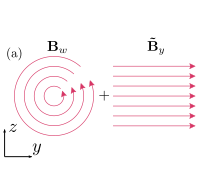
\includegraphics[width=0.8\textwidth]{figs/theory/wires/simplefield.pdf}
    \hfill{}
  \end{subfigure}
  \begin{subfigure}[b]{0.45\textwidth}
    \centering
    \import{figs/theory/wires/}{simpleheat_alone.pgf}
  \end{subfigure} \\
  \begin{subfigure}[b]{0.45\textwidth}
    \centering
    \import{figs/theory/wires/}{simpleheat_y.pgf}
  \end{subfigure}
  \begin{subfigure}[b]{0.45\textwidth}
    \centering
    \import{figs/theory/wires/}{simpleheat_z.pgf}
  \end{subfigure}
  \caption[Two-dimensional wire trap]{
    The field from a simple two-dimensional wire trap. In subfigure (a) a wire carries
    current $I=\SI{1}{\milli\ampere}$ in the positive $x$ direction (out of the
    page) to create the usual field $\mathbf{B}_w$. This is combined with the
    external bias field $\mathbf{\tilde{B}}_y$ to create the two-dimensional trap
    at height $h=\SI{1}{\milli\meter}$
    shown in subfigure (b). The field lines are shown by pink arrows, and the
    magnitude of the resulting field is shown with the blue gradient (darker
    means weaker field, guide to the eye). Cut throughs of the potential are
    shown for $y$ (with $x=0$, $z=h$) in (c) and for $z$ (with $x = y = 0$) in
    (d).
  }
  \label{theory:fig:simplefield}
\end{figure}

Since the field minimum here is a zero, we can approximate the value near the
centre by a (two-dimensional) quadrupole with gradient. The gradient will be
the normal gradient of the wire field at the trap centre
%
\begin{equation}
  B'_w(h) = \left.\frac{\dd B_w}{\dd z}\right|_{z=h} = - \frac{\mu_0 I}{2\pi
      h^2},
\end{equation}
%
where the height can be written in terms of the bias field by
\myeqref{theory:eqn:wire}, and using $B_w(h) = -\tilde{B}_y$
%
\begin{equation}
  h = -\frac{\mu_0 I}{2\pi \tilde{B}_y}.
  \label{theory:eqn:height}
\end{equation}
%
So the gradient near the centre is
%
\begin{equation}
  B' = -\frac{2\pi \tilde{B}_y^2}{\mu_0 I}.
\end{equation}

The depth of the trap is $\mu \tilde{B}_y$, where $\mu$ is the magnetic dipole
moment of the trapped particle. This can be seen in
\mysubfigref{theory:fig:simplefield}{d}: the potential is $B = |B_w(z) +
\tilde{B}_y|$, and so has an asymptote at $B=|\tilde{B}_y|$ as
$z\rightarrow\infty$. It is useful to write this depth as a temperature
%
\begin{equation}
  T  = \frac{\mu \tilde{B}_y}{k_B}.
  \label{theory:eqn:depth}
\end{equation}
%
We can transform such a trap into a Ioffe-Pritchard trap by applying a second
bias field along the $x$ direction to lift the field minimum away from
zero.

Of course, it is commonly desirable to trap in all three dimensions. A simple
way to introduce confinement along the $x$ axis is to introduce a second wire
trap acting in the perpendicular direction. Such a device is called a dimple
trap (or cross conductor trap, or X-trap) and is illustrated in
\myfigref{theory:fig:dimple}. We label the current in the second wire $I_1$
and the new bias field, which is parallel to the $x$-axis and opposes the
$I_1$ field is labelled $\mathbf{B}_x$. In the case that $I_1 \ll I$, the
second wire can be treated as a perturbation of the first. The field minimum is
therefore still at $h$, and its depth is given by \myeqref{theory:eqn:depth}.

\begin{figure}[htb]
    \centering
    \begin{tabular}[t]{cc}
\begin{subfigure}{0.3\textwidth}
    \centering
    \smallskip
    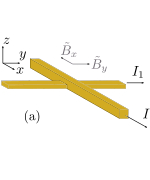
\includegraphics[width=\textwidth]{figs/theory/wires/dimple.pdf}
\end{subfigure}
    &
        \begin{tabular}{c}% if you add [t], than sub images are pushed down
        \smallskip
            \begin{subfigure}[t]{0.4\textwidth}
                \centering
                  \import{figs/theory/wires/}{dimpleheat_alone.pgf}
            \end{subfigure}\\
            \begin{subfigure}[t]{0.4\textwidth}
                \centering
                  \import{figs/theory/wires/}{dimple_x.pgf}
            \end{subfigure}
        \end{tabular}\\
    \end{tabular}
  \caption[Dimple trap]{
    The geometry of the dimple trap is shown in subfigure (a), with the new
    wire along $y$ carrying current $I_1$ intersecting the $I$ wire. An
    additional bias field in the $x$ direction, $\tilde{B}_x$ creates the field
    minimum. The field lines (pink) and magnitude (blue, darker is weaker,
    guide to the eye) is shown in subfigure (b) along $x=0$. Note the strong
    field region along the $y$ axis around the $I_1$ wire. Subfigure (c) shows
    a cut through of the trapping potential in the $x$ direction with $y=0$,
    $z=h$.
  }
  \label{theory:fig:dimple}
\end{figure}

The dimple trap can be used as a quadrupole trap when the bias fields are
chosen to exactly cancel the magnetic field at the centre, or it can be used as
a Ioffe-Pritchard trap when there is a non-zero minimum. We will focus on the
latter case.
%
The trapping frequencies can be obtained as follows. 
%
The trapping from the $I$ wire will be stronger than the $x$-axis
confinement from the $I_1$ wire, hence the trapping frequency in this
direction ($\omega_x$) will be lower than the trapping frequency in the other
directions ($\omega_\perp$). We again write down the field minimum
%
\begin{equation}
  B_0 = \left|\tilde{B}_x + \frac{\mu_0 I_1}{2\pi h}\right|,
\end{equation}
%
the transverse gradient
%
\begin{equation}
  B'_\perp = \frac{\mu_0 I}{2 \pi h^2},
  \label{theory:eqn:dimplegrad}
\end{equation}
%
and the curvature along the weak component
%
\begin{equation}
  B'' = \frac{\mu_0 I_1}{\pi h^3}.
\end{equation}
%
The trap frequencies can be found by comparing to the frequencies of a general
Ioffe-Pritchard trap (see \myeqref{theory:eqn:IP}) and noting that $B'' \ll
B'^2/B_0$. Hence we have in the strong direction
%
\begin{equation}
  \omega_\perp = \sqrt{\frac{\mu B_\perp'^2}{m B_0}},
  \label{theory:eqn:perpfreq}
\end{equation}
%
where $m$ is the particle mass. In the weak direction (along $x$) the frequency
is
%
\begin{equation}
  \omega_x = \sqrt{\frac{\mu B''}{m}}.
  \label{theory:eqn:xfreq}
\end{equation}

It is worth noting that in this simplified diagram, and in those to follow, the
wires are shown as touching. In reality it is common to electrically isolate
the wires from one another during fabrication. However in section~\cm{TODO}, we
will also present a scheme for how electrically connected wires can have their
currents controlled independently.

\subsection{The H-trap}

Consider the dimple trap, but with $\tilde{B}_x$ set to zero. Now what was
previously a magnetic field minimum will be a field maximum. By putting two
such dimple traps next to each other, it is possible to create a local minimum
within which we can trap molecules. Such a trap is called an H-trap, and is
pictured in \myfigref{theory:fig:Htrap}. We label the current due to the second
dimple trap $I_2$, and again note that the bias field in the $x$ direction can
be set to zero. The distance between $I_1$ and $I_2$ is denoted $d$, and we now
refer to the wire carrying current $I$ as the axis of the trap.

\begin{figure}[htb]
  \centering
  \begin{subfigure}[b]{0.4\textwidth}
    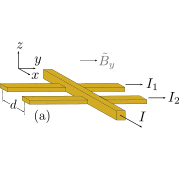
\includegraphics[width=\textwidth]{figs/theory/wires/Htrap.pdf}
    %\vspace{0.1mm}
  \end{subfigure}
  \begin{subfigure}[b]{0.4\textwidth}
    \import{figs/theory/wires/}{Hx.pgf}
  \end{subfigure}
  \caption[H-trap]{The geometry of the H-trap is shown in subfigure (a). In subfigure
  (b) we show the potential for an H-trap with
  $I_1=I_2=I/10=\SI{0.1}{\milli\ampere}$ and $d=\SI{10}{\milli\meter}$. Again the bias field is chosen so
  that $h=\SI{1}{\milli\meter}$.}
  \label{theory:fig:Htrap}
\end{figure}

We note that we need not choose $I_1$ and $I_2$ to be the same, although from
now on we will assume that they have the same magnitude; the sign can differ.
In other words these currents can be parallel or anti-parallel. In the former
case the wires form a Ioffe-Pritchard trap; this is due to the fields from
$I_1$ and $I_2$ adding in the centre, to provide some overall non-zero
component in the $x$ direction. When the currents are anti-parallel, the $I_1$
field opposes the $I_2$ field in the centre of the trap, the two cancel and
there is a field zero. Hence the latter configuration is a quadrupole trap.

In the Ioffe-Pritchard configuration, we can write down the field's
minimum
%
\begin{equation}
  B_0 = \tilde{B}_x + 2\tilde{B}_y \frac{I_1}{I}\frac{h^2}{(d/2)^2 + h^2}
\end{equation}
%
transverse gradient
%
\begin{equation}
  B'_\perp = \frac{2\pi\tilde{B}_y^2}{\mu_0 I}
\end{equation}
%
and curvature~\cite{PhysRevA.79.013407}
%
\begin{equation}
  B'' = \tilde{B}_x + 2\tilde{B}_y\frac{I_1}{I_0}\frac{h^2}{(d/2)^2+h^2}
\end{equation}
%
and the trap frequencies are again given by equations~\ref{theory:eqn:perpfreq}
and~\ref{theory:eqn:xfreq}~\cite{PhysRevA.79.013407}. In the quadrupole
configuration, the trap is characterised by the perpendicular gradient
$B'_\perp$. 

\subsection{Three dimensional single-wire traps}

Although the H-trap provides a method of creating a three dimensional
microtrap, it is not always convenient to have to use three distinct wires.
Fortunately the H-trap can be approximated by a single wire, either in a
U-shape for the quadrupole variant, or a Z-shape for the Ioffe-Pritchard
variant~\cite{2011Ac}. These are pictured in \myfigref{theory:fig:HUZ}. Note
that for the U-trap the currents in the off-axis wires are once again
anti-parallel, and in the Z-trap these currents are parallel. For the U- and
Z-traps, we denote the distance between the end wires as $d$, and refer
to the direction of the current in the central wire as the axis.

\begin{figure}[htbp]
  \centering
  
\includegraphics[width=\textwidth]{figs/theory/wires/HUZcomp.pdf}
  \caption[U- and Z-traps]{Current configuration for U-trap (Z-trap)
  approximating the quadrupole (Ioffe-Pritchard) H-trap configuration.}
  \label{theory:fig:HUZ}
\end{figure}

The Z-trap will be the primary focus of this thesis, and so we will focus on
this as an example. In \myfigref{theory:fig:HZcontours} we compare an H-trap
with a current of \SI{1}{\milli\ampere} on each wire with the potential due to
a single Z-wire also with current \SI{1}{\milli\ampere}. In both cases
$d=\SI{10}{\milli\meter}$, and a bias field of \SI{2}{\milli\gauss} in the $y$
direction is chosen, so as to create a minimum at approximately
$z=\SI{1}{\milli\meter}$ from the axis. The potentials are similarly
comparable for the H-trap in quadrupole configuration and the U-trap. Note that
the ambient magnetic field in the lab can be zeroed by the use of shim coils
outside the experiment.

\begin{figure}[htbp]
  \centering
  \import{figs/theory/wires/}{HZcontours.pgf}
  \caption[Comparison of H- and Z-traps]{
    Contour plots comparing the potentials ($B =
    \sqrt{\mathbf{B}\cdot\mathbf{B}}$) for a H-trap in
    Ioffe-Pritchard configuration (left column) and Z-trap (right column), with
    cut throughs for $z=\SI{1}{\milli\meter}$ (top row) and $x=0$ (bottom row).
    All wires carry a current of $I=\SI{1}{\milli\ampere}$ and a bias field of
    \SI{2}{\milli\gauss} is applied in the $y$ direction.}
  \label{theory:fig:HZcontours}
\end{figure}

This illustrates that a single current-carrying wire can be used to form a trap
in three dimensions. The examples here use length scales of a few millimeters,
and have typical depths of \SI{100}{\nano\kelvin}, but we will discuss in
chapter~\ref{sim} that it is possible to realise much smaller and deeper traps.


\section{Physics of diatomic molecules}
\label{theory:molecules}

Up to this point we have considered abstracted and idealised systems, but in
the next chapter we will begin to think about the realities of trapping cold
molecules on a chip. It is essential that we introduce and understand the
energy structure of diatomic molecules, which is far richer and more complex
than the structure of atoms due to the additional effects of vibration and
rotation of the two nuclei. This section will explain the physics of diatomic
molecules so that the particulars of the cooling transitions and magnetically
trappable states can be easily explained in the next chapter. A more
detailed review of the topic can be found in \inlineref{brown_carrington_2003}.

\subsection{Electronic, vibrational, and rotational energy}

We can begin by considering two atoms, which we label $A$ and $B$,
with masses  $m_i$, $i\in\{A,B\}$ and $m_p$ is the proton rest mass. We say that the location of the
atoms is $\mathbf{R}_i$ and the distance between them is
$R_{AB}$ where $\mathbf{R}_{AB} = \mathbf{R}_B - \mathbf{R}_A$. In the case
that $R_{AB} \rightarrow \infty$ we have two distinct atoms that will behave 
as we would expect them to in isolation (see, for example,
\inlineref{Foot2005}).

As $R_{AB}$ is reduced, the atoms will begin to perturb each other, with the
perturbation dominated by the Coulomb interaction between the various charges.
We can write down the Hamiltonian of such a system, and it is most useful to do
so in the centre of mass (COM) frame, with the reduced mass
%
\begin{equation}
  \mred{} = \frac{m_A m_B}{m_A + m_B}
\end{equation}
%
and COM location
%
\begin{equation}
  \mathbf{R}_\text{COM} = \frac{m_A \mathbf{R}_A + m_B \mathbf{R}_B}{m_A+m_B}.
\end{equation}
%
The Hamiltonian is then the sum of the terms arising from the Coulomb
interaction, and the motion of the molecules
%
\begin{equation}
  H = T_n + T_e + V_{nn} + V_{en} + V_{ee},
\end{equation}
%
where
%
\begin{align}
  T_n &= -\frac{\hbar^2}{2\mred{}}\nabla_{AB}^2,\\
  T_e &= -\frac{\hbar^2}{2 m_e}\sum_{i=1}^{N_e} \nabla_i'^2 -
  \frac{\hbar^2}{2(m_A + m_B)}\sum_{i, j} \nabla'_i \cdot \nabla'_j, \\
  \label{theory:eqn:mpterm}
  V_{nn} &= \frac{Z_A Z_B e^2}{4\pi\epsilon_0 R_{AB}}, \\
  V_{en} &= - \frac{e^2}{4\pi\epsilon_0}\sum_{i=1}^N \left(\frac{Z_A}{R_{Ai}} + \frac{Z_B}{R_{Bi}}\right), \\
  V_{ee} &= \frac{e^2}{4\pi\epsilon_0}\sum_{i<j} \frac{1}{R_{ij}},
\end{align}
%
and we have introduced the relative distances $R_{ij}$ being the distance
between the $i^\text{th}$ and $j^\text{th}$ electrons, and $R_{Ai}$ the
distance between $A$ and the $i^\text{th}$ electron (and similar for $B$) as
shown in \myfigref{theory:fig:mol}.  The total number of electrons is $N_e$.
The primed gradient operators represent differentiation with respect to the COM
coordinates.
%
These terms represent the kinetic energy of the nuclei and the elctrons
in the COM frame ($T_n$ and first term in $T_e$ respectively), the various
Coulomb attraction and repulsions $V_*$ terms), and the
so-called mass polarisation term. This is the second term in
\myeqref{theory:eqn:mpterm}, and it is a correction term to account for small
fluctuations in the COM. This is necessary since the movement of any one
particle will change the position of the COM, hence the particle coordinates
are all coupled in this frame. Fortunately this term can usually be neglected,
or treated as a perturbation~\cite{brown_carrington_2003, modestrue}.
%
The time-independent Schr\"odinger equation (TISE),
%
\begin{equation}
  H\psi = E\psi
\end{equation}
%
can now in principle be solved for this Hamiltonian, although we will only
sketch the solution here. A full derivation can be found in
\inlineref{brown_carrington_2003}.

\begin{figure}
  \centering
  \includegraphics[width=0.25\textwidth]{figs/theory/mols.pdf}
  \caption[Geometry of a diatomic molecule]{
    The geometery of a diatomic molecule, with relevant vectors labelled.
    Nuclei in blue and pink, electrons in purple.
  }
  \label{theory:fig:mol}
\end{figure}


\subsubsection{Electronic states}

The wavefunction
$\psi$ is a function of $\mathbf{R}_{AB}$ and the position of each of the
electrons, that is
%
\begin{equation}
  \psi = \psi(\mathbf{R}_{AB}, \mathbf{R}_1, \dots \mathbf{R}_{N_e}).
\end{equation}
%
We now make the Born-Oppenheimer approximation, where we say that because the
nuclear mass is much higher than that of the electrons, the nuclei are
stationary on the timescale of the electronic motion. For this
reason we are able to separate the wavefunction into the electronic and nuclear
parts
%
\begin{equation}
  \psi(\mathbf{R}_{AB}, \mathbf{r}) = \psi_e(\mathbf{R}_{AB}; \mathbf{r})
  \psi_n(\mathbf{R}_{AB}).
\end{equation}
%
Note here that $\mathbf{R}_{AB}$ is treated as a parameter of $\psi_e$ and we
have introduced $\mathbf{r} = \{\mathbf{R}_1, \dots \mathbf{R}_{N_e} \}$ to
represent the set of electronic coordinates.

There is then a separate electronic TISE
%
\begin{equation}
  H_e \psi_e(\mathbf{R}_{AB}; \mathbf{r}) = E_e(R_{AB}, \mathbf{r})\psi_e(\mathbf{R}_{AB};
  \mathbf{r}),
  \label{theory:eqn:TISEelectron}
\end{equation}
%
where the Hamiltonian $H_e = H - T_n$ is the previous Hamiltonian but excluding
the term for the nuclear motion.
%
This problem now begins to resemble the analogous one of finding the electronic
states of atoms, and can be solved by similar numerical methods~\cite{Foot2005,
bransden2003}. The upshot is that it is possible to determine the electron
eigenstates, which we label $\psi_e(\mathbf{R}_{AB}; q)$, with $q$ being the
quantum number for the electronic configuration\footnote{The numbering of the
electronic configurations is actually more complicated than this. We will
discuss how these states are labelled in section~\ref{theory:qnos}.}. The
energy of the state is now denoted $E_e(q; R_{AB})$, with $q$ as a parameter
and $E_e$ a function of  $R_{AB}$.  It is common to approximate this energy as
the Morse potential
%
\begin{equation}
  E_e(q; R_{AB}) = D(1-e^{-\beta(R_{AB} - R_{AB}^0)})^2,
\end{equation}
%
where $R_{AB}^0$ is the equilibrium displacement of the nuclei, $D$ is the
dissociation energy, and $\beta$ is a parameter for the width of the
potential. All of these are dependent on the electronic configuration, but this
dependence is suppressed in the notation. From here on, we suppress the
dependence of $E_e$ on $R_{AB}$ and write $E_e(q; R_{AB}) = E_e(q)$.

Implicit in the Born-Oppenheimer approximation is that the electronic
configuration is the largest contribution to the state's energy. We can make a
naive estimate of this energy as the typical kinetic energy of the electrons
%
\begin{equation}
  E_e \approx \frac{p^2}{2m_e} = \frac{\hbar^2}{2m_e a^2},
\end{equation}
%
where $a\sim\SI{1}{\angstrom}$ is the length scale of the molecule and $m_e$ is
the electron mass, so that $E_e/h \sim \SI{1000}{\tera\hertz}$. This
gives us the first order contribution to the energy of the molecule. 

\subsubsection{Nuclear motion}

We now turn our attention to the nuclear wavefunction. It is possible to
continue manipulation of the Hamiltonian so as to write down the relevant
TISE for the nuclei~\cite{brown_carrington_2003}
%
\begin{equation}
  \left(-\frac{\hbar^2}{2\mred{}}\nabla_{AB}^2 + E_e(q; R_{AB}) -
  E\right)\psi_n(\mathbf{R}_{AB}) = 0.
  \label{theory:eqn:nucTISE}
\end{equation}
%
Note that the potential that the nuclei move through is the potential
generated by the electron configuration, and that this potential is central. We
can therefore anticipate the separation of the nuclear wavefunction into radial
and angular parts,
%
\begin{equation}
  \psi_n(\mathbf{R}_{AB}) = \frac{1}{R_{AB}}f(R_{AB})Y_{R, m_R}(\theta, \phi),
  \label{theory:eqn:nucsep}
\end{equation}
%
where we choose the factor of $1/R_{AB}$ to simplify the equation in the rest
of the section. We will introduce the operator $\mathbf{R}$ to describe the
rotational angular momentum. The angular part of the solution is given by the usual
spherical harmonics $Y_{R, m_R}$ where
%
\begin{align}
  \mathbf{R}^2 Y_{R, m_R} &= R(R+1) Y_{R, m_R}, \\
  R_z Y_{R, m_R} &= m_R Y_{R, m_R}.
\end{align}
%
The rotational quantum number for the state, and $m_R$ is the projection onto
the axis.

Substitution of \myeqref{theory:eqn:nucsep} into \myeqref{theory:eqn:nucTISE}
yields 
%
\begin{equation}
  \left(-\frac{\hbar^2}{2\mred{}}\frac{\dd^2}{\dd R_{AB}^2} +
    \frac{\hbar^2 R(R+1)}{2\mred{}R_{AB}^2} + E_e(q; R_{AB}) - E\right)f(R_{AB}).
\end{equation}
%
where we have expanded $\nabla_{AB}^2$ in terms of the second derivative in
$R_{AB}$ and the angular momentum operator $\mathbf{R}^2$. This equation is now
that of an oscillator in the Morse potential $E_e(q; R_{AB})$, with an
additional energy term that arises due to the rotation,
%
\begin{equation}
  E_\text{rot}(R) = \frac{R(R+1)}{2\mred{} (R_{AB}^0)^2}.
  \label{theory:eqn:rotenergy}
\end{equation}
%
Here we have approximated the internuclear separation to be at its equilibrium
value.

The vibrational part of the wavefunction can be solved by the standard
computational methods for finding the wavefunctions of anharmonic
potentials~\cite{Foot2005}. These vibrational states form a ladder of
states inside an anharmonic potential~\cite{Binney} as pictured in
\myfigref{theory:fig:vibtrans}. We label these states with the quantum number
$v$, and so re-write $f(R_{AB}) = f_v(R_{AB})$ to clarify which vibrational
level we are referring to.

At low energy the Morse potential approximates
to a harmonic potential
%
\begin{equation}
  E_e(q; R_{AB}) \approx D\beta^2(R_{AB} - R_{AB}^0)^2,
\end{equation}
%
where the vibrational frequency is related to the potential by
%
\begin{equation}
  \frac{1}{2}\mred{}\omega_\text{vib}^2(R_{AB}-R_{AB}^0)^2 = D\beta^2(R_{AB}-R_{AB}^0)^2.
  \label{theory:eqn:vibfreqrel}
\end{equation}  
%
We can estimate this vibrational frequency by considering the opposite limit,
near dissociation. We approximate $D$ to be the typical electronic energy $E_e$
and note that for dissociation to occur we expect $\beta(R_{AB} - R_{AB}^0) >
1$ and also that at this point $(R_{AB} - R_{AB}^0)^2\sim a^2$. We therefore
substitute into \myeqref{theory:eqn:vibfreqrel} $D\approx E_e$ and
$\beta\approx a^{-1}$
%
\begin{equation}
  \hbar\omega_\text{vib} \approx \sqrt{\frac{\hbar^4}{\mred{} m_e a^4}} \sim
    h\times\SI{10}{\tera\hertz},
\end{equation}
%
where we took $\mred{}\approx m_p$. The vibrational energy $E_\text{vib}$ can
be approximated for low $v$ as a harmonic oscillator, so that
%
\begin{equation}
  E_\text{vib}(v)\approx \hbar\omega_\text{vib}\left(v+\frac{1}{2}\right).
\end{equation}

We now have and estimate for the vibrational energy, and the final step is to
compare this to the rotational energy in \myeqref{theory:eqn:rotenergy}, where
we expect typical values
%
\begin{equation}
  E_\text{rot}(0) = \frac{\hbar}{2 \mred{} R^0_{AB}} \sim h\times\SI{100}{\giga\hertz}
\end{equation}
%
it is clear that the rotational energy levels can be treated as perturbations
of the vibrational levels.

\subsubsection{Qualitative summary}

We have described how the wavefunction of a diatomic molecule in free space can
be written as three separate wavefunctions, one each for the electronic,
vibrational and rotational Hamiltonians. We denote the wavefunction in the form
%
\begin{equation}
  \psi_{q, v, R, m_R} = \frac{1}{R_{AB}}\psi_e(\mathbf{R}_{AB};q)
  f_v(R_{AB})Y_{R, m_R}(\theta, \phi).
\end{equation}
%
The Born-Oppenheimer approximation states that the electrons move on a much
faster timescale than the nuclei, and hence have a higher energy (by about a
factor of $100$) than the nuclear motional energy.

Due to this difference in timescale, the nuclei move in the electrostatic potential
generated by the electrons, which can be approximated to be a Morse potential. This
means that the nuclei vibrate as an anharmonic oscillator, with some
equilibrium distance $R_{AB}^0$. The vibrational motion is again higher (by
about a factor of $100$) than the rotational energy, which comes from the
tumbling of the two nuclei. The total energy is
%
\begin{equation}
  E_{q,v,R} = E_e(q) + E_\text{vib}(v) + E_\text{rot}(R).
\end{equation}


\subsection{Transitions}
\label{theory:transitions}

% Just basic ideas or electronic, vibrational, ro-vibrational transitions.
% Talk more about microwave spectroscopy elsewhere?

We will now state the selection rules describing the allowed transitions
between the various states of the molecule~\cite{brown_carrington_2003}. We
will label the original state in the transition $\ket{g} = \ket{q, v, R, m_R}$
and the final state $\ket{e} = \ket{q', v', R', m_R'}$.
%
It is useful to remember that the following results are found by considering
the intensity of the transition. This, as we saw above when discussing the Rabi
frequency, is proportional to $|d_{ge}|^2$, where
%
\begin{equation}
  d_{ge} = \bra{g}\mathbf{d}\cdot\bm{\epsilon}\ket{e}
\end{equation}
%
is the matrix element of the transition. Again we have $\mathbf{d}$ as the
dipole moment operator, and $\bm{\epsilon}$ as the unit vector representing the
polarisation of the light.

This matrix element is best evaluated by re-writing it in a spherical basis,
then writing this basis so that the $z$ axis is aligned with the internuclear
axis. This yields an integral over the electronic, vibrational and rotational
wavefunctions. Deriving this integral and its solution is beyond the scope of
this discussion, as it is not required to understand the rest of the thesis. It
has been explained eloquently and succinctly in various texts, including
\inlineref{brown_carrington_2003}.

\subsubsection{Pure rotational transitions}

\jvg{How is the rotation axis aligned?}
\cm{Need to insert something somewhere about this -- it relates to the point I
  am missing about the dipole moments alignment that was the main sticking
  point in the viva -- should talk to Mike.}

In a pure rotational transition, the electronic and vibrational states are
unchanged ($q'=q$ and $v'=v$). Such transitions are permitted only when $\Delta
R = R' - R = \pm1$. The selection rule for $m_R$ is dependent on the
polarisation of the light. For linearly polarised light $\Delta m_R = m_R' -
m_R = 0$, whereas for circularly polarised light $\Delta m_R =  \pm1$ for
$\sigma^\pm$ polarised light. The molecule tumbles with a rotation vector
perpendicular to the internuclear axis, any rotation around the internuclear
axis is symetrically invariant.

\subsubsection{Vibrational transitions}

In the case where there is still no change in electronic state ($q'=q$) we have
the same selection rules for any change in the rotational quantum numbers. It
can be shown that when the states are well approximated by a quantum harmonic
oscillator (which occurs for sufficiently small $v$ so that we can ignore the
anharmonicity), the additional selection rule for the vibrational transition is
$\Delta v = v' - v = \pm 1$. Of course, $\Delta v = 0$ is allowed, but then
this reduces to the above case of a pure rotational transition.

\subsubsection{Changing the electronic state}

When the electronic state changes the analysis is more complicated, and there
are no consistent selection rules for the change in the vibrational state. This
can be explained when we recall that the matrix element $d_{ge}$ is an integral
over the state's wavefunction $\psi = R_{AB}^{-1}\psi_ef_v(R_{AB}) Y_{R, m_R}$.
When the electronic states are the same, the electronic contribution becomes a
factor of one and the vibrational states are all states from the same
anharmonic oscillator, as can be seen in \myfigref{theory:fig:vibtrans}. In
this case we can derive the above selection rules.

% For reference, in this fig, the functions are two gaussians and
% (x**5-18*x**3+15*x)*exp(-x**2)
\begin{figure}
  \centering
  \includegraphics[height=0.4\textwidth]{figs/theory/vibtrans.pdf}
  \caption[An electronic transition in a diatomic molecule]{
    A cartoon depiction of a transition between electronic states. Various
    vibrational wavefunctions (blue) are shown for two electronic potentials.
    The $0\rightarrow0$ transition is weak, since there is small overlap
    between the vibrational wavefunctions, but the $0\rightarrow4$ transition
    (dashed line) is stronger.
  }
  \label{theory:fig:vibtrans}
\end{figure}

Now that $q\neq q'$, the vibrational states are not states of the same
potential, and so the overlap integral of the wave functions must
be computed numerically. The vibrational component of this integral is called
the Franck-Condon factor, and is written as
%
\begin{equation}
  q_{v',v} = \left|\int f^*_{v'}(R_{AB})f_v(R_{AB})\dd R_{AB}\right|^2.
\end{equation}
%
The rotational state can change by the same selection rules as before, except
in the case that the rotational angular momentum is coupled to the angular
momentum of the electrons. In this case we can have $J$ as the good quantum
number, with a selection rule $\Delta J = 0, \pm1$.

\subsubsection{Parity}

Since $\mathbf{d}$ is anti-symmetric under parity inversion, $d_{ge}$ will be
zero unless the parity of the wavefunction changes during the transition. This
does not apply to homonuclear molecules. 

\subsection{Good quantum numbers}
\label{theory:qnos}

We will now briefly review the quantum numbers that we have introduced to
describe the molecule state. First note that the quantum number for the
electronic level is not really a quantum number at all. It obfuscates the true
quantum numbers, which come from the angular momentum operators for the
electrons. We will describe the good quantum numbers for two of Hund's
cases~\cite{brown_carrington_2003}, which differ depending on how strongly each
of the angular momentum operators couple to each other. They are pictured in
\myfigref{theory:fig:hund}.

\begin{figure}
  \centering
  \includegraphics[width=0.8\textwidth]{figs/theory/hund2.pdf}
  \caption[Hund's cases]{
    Coupling schemes in Hund's (a) and (b) cases. Arrows are angular
    momenta. Dashed circles indicate precession of the angular momenta about
    various axes. See main text for detailed description. This figure is
    adapted from \inlineref{brown_carrington_2003}.
  }
  \label{theory:fig:hund}
\end{figure}


In the first case (a), the electron orbital angular momentum $\mathbf{L}$ is
strongly coupled to the molecular axis by the electrostatic force, and the spin
angular momentum $\mathbf{S}$ couples strongly to $\mathbf{L}$ by spin-orbit
coupling. Hence, these momenta both precess around the molecular axis. The good
quantum numbers associated with these operators are their projections onto the
axis which we label $\Lambda$ and $\Sigma$  respectively, as well as $S$. $L$
is not a good quantum number since it couples very strongly to the axis and so
precesses rapidly around it.
%
The rotation operator $\mathbf{R}$ coupling is much weaker, and hence can be
approximated to couple to the projection of $\mathbf{L} + \mathbf{S}$ onto the
axis. We label this projection $\mathbf{\Omega} = \Omega \mathbf{\hat{e}}$
where $\mathbf{\hat{e}}$ is the unit vector along the internuclear axis, and $\Omega =
\Lambda + \Sigma$. The total angular momentum is $\mathbf{J} = \mathbf{L} +
\mathbf{S} + \mathbf{R}$. Again, due to the rapid precession of $\mathbf{L}$
and $\mathbf{S}$, we show this in the figure as a precession of
$\mathbf{\Omega}$ and $\mathbf{R}$ around $\mathbf{J}$. Note that
$\mathbf{\Omega}$ is not truly an operator, and is only useful for illustrative
purposes.

In the second case of interest (b), $\mathbf{L}$ is strongly coupled to the
axis as before, and its projection onto the axis is quantum $\Lambda$. $L$ is
not a good number for the same reason as before.  $\mathbf{R}$ has the next
strongest coupling, so we define a new operator $\mathbf{N} = \mathbf{L} +
\mathbf{R}$, which for illustrative purposes we show in the figure as $\Lambda
\mathbf{\hat{e}} + \mathbf{R}$. Finally $\mathbf{N}$ and $\mathbf{S}$ add
together to form a new total angular momentum $\mathbf{J} = \mathbf{N} +
\mathbf{S}$. If $L=0$ then the state will belong to this coupling scheme. The
good quantum numbers for both cases are summarised in the figure. 

We label the electronic states by spectroscopic notation taking the form
%
\begin{equation*} 
  \text{(Unique letter)}^{2S+1}|\Lambda|^\pm_{|\Omega|},
\end{equation*}
%
where the unique letter is always $X$ for the ground state, and for the excited
states are 
incrementing letters of the alphabet, starting with $A$ for the first
excited state. $\Lambda$ is not represented by its numerical value, but
by the Greek characters $\Sigma$, $\Pi$, $\Delta$, etc.\ in analogy with the
notation for the orbital states in atoms. The superscript $\pm$ represents the
is only used for $\Sigma$ states, and is defined by the change to
the wavefunction on reflection through a plane containing the nuclear axis.
When $\Omega$ is redundant it can be omitted.

Up to this point we have mainly denoted the wavefunctions as functions, but we
will soon find it useful to write the states using braket notation. We will not
denote electronic states, this way, but will describe the other quantum
numbers. For example, we may write for a Hund (b) case state $\ket{N, S, J,
\Lambda}$. However, for an electronic state where $L=0$, we could express this
in an equivalent manner such as $\ket{N, m_N}\ket{S, m_S}$. The
quantum number that the ket refers to is implicit by its contents.

\subsection{Hyperfine structure}

The rotational states can be further split into hyperfine states by the angular
momentum contribution of the nuclear spin, which has operator $\mathbf{I}$. The
new total angular momentum is  $\mathbf{F} = \mathbf{J} + \mathbf{I}$. These
states will be important later, since the $m_F$ substates will be used as
weak-field seekers for magnetic trapping.

\subsection{Cooling and trapping molecules}
\label{theory:coolmols}

Up to this point we have discussed only the theoretical descriptions of cooling
for two-level systems. Although useful, and good descriptions of atomic
systems, schemes for cooling and trapping molecules are somewhat more involved.
They will be described in greater detail in the context of the \CaF{}
experiment in the next chapter, but here I outline the key differences from the
two-level systems discussed in section~\ref{theory:cooltrap}.

\textbf{Vibrational repumping:} Consider a three-level system, with two ground
states $\ket{g_0}$ and $\ket{g_1}$ and excited state $\ket{e}$. If we implement
a two-level cooling scheme between $\ket{g_0}$ and $\ket{e}$ then this may well
reduce the particle's temperature. However if the particle can decay from
$\ket{e}$ into $\ket{g_1}$, then this particle can become dark to the cooling
laser. This can occur for diatomic molecules, for example if the molecule
decays from the excited electronic state into a ground electronic state with
higher vibrational energy. In such cases it is necessary to introduce
additional lasers which will repump these dark states, and ensure that the
particle is not lost from the cooling cycle.

\textbf{Rotational branching:} Similar decays into dark states can occur by
rotational branching. One way to avoid this is to drive cooling transitions on
states with rotational quantum numbers $N=1 \rightarrow N'=0$. Then by the
selection rules given in section~\ref{theory:transitions} ($\Delta R =  \pm1$
and parity), it is not possible for a particle in the excited state to decay
into states with other values of $R$. This is explained further in
\inlineref{Fitch2021}.

\textbf{Destabilising dark states:} We will see in section~\ref{overview:MOT}
that the complex structure of the molecule means that a type-II MOT is required
for trapping. This will provide weaker confinement than the type-I MOT
described above, but is required in order to address ground states that would
otherwise be dark to the cooling light.


\chapter{Overview of the experiment}
\label{overview}
The design of the \CaF{} chip experiment was motivated by three main factors:
the need to integrate with the existing experiment, the core proposal of
confining molecules close to a microwave guide, and the practicalities of
fabricating the chip. In this chapter I will describe how the first two factors
informed the design choices, with changes due to fabrication discussed in
chapter~\ref{fab}. The design will be further justified by simulation in
chapter~\ref{sim}.
%
We begin with a discussion of the existing experiment, which will be used to
create the ultracold \CaF{} for loading onto the chip. I will then give an
overview and motivation of the design of the chip experiment.


\section{Existing \CaF{} experiment}
\label{overview:existing}

In this section I will present a summary of the process used to produce
ultracold \CaF{} molecules in a magnetic trap, which we intend to load onto the
chip trap. We will consider the various stages of the process, which are
presented in \myfigref{overview:fig:CaFcartoon}. First a beam of \CaF{}
molecules is created using a buffer gas source~\cite{Truppe2018}. A fraction of
the molecules in the beam are slowed to below the capture velocity of the MOT
by radiation pressure from counter-propagating resonant
light~\cite{Truppe2017a}. We can also apply separate light in the transverse direction
to improve collimation of the beam during its flight.
The molecules are captured in a MOT~\cite{Williams2017} and cooled in optical
molasses~\cite{Truppe2017} before being optically pumped into a weak field
seeking state~\cite{WilliamsMagnetic2018}. This allows for magnetic trapping
and transport of the molecules. The experiment is conducted under ultra-high
vacuum (UHV, $P<\SI{1E-9}{\milli\bar}$) conditions to limit background induced
loss. Only the source chamber operates at a higher pressure, but the molecule
beam quickly exits this chamber into the low pressure region. 

\begin{figure}
  \centering
  \includegraphics[width=0.8\textwidth]{figs/overview/cartoon.pdf}
    %\begin{overpic}[width=0.8\textwidth]{figs/overview/cartoon_notext.pdf}
    %  \put(5, -1){Source}
    %  \put(32, -1){Slowing}
    %  \put(70.5, -1){MOT}
    %  \put(78, 55){\color{pink}{To chip}}
    %  \put(36, 52){\color{Lorange}{\pewpew{}{00} and repumps}}
    %  \put(95, 29){\color{Lgreen}{\pewpew{S}{00}}}
    %\end{overpic}
    %\vspace{1cm}
  \caption[\CaF{} source]{
    A schematic of the \CaF{} source, slowing region and MOT chamber.  \CaF{}
    molecules (blue) are produced by the buffer gas cell, and are slowed by
    longitudinal slowing and transverse cooling light (green, \pewpew{S}{00}).
    The molecules are then captured in a MOT (MOT light \pewpew{}{00} and
    repumps combined are shown here in orange) where they can be further cooled
    and transferred to a magnetic trap. The molecules can then be transported
    out of the chamber by the MTT in the direction of the pink arrow. A
    detailed view of the source is shown in \myfigref{overview:fig:source}. This
    figure is based on one in \inlineref{Truppe2017}.}
  \label{overview:fig:CaFcartoon}
\end{figure}

\subsection{\CaF{} energy structure and constants}

The energy structure of \CaF{} is depicted in
\myfigref{overview:fig:CaFenergy}. Here we show only the levels that are
pertinent to this thesis, those being the X, A and B electronic levels up to
vibrational level $v=3$, 2 and 0 respectively. The relevant Hund's cases are
(b), (a) and (b) respectively. For the X state, we will discuss $N=$
\numrange{0}{2} but for clarity $N=2$ is not included in this figure.
%
Figure~\ref{overview:fig:CaFenergy} and \mytableref{overview:table:lasers} also
label the various lasers that are used to addressed the \CaF{} transitions. We
denote these \pewpew{}{vv'} where $v$ ($v'$) is the lower (excited)
vibrational level that the laser addresses. The superscript $S$ is used to
distinguish the $X\rightarrow B$ transition since it is used for the slowing
light.

\begin{figure}
  \centering
  \includegraphics[width=0.98\textwidth]{figs/energylevels/main_sbs_3.pdf}
  \caption[The energy levels of \CaF{}]{
    The energy levels of \CaF{} are shown, along with the lasers that will be
    used to address the various transitions (further information is found in
    \mytableref{overview:table:lasers}). The branching ratios for the allowed
    decays are shown with dashed lines. Note that the $X(N=0)$ level is
    included, but for simplicity the $X(N=2)$ level is omitted. The box shows
    the hyperfine states of $X(N=1, v=0)$, how these arise from the $N$ and
    $J$ angular momenta is described in the main text. This figure is adapted
    from \inlineref{Williams2017}. 
  }
  \label{overview:fig:CaFenergy}
\end{figure}

\begin{table}
  \centering
\begin{tabular}{llll}
  \hline\hline
  Symbol & Ground state & Excited state & Wavelength (\si{\nano\meter}) \\
  \hline
  \pewpew{}{00} & $X(v=0)$ & $A(v=0)$ &  606.3 \\
  \pewpew{S}{00} & $X(v=0)$ & $B(v=0)$ & 531.0 \\
  \pewpew{}{01} & $X(v=0)$ & $A(v=1)$ & 628.6 \\
  \pewpew{}{12} & $X(v=1)$ & $A(v=2)$ & 628.1 \\
  \pewpew{}{23} & $X(v=2)$ & $A(v=3)$ & 628.7 \\
  \pewpew{}{10} & $X(v=1)$ & $A(v=0)$ & 585.4 \\
 \hline
\end{tabular}
\caption[Lasers, transitions and wavelengths]{
  The various lasers used in this thesis.  The laser \pewpew{}{10}
  is included for completion, and will be explained in
  chapter~\ref{exper}.
  }
  \label{overview:table:lasers}
\end{table}

The permitted decay paths are shown by the dashed lines, along with their
branching ratios. One of the reasons \CaF{} is chosen for study over other
molecules is its highly diagonal Franck-Condon factors, so that most decays
occur with $v'=v$. However, as we discussed in section~\ref{theory:coolmols},
for large numbers of scattered photons we must employ the various repump lasers
to avoid pumping into states that are dark to the cooling light. This will be
discussed further when describing slowing of the beam and the MOT.

Hyperfine splitting occurs in \CaF{} due to the spin-half contribution of the
fluorine atom. This is not resolved in the $A$ state, but it accounts for the
hyperfine splitting of the $X$ state as is shown in the box of
\myfigref{overview:fig:CaFenergy}. It is worth explaining why we have the four
$F$ states $F=2,1^+,0,1^-$. These arise due to the combination  of the
hyperfine interaction and a spin rotation interaction of the form
$\mathbf{S}\cdot\mathbf{N}$. Since we are in Hund's (b) case, the $N=1$ state
is split into angular momenta states $\mathbf{J}= \mathbf{N} + \mathbf{S}$.
Here $S=1/2$, so the possible values of $J$ are $N+1/2$ and $N-1/2$ (with the
exception of $N=0$ where we have only $J=1/2$). For $N=1$, we have $J=3/2$ and
$J=1/2$. Each of these is again split by the hyperfine interaction into
$\mathbf{F} = \mathbf{J} + \mathbf{I}$, with $I=1/2$. This gives us the allowed
values $F=2,1^+,0,1^-$.

In the $B$ state, the $F=0$ and $F=1$ states are split by \SI{20}{\mega\hertz},
which can usually be neglected for the purposes of our discussion. A full
description of the \CaF{} energy structure and various constants can be found
in \inlineref{Anderegg2019a}, those that are most useful are presented in
\mytableref{overview:table:constants}.

\begin{table}
  \centering
\begin{tabular}{lll}
  \hline\hline
  Constant & Symbol & Value \\
  \hline
  Mass & m & \SI{59}{\amu}\\
  Electric dipole moment ($X$ state) & $\mu_e$ & $\SI{-3.08}{\debye}$\\
  % Don't confuse EDM with transition moment
  Magnetic dipole moment & $g_F\mu_B m_F$ & \\
  % This is what Ed uses in his notebook, I think it is the same as mu_e...
  % Had to convert form his units, but pretty sure this is right.
  %Chemistry dipole moment & $\mu_c$ & $3\si{\debye}$ \\
 \hline
\end{tabular}
\caption[\CaF{} constants]{
  Various constants for \CaF{} taken from \inlineref{Anderegg2019a}. Note that
  the magnetic dipole moment is given in terms of the g-Factor $g_F$ and the
  quantum number $m_F$, which are state dependent, as well as the Bohr magneton
  $\mu_B = \SI{9.274}{\joule\per\tesla}$.
  \jvg{How does this compare to cavity QED system?}
  \cm{I have a comment here 'Don't confuse EDM with transition moment' I think
    there is some fundamental misunderstanding here and I need to talk to Mike
    about it.}
  }
  \label{overview:table:constants}
\end{table}

\subsection{Buffer gas source}

We begin all our experiments by creating a pulsed beam of \CaF{} molecules
using a buffer gas source. This is pictured in \myfigref{overview:fig:source}
and consists of a copper cell which is cryogenically cooled to \SI{4}{\kelvin}.
%
Helium gas, also cooled to \SI{4}{\kelvin}, and \SFsix{} gas near room
temperature, flow through the cell. A \Ca{} target (shown in blue) is ablated
by a pulsed Nd:YAG laser. The \Ca{} reacts with the \SFsix{} to produce \CaF{}, which is
then flushed out of the cell by the helium flow.

\begin{figure}
  \centering
  \includegraphics[width=0.6\textwidth]{figs/overview/cell.pdf}
  \caption[The buffer gas cell]{
    The buffer gas cell. Helium and \SFsix flow into the cell. \Ca{}
  atoms are ablated from a target (shown in blue) by a Nd:YAG laser. \CaF{} molecules are
formed which thermalise with the \He{} and a molecule beam exits from the aperture.}
  \label{overview:fig:source}
\end{figure}

The cell is designed to optimise the flow of \He{} so as to entrain the 
\CaF{} and guide it to the exit aperture without the creation of vortices,
where the molecules can be trapped~\cite{Truppe2018}. For this reason \He{}
enters from towards the rear of the cell at \SI{4}{\kelvin} and flows towards
the exit aperture.  The \Ca{} target is  mounted on a rotating stage, so that
when one region is depleted another can be targeted.

In order to prevent excess helium entering the slowing and MOT chambers, a
second aperture is positioned between the source and slowing chambers.
Differential pumping ensures that the slowing chamber remains at UHV. A
mechanical shutter at this aperture reduces the time that helium is able to
leave the source chamber to only the time when there is a pulse of \CaF{}. We
also use a copper shield, coated with coconut charcoal and cooled to
\SI{4}{\kelvin} as a helium absorber~\cite{doi:10.1116/1.574141}. This is
thermally cycled overnight when the source is not in use to avoid saturation.
As noted in \inlineref{Jurgilas2021}, this buffer gas source originally
produced up to \SI{5E10}{molecules/steradian} molecules in $X(N=1, v=0)$ per
pulse, with a
mean velocity of \SI{160}{\meter\per\second}~\cite{Truppe2018} but its
performance has degraded since the original report. As a result we now observe
\SIrange{50}{60}{\percent} lower MOT population than at the time
\inlineref{Williams2017} was published.

\subsection{Slowing the beam}

The buffer gas source produces a beam of molecules with mean forward velocity
\SI{160}{\meter\per\second} -- slower than for example, a supersonic
source~\cite{Mathavan2016} but they are still far above the capture velocity of
our MOT, which is approximately \SI{10}{\meter\per\second}. The beam's velocity
can be further reduced by radiation pressure due to a counter-propagating beam
of \pewpew{S}{00} slowing light. This is chirped to account for the change in
Doppler shift of the transition frequency as the molecules slow. The slowing
light is also combined with the \pewpew{}{10} repump light to avoid pumping
into the $X(v=1)$ state. To again account for Doppler shift during slowing, the
repump light is frequency broadened by \SI{300}{\mega\hertz} by a series of
three elecro-optic modulators.

% Time and final velocity according to Hannah's thesis
We apply the light for \SI{6}{\milli\second}, which slows over approximately
\SI{90}{\centi\meter} of travel from the buffer gas cell's exit aperture.
Linear chirps used in previous experiments have been used to slow the molecules
for loading into the MOT, as detailed in \inlineref{Williams2017}. Implementing an
exponential chirp originally proposed in \inlineref{Anderegg2019}  produced a
\SIrange{60}{80}{\percent} improvement in the number of molecules in the
MOT~\cite{Jurgilas2021}.

It is also possible to reduce the transverse velocity of the beam by applying
slowing beams in the perpendicular direction close to the source. This is shown
for one dimension in the `slowing and transverse cooling' section of
\myfigref{overview:fig:CaFcartoon}, however in reality there is a second pair
of beams going into and out of the page. For this cooling step we also use the
$X\rightarrow B$ transition along with the \pewpew{}{10}
repump~\cite{Jurgilas2021}.

\subsection{Capture in a MOT}
\label{overview:MOT}

We aim to capture molecules in a MOT positioned \SI{130}{\centi\meter} from the
cell's exit aperture inside a separate vacuum chamber. The MOT magnetic field
is provided by in-vacuum anti-Helmholtz coils and the MOT light is formed from
a single beam which is reflected along each axis before being retro-reflected
through the entire experiment to provide the restoring beams.
%
We described in section~\ref{theory:coolmols} that laser cooling and trapping of diatomic
molecules requires us to address three key differences to atomic systems. The
first is the repumping of the vibational levels. We apply vibrational repumps (\pewpew{}{10}, \pewpew{}{21}
and \pewpew{}{32}) along with the main cooling light (\pewpew{}{00}).  All of these beams must have the r.f.\ sidebands
to address the hyperfine levels of the $X$ state (recall that the hyperfine
levels of $A$ are unresolved).

The second nuance is the rotational branching, which we avoid by cooling on the
$X(N=1) \rightarrow A(N=0)$ transition. This immediately leads to the third
nuance, which is the remixing of resulting dark states. 
%
The \CaF{} MOT is a type-II MOT~\cite{1367-2630-18-12-123017}, meaning that the
angular momentum of the excited state  is less than that of the ground state .
Unlike a type-I MOT (where $F'>F$), it is possible for a molecule that has been
pumped into the excited state to decay into a dark state, or into a state that
is anti-trapped by the MOT~\cite{Fitch2021}.
%
To resolve this, we employ a dual-frequency MOT.
\myfigureref{overview:fig:dualfreq} illustrates this MOT scheme for the
simplified case of a ground state with $F=1$ and an excited state with $F'=0$.
%
When there is no blue-detuned light, any molecule that decays into the $m_F=-1$
state can be lost from the cycle. When blue-detuned light of opposite
polarisation is present these molecules can be repumped. 

\begin{figure}
  \centering
    \begin{overpic}[abs, width=0.2\textwidth]{figs/overview/typeII.pdf}
      \put(-40, 43){$F=1$}
      \put(-40, 148){$F'=0$}
      \put(90, 43){$m_F=0$}
      \put(90, 81){$m_F=1$}
      \put(90, 5){$m_F=-1$}
      \put(5, 5){\color{blue}{$\sigma^+$}}
      \put(5, 81){\color{pink}{$\sigma^-$}}
    \end{overpic}
  \caption[Dual-frequency cooling scheme]{
    A dual frequency scheme for the type-II case $F'=0$, $F=1$. The molecules
    in each state (circles) can be pumped by their corresponding red- (blue-)
    detuned light. This figure is adapted from one in \inlineref{Williams2018}.
  }
  \label{overview:fig:dualfreq}
\end{figure}

We are typically able to capture on the order of $10^4$ molecules from our
beam.  The MOT population can be estimated by the light-induced fluorescence.
The MOT temperature is reduced to its minimum value by lowering the intensity
of \pewpew{}{00}, since this reduces the effects of Sisyphus
heating~\cite{Truppe2017}. We typically observe MOT temperatures below
\SI{4}{\milli\kelvin}.
%
A complete description of the \CaF{} MOT is far beyond the scope of this
overview, and has been described in detail elsewhere, for example see
\inlineref{Williams2017}. We will not discuss an important alternative scheme
for forming a \CaF{} MOT, the r.f.\ MOT, a description of which can be found in
\inlineref{PhysRevLett.119.103201}.

\subsection{Optical molasses}

Sub-Doppler cooling of \CaF{} is achieved with a blue-detuned molasses. In this
scheme the MOT coils are switched off, and \pewpew{}{00} is now blue-detuned
from the transition frequency. This scheme is somewhat complex, so consider
again the simplified example of a molecules travelling in one dimension and
having an $F=1$ ground state and $F'=0$ excited state, as is shown in
\myfigref{overview:fig:molasses}.  The counter-propagating beams establish
gradients of both polarisation and intensity.  As explained in
\inlineref{Weidem_ller_1994} we will have bright states that have an a.c.\
Stark shift, and dark states which do not.  The a.c.\ Stark shift of the bright
states depends on polarisation, and so as molecules move through the gradient
the bright state energy changes, as is shown in the figure.

\begin{figure}[htb]
  \centering
    \begin{overpic}[width=0.6\textwidth]{figs/overview/molasses.pdf}
      \put(-16, 82){$F'=0$}
      \put(-16, 30){$F=1$}
      \put(105, 19){Dark states}
      \put(105, 5){Polarisation}
      \put(105, 38){Bright states}
    \end{overpic}
    \vspace{1cm}
  \caption[Blue-detuned molasses]{
    Blue-detuned molasses for a type-II system with $F=1$, $F'=0$. Here
    the polarisation gradient across a 1D system (bottom row) causes a change
    in the coupling strength of bright states. A molecule travelling through
    the gradient (blue) will be preferentially excited by \pewpew{}{00} to the
    excited state when the coupling is strong. It will decay into the dark
    states, and adiabatically transfer back to the light states (black arrow)
    when the coupling is weak.  Repeating this process results in a net loss of
  energy for the molecule. This figure is adapted from
\inlineref{1367-2630-18-12-123017}.}
  \label{overview:fig:molasses}
\end{figure}

When a molecule in a bright state moves through the polarisation gradient it
can expend energy climbing the potential. It is preferentially pumped into the
dark state (via $F=0$) at the top of the potential because the probability of
pumping is proportional to the square of the Rabi frequency, which is greatest
at this point. From the dark state, molecules can non-adiabatically transfer
back into the dark state at regions where the energy difference is low. The
molecule can now repeat this cycle, each time losing energy travelling up the
potential. Note that the light must be blue-detuned because in the case of
red-detuning the bright states have lower energy than the dark states, and
there is a heating rather than a cooling effect~\cite{1367-2630-18-12-123017}.

These same principles apply in the three dimensional case, although the
polarisation and intensity structure of the light field is more complicated.
We must also consider the numerous energy levels of \CaF{} and the sideband
structure required to address the hyperfine state. A full treatment requires
solving the optical Bloch equations, which is done in
\inlineref{1367-2630-18-12-123017}. In our experiment we apply this technique
to produce a \CaF{} cloud of temperature
$<\SI{6}{\micro\kelvin}$~\cite{PhysRevLett.123.033202}.

\subsection{Magnetic trapping and transport}

The molecules can now be transferred into a weak-field seeking state by optical
pumping. The weak-field seekers can be confined in a magnetic trap, provided
either by the MOT coils, or by the external transport coils (see
\myfigref{overview:fig:CaFcartoon}. In the case of the
latter, the molecules can then be transferred to the tweezer chamber, or in the
future to the chip for loading.

During the molasses there is no magnetic field to lift the degeneracy between
the Zeeman states. Therefore after the molasses light is turned off the
molecules are distributed between the Zeeman substates of $X(v=0, N=1)$.
Attempting to magnetically trap at this point would cause a significant loss,
so we optically pump into the weak-field seeking state by a procedure originally
proposed for \SrF{} in \inlineref{PhysRevLett.121.013202} % this is Sarunas's ref 118
and described for \CaF{} in \inlineref{Jurgilas2021}.

In this scheme a weak magnetic field (\SI{200}{\milli\gauss}) is applied across
the cloud, and two beams of light are incident on the molecules. Both act on
the $X\rightarrow B$ transition, but their frequency components are tuned to be
close to the $F=2$ and $F=1^-$ hyperfine levels respectively. The $F=2$
($F=1^-$) frequency component propagates parallel (perpendicular) to the
magnetic field and its polarisation is chosen to drive $\sigma^+$ ($\pi$)
transitions. This means that the only state dark to the light is the
magnetically trappable state $\ket{N=1, F=2, m_F=2}$, which is eventually
populated. From here it is possible to transfer to other states by microwave
spectroscopy techniques~\cite{WilliamsMagnetic2018}. Various weak-field seeking
states of \CaF{} are detailed in \myfigref{overview:fig:magtrapstates}.

\begin{figure}
  \centering
  \includegraphics[height=0.45\textwidth]{figs/energylevels/magsplit.pdf}
  \caption[Hyperfine structe in \CaF{}]{
    Hyperfine strucutre of \CaF{} ground states. The stretched states
    are highlighted in blue, and other weak-field seekers are highlighted in
    pink. Adapted from \inlineref{WilliamsMagnetic2018}.}
  \label{overview:fig:magtrapstates}
\end{figure}


At this stage we also introduce three stretched states in \CaF{}. These states
lie in the $X$ electronic level, and are denoted
%
\begin{equation}
  \ket{N}_\text{str} = \ket{N, m_N=N}\ket{S, m_S=S}\ket{I,m_I=I},
  \label{theory:eqn:stretched}
\end{equation}
%
where the degeneracy must be lifted by the application of an external magnetic
field, $m_X$ is then the projection of $X$ onto this field's axis. The
stretched states are of interest because they are not only weak-field seekers,
but the transitions between neighbouring stretched states
($\ket{N}_\text{str}\leftrightarrow\ket{N+1}_\text{str}$) are highly
insensitive to magnetic fields. Of particular note are, the
$\ket{0}_\text{str}\leftrightarrow\ket{1}_\text{str}$ ($\omega_0/(2\pi) =
\SI{20.5}{\giga\hertz}$) and
$\ket{1}_\text{str}\leftrightarrow\ket{2}_\text{str}$ ($\omega_0/(2\pi) =
\SI{41.1}{\giga\hertz}$) transitions observed in
\inlineref{PhysRevLett.124.063001}, which we will discuss further in
chapter~\ref{mws}.

After transferring into the magnetically-trappable states, the molecules can be
contained in a quadrupole magnetic trap, as also discussed in
\inlineref{WilliamsMagnetic2018}. We can transfer them to a magnetic transport
trap (MTT), where they can be transferred to neighbouring experiments, or we
can hold them in the field generated by the MOT coils for experiments in the
collisions chamber.

\subsection{Other experiments}

The \CaF{} MOT is the workhorse of our experiment which, after the further
cooling discussed above, can be used to study collisions with \Rb{} atoms (see
\inlinerefs{Jurgilas2021, JurgilasIOP2021, PhysRevLett.126.153401}) or can be
loaded into optical tweezers. The tweezer experiment is undertaken in the
neighbouring tweezer chamber (see \myfigref{overview:fig:vacuumsystem}), which
is loaded by transporting molecules in the magnetic transport trap (MTT), a
quadrupole trap with coils mounted on a transport stage outside the vacuum
chamber. This transport of the molecules is similar to that used in
\inlinerefs{Lewandowski2003,PhysRevResearch.1.033035} and elsewhere. It will be
discussed further in chapter~\ref{exper}. In the next section, we will begin to
discuss how the molecule chip can also be incorporated as an additional
experiment.


\section{Design requirements and overview}
\label{overview:design}

As discussed in chapter~\ref{intro} the aim of this project is ultimately to
trap molecules in close proximity to microwave resonators so that we can
perform coherent control of quantum states on the rotational transitions in the
molecules.
%
Following the proposal by \inlineref{Andre2006}, this can be achieved in a chip
architecture, with the molecule trapped as close to the resonator as possible.
%
The ultimate limiting factor will come from the Van der Waals force\footnote{
  One might wonder about the effect of an increase in black body radiation near
  to the chip.  It transpires that the excitation rate for \CaF{} by black body
  radiation remains mostly constant as the molecule approaches a
  surface~\cite{PhysRevA.78.052901}.
  %Further, we consider the Van der Waals force rather than the Casimir-Polder
  %force because the distance to the surface is small compared to the
  %wavelength of the rotational transition.
}, where the fluctuating electric dipole moment of the molecule results in
attraction between the molecule and the chip surface~\cite{2011Ac}. The
associated energy shift is 
%
\begin{equation}
  V_\text{vdW}(z) \approx \frac{\mu_e^2}{4\pi\epsilon_0 z^3}.
\end{equation}
%
We require that the gradient,
%
\begin{equation}
V'_\text{vdW}(z) = \frac{3 \mu_e^2}{4 \pi\epsilon_0 z^4},
\end{equation}
%
to be small compared to the force from a magnetic trap, which can be calculated
for a representative dimple trap using \myeqref{theory:eqn:dimplegrad}. Taking the
operating current to be $I = \SI{1}{\milli\ampere}$. The condition
$V'_\text{vdW}(z) \ll \mu_B B'$ can be written as
%
\begin{equation}
  z \gg \sqrt{\frac{3 \mu_e c^2}{2 \mu_B I}},
\end{equation}
%
limiting the height by $z \gg 10^{-7}\,\si{\meter}$. We therefore take the
minimum possible trap height to be \SI{10}{\micro\meter}. The trapping wires
must be on a smaller scale than this so that the trapping potential is
sufficiently localised. Features of such a size can be easily created by
standard photolithography techniques.

%% I wrote this whole bit, but I think it's actually not necessary, as the
%% 10^-7 limit is sufficient. I only didn't delete it because it's kind of
%% useful but not committed yet..
%% NOTE that this can't just be popped in. It needs proper integrating and
%% cross-referencing across various chapters

%However, this is not the full story, since the Van der Waals shift must also be
%small compared to the vacuum Rabi frequency for the transition driven by a
%on-chip microwave resonator. This quantity can be found as follows: consider a
%microwave resonator with length $\lambda/4$, with $\lambda$ being the
%wavelength of the resonator, and a length scale $L$ in the
%transverse direction. The mode field will occupy a volume $V\approx L^2 \lambda
%/ 4$, and we can write the field amplitude ($E_0$) to its angular frequency ($\omega$) by $\epsilon_0
%E_0^2 V \approx \hbar \omega_0$. We can therefore write the field amplitude as
%%
%\begin{equation}
%  E_0 \approx \frac{2 f}{L}\sqrt{\frac{h}{\epsilon_0 c}}.
%\end{equation}
%%
%The vacuum Rabi frequency ($\Omega$) is related to the matrix element for the
%transition
%\begin{equation}
%  \hbar \Omega = \bra{g}\mathbf{d}\cdot\mathbf{E}\ket{e},
%  \label{overview:eqn:rabi}
%\end{equation}
%%
%where we take the ground and excited states to be the stretched states
%$\ket{0}_\text{str}$ and $\ket{1}_\ket{str}$ respectively (see
%\myeqref{overview:eqn:stretched}). 
%%
%Take the orientation of
%the molecule to be random with respect to the light field, so that the dot
%product averages across the ensemble to give $dE/3$. The matrix element is 
%%
%\begin{equation}
%  \bra{g}d\ket{e} = \frac{\mu_e}{\sqrt{3}},
%\end{equation}
%%
%where the factor of $\sqrt{3}$ arises due to this being a rotational
%transition. This follows from the discussion in section~\ref{theory:transitions}.
%The Rabi frequency is now written as
%%
%\begin{equation}
%  \Omega = /frac{2\omega \mu_e}{L}\sqrt{\frac{1}{h \epsilon_0 c}}.
%\end{equation}

%In chapter~\ref{mws} we will discuss microwave resonators in more detail, but
%for now we will take the length scale $L\sim\SI{10}{\micro\meter}$, which is
%typical of those found in the literature. The requirement $\hbar \Omega \ll
%V_\text{vdW}(z)$ can now be shown to be equivalent to $z \ gg
%\SI{1}{\miro\meter}$. We therefore take the minimum possible trapping height to
%be \SI{10}{\micro\meter}. This introduces the design requirement that trapping
%wires will be on a smaller scale than this so that trapping potential is
%sufficiently localised.  Features of such a size can be easily created by
%standard photolithography techniques.

Additionally, we aim to integrate the chip trap into our existing \CaF{}
experiment. This can be done by the addition of a new chamber to our setup,
shown in \myfigref{overview:fig:vacuumsystem}. The chip chamber will be
positioned along the existing MTT axis, allowing extension of the transport
system and the delivery of molecules to this chamber. \CaF{} molecules can then
be transferred onto the chip trap.

\begin{figure}[htb]
  \centering
    \begin{tikzpicture}
      \node[anchor=south west,inner sep=0] (image)
{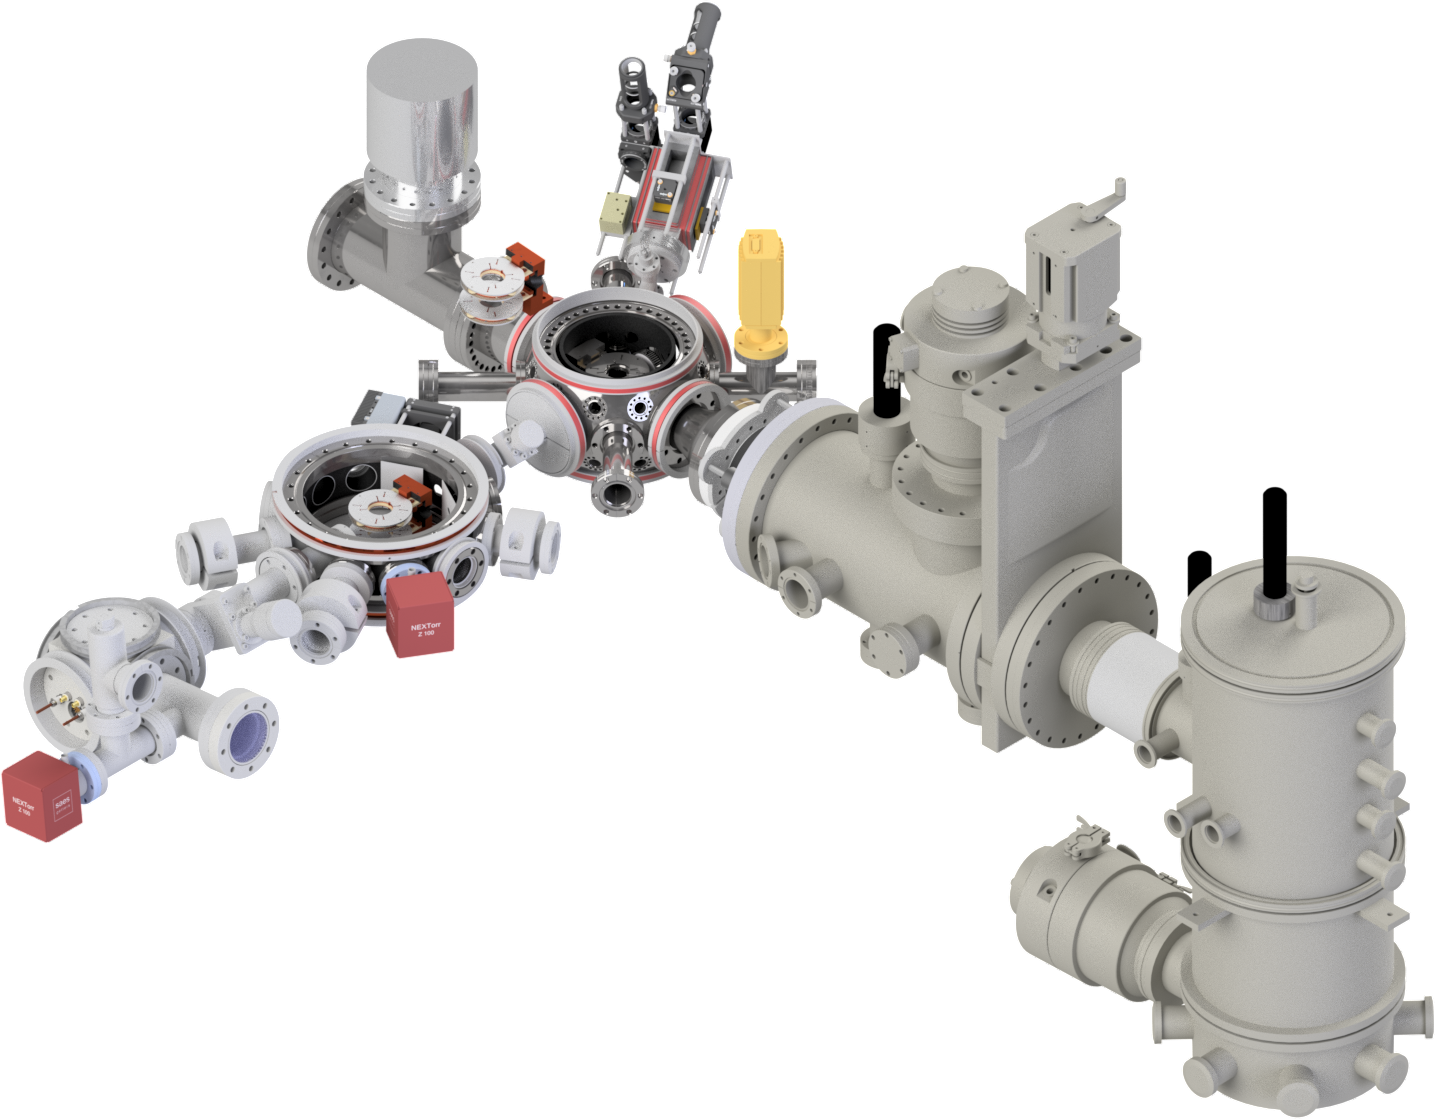
\includegraphics[width=0.8\textwidth]{figs/overview/apparatus_04_crp.png} };
      \begin{scope}[x={(image.south east)},y={(image.north west)}]
        \draw [-stealth] (0.45, 0.35) -- (0.45,0.52);
        \node[] at (0.46,0.3) {\small MOT chamber};
        \draw [-stealth] (0.18,0.23) -- (0.1, 0.3);
        \node[] at (0.21,0.2) {\small Chip chamber};
        \draw [-stealth] (0.15, 0.7) -- (0.2,0.63);
        \node[] at (0.12,0.72) {\small Tweezer chamber};
        \draw [-stealth] (0.7, 0.95) -- (0.52,0.85);
        \node[] at (0.72,0.99) {\small \Rb{} cell};
        \draw [-stealth] (0.95, 0.85) -- (0.8,0.7);
        \node[] at (0.97,0.89) {\small Slowing region};
        \draw [-stealth] (0.6, 0.2) -- (0.7,0.2);
        \node[] at (0.54,0.2) {\small Source};
      \end{scope}
    \end{tikzpicture}
  \caption[The \CaF{} experiment]{
    The \CaF{} experiment is shown along with the planned additional chip
    chamber. Not shown: external transport coils and transverse cooling region.}
  \label{overview:fig:vacuumsystem}
\end{figure}

At this point, we note that the long-lived stretched states discussed in
section~\ref{overview:existing} are promising candidates for the qubit states
in a molecule chip. For this reason it was decided that using magnetic traps,
such as those described in section~\ref{theory:chips} would be preferable to the
electrostatic traps suggested in \inlineref{Andre2006}. We are now faced with
the question of how exactly we can load molecules from the MTT into the
microscopic chip trap.

Fortunately this problem has previously been addressed for atom chips. We
discussed already in chapter~\ref{intro} that atoms can be guided on chips by
changing of trapping currents. We also discussed the transfer of
atoms between on-chip magnetic traps. For the problem of loading from a
macroscopic trap, we can turn to \inlineref{Ott2001}, where transfer from a
transport trap to a microtrap is made easier by the use of an intermediary
macroscopic trap that is well-aligned with the microtrap.
We propose a similar solution: embedding a macroscopic U-wire beneath our chip
trap which is aligned to the chip and makes a large target for loading from the
MTT.

To ensure that molecules are then loaded into the smallest trap efficiently, we
again follow in the footsteps of atom chips, and have designed  a series of
traps of decreasing size~\cite{Reichel1999}. For magnetic traps, the width of
the wires should decrease, so that the molecules remain localised around the
trap centre throughout loading. 
%
Each wire trap will begin trapping at one height before the bias field is
increased to bring the trap centre closer to the surface (as per
\myeqref{theory:eqn:height}). We choose the wires to be Z-traps so as to avoid
any losses by spin-flips, and so we label the stages $\mathrm{ZX_i}$ for
initial (higher) traps and $\mathrm{ZX_f}$ for the final (lower) trap, with
$\mathrm{ZX}$ corresponding to the wire labels in
\mytableref{overview:table:wires}. Bias fields for all traps are to be provided
by external Helmholtz coils.

Each Z-wire should be sufficiently large to maintain the currents required to
form a trap at height $z$ below the trap, whilst having a width and height  $w,
h \ll z$ so that that the current is highly localised compared to the cloud
size.
%
In the case of the first Z-wire, the molecules are still \SI{3}{\milli\meter}
away from the trapping wire. If we demand a trap depth of
$k_B\times\SI{1}{\milli\kelvin}$, then we require a trapping current of
\SI{30}{\ampere} to form a trap of this depth.  We will discuss in
chapter~\ref{fab} that the maximum wire height that can reliably be fabricated
is \SI{5}{\micro\meter}, and we expect that the wires will be able to carry a
maximum current density of \SI{6E10}{\ampere\per\meter\squared}, as was found
for a similar chip design in \inlineref{Treutlein2008}. Consequently, the
required width of the first Z-wire is $w=\SI{200}{\micro\meter}$. The currents
and widths of other wires are calculated similarly.
%
All wires have been designed to
carry twice the current that is required in the loading scheme, so that there
is sufficient headroom for further experiments, and to reduce risk of
accidental damage to the chip during normal operation.
%
The axial length of the wires also decreases to gradually reduce the size of
the trapped cloud in the $x$ direction.  

\begin{table}
  \centering
\begin{tabular}{lrrrrr}
  \hline\hline
  Name & Axis length (\si{\milli\meter}) & Width (\si{\micro\meter})& $I_\text{max}$ & Trap height (\si{\micro\meter}) \\
 \hline
  U & 16 & N/A& 100 & 3000\\
  $\mathrm{Z0}$ & 12 & 200& 60& $3000\rightarrow1000$ \\
  $\mathrm{Z1}$ &  6 & 20& 6& $1000\rightarrow100$ \\
  $\mathrm{Z2}$ &  2 & 9& 2.7& $100\rightarrow10$ \\
 \hline
\end{tabular}
  \caption[Trapping wire properties]{
    Details on the wire dimensions, maximum current, and desired
  trapping heights. The wire design is shown in
  \myfigref{overview:fig:chiplayout}. Note that the U-wire current is
  limited by vacuum feedthroughs and not by the maximum current calculated by
  the wire dimensions.  The maximum currents have been designed for use at only
  50\% of their potential maximum ($I_\text{max}$).
  }
  \label{overview:table:wires}
\end{table}

The final chip design was informed both by the requirements here, the
simulations presented in chapter~\ref{sim} and the restrictions due to the
fabrication process, which will be discussed in chapter~\ref{fab}. We tried
various different designs, but the final one that was chosen is shown in
\myfigref{overview:fig:chiplayout}. It features the wires as stipulated in
\mytableref{overview:table:wires}, fanouts for connection of macroscopic
current delivery wires, and various other features that will also be explained
in chapter~\ref{fab}.

\begin{figure}[ht]
  \centering
    \begin{overpic}[abs, width=0.51\textwidth]{figs/chip_present4.pdf}
      \put(10, 160){\small (i)}
      \put(60, 160){\small(ii)}
      \put(175, 60){\small(iv)}
      \put(110, 137){\small(iii)}
      \put(70, 90){\small \SI{20}{\micro\meter}}
      \put(112, 93){\small\SI{10}{\micro\meter}}
      \put(8, 42){\small $\mathrm{Z_0}$}
      \put(8, 10){\small $\mathrm{Z_1}$}
      \put(8, 200){\small $\mathrm{Z_2}$}
    \end{overpic}
  \caption[Chip schematic]{
    A schematic of the single-layer chip features, with the scaling exaggerated
    for visibility. The three overlapping Z-wires are shown and labeled. The
    gaps between the wires are highlighted.
    %
    Toward the left (i) is the
    electroplating connection pad and various features used for
    characterisation (ii). On Z2 it is possible to see several small pads used
    as anchors, to secure the thin wire to the substrate.  The axis of the
    $\mathrm{Z1}$ wire is labeled for reference (iii) and the other wires are
    similar. All of the above features  will be discussed further in
    chapter~\ref{fab}. The crest of Imperial College London (iv) is also
    included.}
  \label{overview:fig:chiplayout}
\end{figure}

Notice that this design is a single-layer design, with the wires intersecting.
A system has been devised to ensure that the desired currents are achieved in
each wire segment, and is described in chapter~\cm{somehwere}. Furhter, this
inital design does not incorporate microwave guides. These are to be
installed on a second level, separated from the trapping wires by a thin
insulating layer, on which we can fabricate coplanar waveguides~\cite{1127105}.
This stage of the project has not yet been reached, but the planned fabrication
procedure for microwave guides is discussed in section~\ref{fab:planned} and
their operation is discussed in chapters~\ref{mws} and \ref{squeeze}.

\begin{figure}[htb]
    \centering
    \begin{tabular}[t]{c}
\begin{subfigure}{\textwidth}
    \centering
    \smallskip
    \begin{overpic}[abs,
      width=\textwidth]{figs/exper/labeled_explosion.pdf}
      \put(20, 132){(a)}
    \end{overpic}
\end{subfigure}
    \\[1cm]
        \begin{tabular}{cc}% if you add [t], than sub images are pushed down
        \smallskip
            \begin{subfigure}[t]{0.45\textwidth}
                \centering
                \begin{overpic}[abs, width=\textwidth]{figs/overview/chamber_xsecarrow.pdf}
                  \put(5, 160){(b)}
                \end{overpic}
              \end{subfigure}&
            \begin{subfigure}[t]{0.45\textwidth}
                \centering
                \begin{overpic}[abs, width=\textwidth]{figs/chip_pic_crop.png}
                  \put(1, 160){(c)}
                \end{overpic}
            \end{subfigure}
        \end{tabular}
    \end{tabular}
  \caption[Chip experiment details]{
  The chip experiment is shown in detail. In (a) we show an exploded view of
  the chip flange assembly, with the various components labeled.
  A cross section of the chip chamber is shown in (b). The arrow shows how
  molecules will enter the chamber, brought in by the MTT.
  In (c) we have the chip assembly fully constructed, with a view of the
    aluminium-core PCB (subchip) for current delivery. The
    microwave feedthroughs remain disconnected.
  }
  \label{overview:fig:chipchamber}
\end{figure}

To facilitate all of this, the chip is mounted on a flange with supporting
infrastructure, as detailed in \myfigref{overview:fig:chipchamber}. This chip
flange assembly is equipped with a large copper heat sink, a large U-wire to
form the macroscopic alignment trap and a subchip for current and microwave
delivery. It is mounted into a recess in the subchip so that it is flush with
the surface. The chip is mounted facing downwards so that molecules can be
dropped for imaging as they fall. The flange itself is fitted with two
high-current (\SI{100}{\ampere}) feedthroughs, a 16-pin feedthrough rated for
\SI{3}{\ampere} currents, and microwave feedthroughs. All access to the chip is
therefore through this one flange, allowing for easy access and assembly.  It
will be housed in a separate vacuum chamber (the chip chamber), positioned as
shown in \myfigref{overview:fig:vacuumsystem}. The chip chamber will be
arranged so that molecules can be brought in along the transport axis (shown by
the arrow in the \mysubfigref{overview:fig:chipchamber}{b}) and positioned
below the surface of the chip.  This arrangement will be explained in further
detail in chapter~\ref{exper}.


\chapter{Simulating the trap}
\label{sim}
In this chapter I present simulations of the molecules in the trap. In
particular I show that we have developed a procedure for loading molecules into
the chip trap.

\section{Motion of molecules in a trap}
\label{sim:motion}

We can assume that the motion of the molecules in the trap is classical. They
move in the potential $V(t, \mathbf{q}) = \mu B(t, \mathbf{q})$, where
$\mu\approx\mu_B$ is the magnetic dipole moment of the molecule in the
$\ket{N=0,F=1,m_F=1}$ state.  The motion of any one particle is described by Hamilton's
equations,~\cite{Lichtenberg1969}
%
\begin{align}
  \label{sim:eq:hamilton}
  \dot{\mathbf{q}} =  \frac{\partial H}{\partial \mathbf{p}} &&
  \dot{\mathbf{p}} = -\frac{\partial H}{\partial \mathbf{q}},
\end{align}
%
where $H$ is the classical Hamiltonian of the system
\begin{equation}
  %
  H(t, \mathbf{q}, \mathbf{p}) = \frac{\mathbf{p}^2}{2m} + V(t, \mathbf{q}).
\end{equation}
For now we neglect the time dependence of the potential, so that $V(t,
\mathbf{q}) = V(\mathbf{q})$.

Solving Hamilton's equations tells us the position and momentum of a single
particle. Taken together these two vectors describe a point in a six
dimensional phase-space of position and momentum.
%
For an ensemble of particles we often consider the envelope of the region they
occupy, calling this space the phase-space volume of the ensemble. This is a
powerful tool, since calculating the trajectory of particles on the boundary of
this region is often sufficient to describe the behaviour of the whole
ensemble. This technique is commonly used in particle trapping, and especially
when considering the behaviour of beams of particles, where a four-dimensional
phase-space is used \cite{Hand1998, Lichtenberg1969}.

It is helpful for us to write the phase-space volume $V$ in terms of the
spatial volume occupied by the ensemble ($V_\text{space}$) and its temperature.
This is possible because in thermal equilibrium the momentum distribution is 
%
\begin{equation}
  f(p) = \frac{1}{(2 \pi m k_B T)^\frac{3}{2}}\exp(-\frac{p^2}{2 m k_B T})
\end{equation}
%
whose maximum value
%
\begin{equation}
  \left(\frac{\lambda_\text{dB}(T)}{h}\right)^3 = \frac{1}{(2 \pi m k_B
  T)^\frac{3}{2}}
\end{equation}
%
depends only on the temperature $T$. Here we have introduced the de Broglie
wavelength $\lambda_\text{dB}(T)$, the length-scale for a monatomic gas of
temperature $T$.~\cite{blundell2}

The unitless phase-space volume is
%
\begin{equation}
  V = V_\text{space} \lambda_\text{dB}^{-3}(T).
\end{equation}
%
It is also useful to define a unitless phase-space
density~\cite{PhysRevA.52.1423}
%
\begin{equation}
  \rho = \frac{N}{V} = \frac{N \lambda_\text{dB}(T)^3}{V_\text{space}}.
\end{equation}
%
For a given cloud with uniform phase-space density $\rho$, trap with volume
$V_\text{trap}$ and depth $T_\text{depth}$, the maximum possible number of
particles that can be trapped is $\rho V_\text{trap}/\lambda_\text{dB,
trap}^3$, where $\lambda_\text{dB, trap} = \lambda_\text{dB}(T_\text{depth})$.

A second powerful tool for determining the motion of the particles is
Liouville's theorem~\cite{Landau1982, Hand1998} which states that the phase-space
volume is a conserved quantity, as long as the trapping potential is
conservative. This means that the phase-space density of a trapped molecular
cloud cannot be increased without application of some velocity-dependent
force, such as an optical molasses~\cite{Metcalf1999}. The impact of this for
the chip is that the phase-space density of the cloud at the point of loading
onto the chip determines the maximum number of molecules that can be trapped in
the final trap.

% This calculation in Mathematica notebook 2022-01-20
If we do not introduce any further cooling steps, then the number of molecules
we are able to contain in the final trap will be
%
\begin{equation}
  N_\text{final} = \frac{\rho_\text{\CaF{}}V_\text{trap}}
  {\lambda_\text{dB, trap}^3} = \frac{\rho_\text{\CaF{}} V_\text{trap}(2 \pi m k_B
  T_\text{trap})^\frac{3}{2}}{h^3}.
  \label{sim:eq:psd_N}
\end{equation}
%
Phase space densities of $\rho_\text{\CaF{}} \sim 10^{-8}$ can be achieved by
laser cooling\footnote{Even higher phase-space densities (of the order
  $10^{-4}$) have been achieved using a cross-dipole trap~\cite{Anderegg2019a},
  but for now this is beyond the capabilities of our
experiment}~\cite{PhysRevLett.121.083201}. The smallest trap will have volume
$V_\text{trap}\sim(\SI{10}{\micro\meter})^2\times\SI{1}{\milli\meter}$ and
depth $T_\text{trap}=\SI{4}{\milli\kelvin}$, which can be calculated by
equation~\ref{theory:eqn:depth}.
%
We therefore expect that as many as $10^5$ molecules can be trapped.

In the current experiment we are not able to implement a dipole trap, although
this technique is being developed within our group. Using sub-Doppler cooling
techniques, the maximum phase
space density that we can achieve is much lower, at $\rho_\text{\CaF{}} =
3\times10^{-12}$ meaning the number of molecules trapped will be of order one.
Clearly we require the high phase-space density cloud to efficiently load the
final trap, however it will still be possible to load molecules into the outer
traps with the techniques available to us. By carefully designing a loading
scheme, we hope to be able to maximise the number of molecules that will be
accepted in the final trap.


\subsection{Phase-space acceptance}

For a particle to be trapped it must occupy some spatial region that is within
the trapping potential and it must not have sufficient energy to escape from
said potential. In other words, the total energy of the particle, given by the
classical Hamiltonian $H(\mathbf{q}, \mathbf{p})$, must be less than the trap
depth $k_B T_\text{depth}$.  This relation defines a region of phase-space that
we call the acceptance. Any particles within this region will not have
sufficient energy to escape, and so will remain trapped under classical motion
unless externally influenced (ignoring for example any collisions, decays,
Majorana losses, etc.)~\cite{Lichtenberg1969}.

As an example consider the one-dimensional case of a harmonic trap found in 
\inlineref{Crompvoets2005}
%
\begin{equation}
  V(z) = \begin{cases}
    0 & |z| > l \\
    \frac{1}{2}m\omega^2 z^2 & |z| \leq l.
  \end{cases}
\end{equation}
%
Here, any particle which starts with a position $-l \leq z \leq l$ will be
trapped, so long as its velocity is not sufficiently large that it will escape
into the $|z|> l$ region. To reach $z=l$ from an initial position $z_0$, the
particle must have kinetic energy of at least
%
\begin{equation}
  \frac{1}{2}mv_0^2 = \frac{1}{2}m\omega^2(l^2 - z_0^2),
\end{equation}
%
where $v_0$ is the initial velocity. It is now clear that a particle is trapped
on the condition that
%
\begin{equation}
  (v_0/\omega)^2 + z_0^2 < l^2
\end{equation}
%
which defines an ellipse in phase-space.

% Note that in the simulation I have omega = 1, so taking omega -> 1000 means
% that we end up with the nice circle with v in m/s. The consequence is that
% the simulation ends up lasting 1.2ms rather than 1.2s

This trapping condition can be verified by simulation, as is shown in
\myfigref{sim:fig:psaeg} (a) and (d), where the trap has been simulated for
$m = 1$, $\omega = \SI[parse-numbers=false]{10^3}{\radian\per\second}$ and $l
=\SI{1}{\milli\meter}$. We initialise 2000 particles uniformly distributed with
$|z_0| < \SI{0.2}{\milli\meter}$ and $|v_0|< \SI{1.5}{\meter\per\second}$.
Their trajectories are computed for \SI{1.2}{\milli\second} by the methods
described in the next section. The boundary of the acceptance, called the
separatrix is shown in black. All particles that are initialised inside the
acceptance remain trapped and evolve through time in the usual way for a
harmonic potential.  Particles initialised outside the acceptance are rejected
and lost.

It is also instructive to consider anharmonic potentials, for example
%
\begin{equation}
  V(z) = -V_0\cos(\omega z)
\end{equation}
%
which is also presented in \myfigref{sim:fig:psaeg}, using the same
parameters as for the previous potential. We again see that particles with
sufficiently low energy in the trapping region remain trapped, however in this
case the anharmonicity of the trap results in the particle cloud spiralling
outwards, undergoing an effective increase in the phase-space density. This
means that although the actual phase-space density remains the same, the
envelope of the region that they occupy becomes increasingly convoluted. This
makes it effectively impossible to contain them in any potential with a volume
smaller than that of the trapping potential. This effect is often referred to
as filamentation.

Finally, it is useful to consider the phase-space acceptance of a wire trap.
For simplicity we begin by considering only the acceptance in the $z$ direction
(perpendicular to the chip surface). We calculate the acceptance of a Z-wire
with an axis of \SI{20}{\milli\meter}, current of \SI{40}{\ampere} and a
trapping height of \SI{3}{\milli\meter}. The particles are initialised such
that they have no motion in the $x$ and $y$ directions, and the trajectories
are simulated for \SI{200}{\milli\second}. Figures~\ref{sim:fig:psaeg}~(c)
and (f) show the distribution at the start and end of the simulation.
The accepted molecules (blue) are once again those that start inside the
separatrix. There are also metastable molecules (orange) which remain outside
the acceptance but stay nearby the trap. These are molecules with nearly
sufficient energy to escape the trap, but may take some time to do so.
We call the occupied area of phase-space at the end of the trapping
period the trap's phase-space emittance.

\begin{figure}[htb]
  \centering
  \scalebox{0.8}{\import{figs/simsThesis/}{psa_1D.pgf}}
  \caption[Phase-space acceptance examples]{
    The phase-space acceptance for harmonic (a, d), anharmonic (b, e) and
    Z-wire trap (c, e) are shown. The top row shows the initial positions of
    the particles: those that are accepted by the trap are shaded blue,
    particles that are lost are shaded red, and metastable particles in orange.
    The energy contour of the trap depth is also shown. The end state of the
    simulation is shown in the lower row. Note the filamentation effect in (e)
    and (f), where the effective phase-space density of the particles decreases
    as they explore regions that are energetically accessible. The harmonic and
    anharmonic examples are inspired by the discussion in
    \inlineref{Crompvoets2005}.
  }
  \label{sim:fig:psaeg}
\end{figure}

While this applies to a rapid switching off and on of trapping potentials, we
note that it is possible to adiabatically transform potentials in such a way
that the phase-space density of the ensemble remains unchanged. This can be
achieved because the Liouville theorem also holds for time-dependent
Hamiltonians, as long as the potential remains conservative
throughout~\cite{Hand1998, Lichtenberg1969}. Hence a cloud of trapped particles
can be translated, for example in the transport coils, or towards the surface
of the chip as will be discussed in section~\ref{sim:adiabatic}.

\subsection{Simulating the motion}
\label{sim:motion:simmethods}

The motion of a particle can be simulated by numerically solving
\myeqref{sim:eq:hamilton}, which we do using Python~\cite{python} and the
symplectic Euler method~\cite{Hairer2015, doi:10.1119/1.2034523} provided by
the Desolver package~\cite{desolver}. Unlike other numerical methods,
symplectic integrators guarantee the conservation of energy and momentum.
We are able to simulate any arbitrary potential, such as those already
discussed in the previous section, but it is useful to consider a more
realistic potential given by the sum of the magnetic and gravitational
potentials,
%
\begin{equation}
  V(t, \mathbf{q}) = V_\text{mag} + mg(z_0-z)
\end{equation}
where $g=\SI{9.8}{\meter\per\second\squared}$ is the acceleration due to
gravity, and $z_0$ is an arbitrary point chosen to be the zero of the
gravitational potential. The actual value chosen does not matter as it
constitutes only a linear offset in the entire potential. We choose
$z_0$ to be the minimum of the trapping potential at the start of each
simulation.
%
The Van der Waals attraction between the chip and the molecules is neglected,
since the molecules will (by design) never be close enough to the chip for this
force to be significant.

The magnetic potentials of the wire traps are calculated by considering the
traps to be formed of segments of straight wires, each producing a magnetic
field $\mathbf{B}_\text{seg}^{(i)}$, and the bias field
$\mathbf{B}_\text{bias}(t)$.  The total field is the sum of contributions from
the set of all segments ($S$), and the bias. We also make the approximation
that the field changes slowly compared to the alignment of the spin with the
field\footnote{This means that simulations investigating fast-changing fields
  present an optimistic result. However we will see below that the limiting
  factor for changing the field is the time constant of the classical motion of
  the molecules. Hence this adiabtic approximation is sufficent for our
investigations.}, so that $V=\mathbf{\mu}\cdot\mathbf{B}\approx\mu B$.  The
potential is therefore
%
\begin{equation} V_\text{mag}(t, \mathbf{q}) = \mu B (t, \mathbf{q}) = \mu
\left| \sum_{i\in S} \mathbf{B}_\text{seg}^{(i)}(t, \mathbf{q}) +
\mathbf{B}_\text{bias}(t)\right|,  \end{equation}
%
where the field of each wire segment is~\cite{Griffiths2017}
%
\begin{equation}
    \mathbf{B}_\text{seg}(t, \mathbf{q}) = \frac{\mu_0 I(t)}{4\pi
    s_\text{seg}(\mathbf{q})} (\sin(\theta_2)  -
    \sin(\theta_1))\hat{\mathbf{\phi}}.
    \label{sim:eq:segmentfield}
\end{equation}
%
Here $s_\text{seg}(\mathbf{q})$ represents the shortest distance between the
point $\mathbf{q}$ and the line that runs through the segment off to infinity
in each direction as defined in \myfigref{sim:fig:wiresegment}. We also have
the unit vector $\hat{\mathbf{\phi}} = \mathbf{I}\times\mathbf{q}/(qI)$.

\begin{figure}[h]
\centering
  \begin{tikzpicture}
    % Def coords
    \coordinate (O) at (0, 0);
    \coordinate (L) at (-3, 0);
    \coordinate (R) at (3, 0);
    \coordinate (Q) at (-4, 4);
    \coordinate (P) at (-4, 0);
    % Draw lines
    \draw[line width=0.75mm, ->] (L) -- (R);
    \draw (L) -- (Q);
    \draw (R) -- (Q);
    \draw[<->, densely dotted,shorten >=.5mm,shorten <=.8mm] (Q) -- (P);
    % Draw line parallel to wire
    \draw[-, dashed] (-5, 0) -- (L);
    \draw[-, dashed] (R) -- (5, 0);
    % Draw dot at Q
    \node at (Q)[circle,fill,inner sep=.5mm]{};
    % Draw angels
    \draw pic[->, draw,angle radius=1cm,"$\theta_1$" shift={(-3mm,-1mm)}] {angle=P--Q--L};
    \draw pic[->, draw,angle radius=1.5cm,"$\theta_2$" shift={(2mm,-2mm)}] {angle=P--Q--R};
    % Label
    \node[shift={(4mm,0)}] at (Q) {$\mathbf{q}$};
    \node[shift={(2mm, 4mm)}] at (R) {$I$};
    \node[fill=white] at (-5.0, 1.8) {$s_\text{seg}(\mathbf{q})$};
  \end{tikzpicture}
  \caption[Geometry of a wire segment]{
    Geometry of a wire segment (bold) carrying current $I$, whose field
  can be calculated using \myeqref{sim:eq:segmentfield}. The dotted line
  shows $s_\text{seg}(\mathbf{q})$, the shortest distance from the point at
  which the field is calculated ($\mathbf{q}$) to the line parallel with the
  wire (dashed line).
  }
  \label{sim:fig:wiresegment}
\end{figure}

%In the case of that we are exchanging between
%two potentials, the segments of both traps are included in the summation, with
%the currents becoming functions of time, and similar for exchange between a
%quadrupole and a wire trap, with the quadrupole gradient being a function of
%time.

\subsection{Simulation initialisation}
\label{sim:sim:init}

For all the simulations described below, we begin with a cloud of molecules in
a magnetic quadrupole trap. We use the following initialisation procedure so
that the distribution of our molecules matches that which we expect in the
experiment. 
%
The simulation begins with a cloud of $N$ molecules whose positions are normally distributed
in all three spatial dimensions with a standard deviation of $\sigma_i$
(typically $\sigma_i = \SI{1}{\milli\meter}$). Similarly the velocity components
are normally distributed with a standard deviation of $\sigma_{v_i}$ (typically
\SI{400}{\milli\meter\per\second}, corresponding to a temperature of
\SI{50}{\micro\kelvin}). 

The cloud is initialised in a quadrupole trap with gradient
\SI{10}{\gauss\per\centi\meter}. They are held for \SI{50}{\milli\second}
before the gradient is linearly ramped over \SI{100}{\milli\second} to
\SI{60}{\gauss\per\centi\meter} (the gradient used in the MTT).  The molecules are
then held for a further \SI{50}{\milli\second}, as a stabilisation time. The
increasing trap gradient compresses the distribution. The resulting
distribution is Gaussian in velocity and position, centred on
$z=\SI{3}{\milli\meter}$, as shown in \myfigref{sim:fig:initsum}.

\begin{figure}[htb]
\centering
  \import{figs/simsThesis/}{init_summary.pgf}
  \caption[Phase-space simulation initialisation]{
    The particle distribution in phase-space after initialisation. A
  scatter plot of the $z\,v_z$-phase-space plane the is shown in (a), with
  histograms of $z$ and $v_z$ distributions in (c) and (b) respectively. The
  position distributions for $x$ and $y$ are shown in (d) in orange and green
  respectively.}
  \label{sim:fig:initsum}
\end{figure}

\section{Adiabatic transfer between traps}
\label{sim:adiabatic}

It should be obvious that if we start with molecules in one potential, then
rapidly turn that one off and turn on another with a different shape, is likely
to cause heating and increase the size of the cloud.  However, if we ramp
between the traps adiabatically then we expect the phase-space density to be
conserved. In order to understand how best to load the chip trap it is
important that we understand the extent of heating in the case of rapid
transfer and the timescale required to be adiabatic.

We investigate this with a simple example: consider two ideal quadrupole traps
with gradients of \SI{60}{\gauss\per\centi\meter} separated by
\SI{3}{\milli\meter} in the $x$ direction. We simulate 2000 \CaF{} molecules
using the above-described initialisation procedure, with initial $\sigma_i =
\SI{2}{\milli\meter}$ in all directions, and initial temperature
$T=\SI{50}{\micro\kelvin}$. We ramp linearly between the potentials in a time
$t_\text{ramp}$, which we vary between \SI{1}{\milli\second} and
\SI{100}{\milli\second}. The molecules are then held for a further
\SI{100}{\milli\second}. The state of the system at the end of the simulation
is shown for $t_\text{ramp}\in \{\SI{1}{\milli\second}, \SI{30}{\milli\second},
\SI{100}{\milli\second}\}$ in \myfigref{sim:fig:adia3sim}, along with the
behaviour of the cloud in the \SI{100}{\milli\second} hold time. Note that as
the ramp time increases, the oscillation in cloud size, temperate and position
decreases, as we have said we expect.

\begin{figure}[p]
\centering
  \scalebox{0.8}{\import{figs/simsThesis/}{adiabatic_3sim.pgf}}
  \caption[Simulation of exchange between quadrupole traps]{
    Exchange between two quadrupole traps, separated by \SI{3}{\milli\meter},
    for three different ramp times. The top row shows the $x$-projection of the
    phase-space distributions of the particles at the start of the simulation
    (grey) and after various ramp times (see legend) followed by a
    \SI{100}{\milli\second} hold in the displaced trap. The mean position, size
    and temperature of the cloud are shown throughout the hold time for each
    simulation. Note that for the longer ramps we observe less severe heating,
    oscillation and widening of the cloud.
  }
  \label{sim:fig:adia3sim}
\end{figure}


The question then is at what point do we enter the adiabatic regime?
\myfigref{sim:fig:adiavary} shows the cloud width and temperature at the end
of the simulation for varying $t_\text{ramp}$. After
$t_\text{ramp}\sim\SI{50}{\milli\second}$ the reduction is minimal, and we are
strongly in the adiabatic regime. This is approximately the timescale we
would expect. Although the trap is not harmonic, we can still give the
characteristic period for a particle that has a characteristic amplitude of
motion. Assuming that the particle is under constant acceleration, the
timescale for a particle to traverse the trap is
%
\begin{equation}
  \tau = \sqrt{\frac{m \sigma}{\mu_B B'}},
\end{equation}
%
where $\sigma$ here means the width of the trapped cloud. To be in the
adiabatic regime, we expect to have any particle traverse the trap multiple
times over the duration of a ramp Our typical \CaF{}
clouds
have width $\sigma = \SI{5}{\milli\meter}$, so the timescale will be $\tau
\approx \SI{10}{\milli\second}$. We expect the adiabatic regime to
be reached when a process takes place over a duration that is several multiples
of this timescale, which is in good agreement with the simulations.

\begin{figure}[t!]
\centering
  \scalebox{0.8}{\import{figs/simsThesis/}{adiabatic_varyramps.pgf}}
  \caption[Effect of ramp duration on phase-space distribution]{
    The final temperature and size of particle clouds transferred between
    offset quadrupole traps at various ramp times. Note that the large
    oscillations in width that occur for short ramp times (see
    \myfigref{sim:fig:adia3sim}) can result in the instantaneous width of
    the cloud being small, such as in the shorter ramp times here.
  }
  \label{sim:fig:adiavary}
\end{figure}

\section{Trajectory simulation of the initial loading stages}

In this section we will present simulations of loading molecules from the MTT
into the on-chip Z-wire traps. 
This demonstrates
the two main types of transitions in the loading process: handovers between
traps, and compression within a single trap. The timing of the simulation do
not exactly reflect those that will be used in practice and long holding periods
have been inserted between ramps to better illustrate the cause of particle
loss. It is useful to perform direct trajectory simulations as opposed to
simple analysis of the phase-space emittance and acceptance, since (as we will
see later) brief lowering of trap depth during trap handovers can induce
additional loss of particles.

We will consider the handover in four stages: the particle initialisation, which
was already discussed in section~\ref{sim:sim:init}; followed by the
handover from the MTT to the U-wire; then the U-wire to $\mathrm{Z0_i}$.
Finally we will simulate the compression in the Z-wire trap from
$\mathrm{Z0_i}$ to $\mathrm{Z0_f}$. A full summary of the changing parameters
throughout the simulations is given at the end of the section, see especially
\myfigref{sim:fig:simsum}.

\subsection{MTT - U transfer}
\label{sim:sim:trans_U}

% This is PSD 3.8E-10, which is a lot lower than can reasonably be achieved.
% Might be asked to comment on this
The cloud is initialised by the usual procedure, with $\sigma_i =
\SI{1}{\milli\meter}$ and $T=\SI{50}{\micro\kelvin}$, corresponding to the
typical cloud sizes and temperatures we measure in the tweezer chamber after
transport. Over \SI{100}{\milli\second} the coil current is linearly
reduced to zero and the U-wire current is ramped up to its maximum value of
\SI{100}{\ampere}. The bias fields in the $y$ and $z$ directions (no $x$ bias
is applied) are also ramped linearly, to maintain the trap centre at a height
of \SI{3}{\milli\meter} below the chip. The state of the system before and
after the ramp is shown in \myfigref{sim:fig:mttusim}.

\begin{figure}[p]
\centering
  \scalebox{0.8}{\import{figs/simsThesis/}{mtt_u_summary.pgf}}
  \caption[Simulation of transfer from MTT to U-trap]{
    The simulation of the transfer from the MTT to the U-wire. The state of the
    system is presented at the end of the initialisation procedure (blue) when
    the trapping potential is that of the MTT, and after ramping to the U-trap
    (red). The phase-space distributions are shown in the $z$-$v_z$ plane in
    (a) and (b), with histograms of the $z$ and $v_z$ projections in (c) and
    (e) respectively. The potentials at the start and end of the transfer are
    shown in (d). Subfigure (f) shows the temperature and the particle number
    varying throughout. Transfer occurs during the times that are shaded grey
    (c.f.~\myfigref{sim:fig:simsum}).
  }
  \label{sim:fig:mttusim}
\end{figure}

The phase-space distribution in the $z$-$v_z$ projection is shown for the start
(\mysubfigref{sim:fig:mttusim}{a}) and end
(\mysubfigref{sim:fig:mttusim}{b}) of the simulation. Note that there is
little change to the velocity distribution, but in position the particles shift
to occupy the positive $z$ direction, where the potential is less steep.

Looking at the change in the particle number throughout the ramp (grey region
of \mysubfigref{sim:fig:mttusim}{f}) it is clear that there is some particle
loss. We would naively expect there to be no loss during this transfer, since
the final trap depth is larger than the temperature of the cloud, and there is
good mode-matching of the two potentials. To see why this loss occurs, we  look
at the evolution in phase-space for each projection throughout the ramp, as
shown in \myfigref{sim:fig:mttudetail}.

\begin{figure}[htp]
\centering
  \begin{tabular}{c}
    \scalebox{0.8}{\import{figs/simsThesis/}{mtt_u_detail_x.pgf}} \\
    \scalebox{0.8}{\import{figs/simsThesis/}{mtt_u_detail_y.pgf}} \\
    \scalebox{0.8}{\import{figs/simsThesis/}{mtt_u_detail_z.pgf}}
  \end{tabular}
  \caption[Phase-space distribution throughout MTT-U handover]{
    Each pair of rows shows the phase-space plots for the MTT to U-trap
    handover simulation in the $q_i$-$v_i$ plane, along with the cut-through of
    the potential through the trap centre along $q_i$ at various times. This
    supplements the simulation summary shown in \myfigref{sim:fig:mttusim}.
    The superposition of the quadrupole and U-traps briefly causes a lowering
    of the trapping potential, as can be seen at \SI{75}{\milli\second}. These
    reductions can occur when moving between different types of traps, such as
    from the coil-based to wire trap, or from a quadrupole to Ioffe-Pritchard
    trap. Care must be taken in such cases to ensure the potential is
    sufficiently deep throughout the handover.
}
  \label{sim:fig:mttudetail}
\end{figure}

At $t=\SI{75}{\milli\second}$ there is a noticeable decrease in the trapping
depth in the $-y$ and $+z$ directions. This is the cause of the particle leak,
and occurs due to the due to the superposition of the two fields causing an
overall decrease in the trap depth. When the trap depth is increased again, the
energy of particles in this region is increased, and they can leave the trap.
This only occurs for a brief period during the ramp (lasting approximately
\SI{40}{\milli\second}).  Hence some of the more energetic particles are lost,
as can be seen in the figure. The key finding is that the molecules are able to
be transferred from the MTT to the U-trap with minimal loss by mode-matching of
the potentials.

\subsection{U - Z transfer}
\label{sim:sim:U_to_Z0i}

The next stage of loading is the U to $\mathrm{Z0_i}$ handover. We simulate
this process as a continuation of the MTT-U transfer.  The Z-wire current is
then linearly ramped on over \SI{100}{\milli\second} to \SI{30}{\ampere}, while
the U-wire current is ramped off. The
bias fields are linearly ramped to maintain the trap height at
\SI{3}{\milli\meter}. The simulation is presented in \myfigref{sim:fig:uzsim},
and the ramps are summarised in \myfigref{sim:fig:simsum}.

In the former figure we have the initial (a, blue) and final (b, red) particle
distributions.  With the $z$ velocities and positions summarised in the
histograms in (c) and (e) respectively. We can see that the mean position and
velocity remains the same, but it is clear from (b) that there are a number of
particles that have picked up velocity in the positive $z$ direction, and can
be seen leaving the trap. This is the notable streak to the right of the
subfigure, and can also be seen in the tail of the histogram in (e). The
particle number decreases by 20\% as seen in (f), although the particles do not
fully leave the trap until the next step (see \mysubfigref{sim:fig:simsum}{d}).
This loss is similar to that of the MTT to U-trap handover, with a decrease in
trap depth that we attribute from changing from a quadrupole to Ioffe-Pritchard
trap. This changeover can be seen in (d) where we note that the final trapping
potential's minimum is non-zero. Despite the particle losses there is minimal
change to the particle distribution

\begin{figure}[p]
\centering
  \scalebox{0.8}{\import{figs/simsThesis/}{u_z_summary.pgf}}
  \caption[Simulation of transfer from U-trap to Z-trap]{
    The simulation of the transfer from the U-wire to the Z-wire. The state of
    the system is presented at the end of the initialisation procedure (blue)
    when the trapping potential is that of the U-trap, and after ramping to the
    Z-trap (red). The phase-space distributions are shown in the $z$-$v_z$
    plane in (a) and (b), with histograms of the $z$ and $v_z$ projections in
    (c) and (e) respectively. The potentials at the start and end of the
    transfer are shown in (d). Subfigure (f) shows the temperature and the
    particle number varying throughout the simulation. Transfer occurs during
    the times that are shaded grey (c.f.~\myfigref{sim:fig:simsum}).

  }
  \label{sim:fig:uzsim}
\end{figure}

\subsection{Z compression}

The final stage of the loading procedure is a linear ramp of the trap height
from \SI{3}{\milli\meter} below the chip surface to \SI{1}{\milli\meter} below.
Here only the $y$ bias field is changed so  that the trap depth
increases and the cloud is compressed, providing good localisation of the
molecules. Ramping the height linearly requires the bias to change as a
function of time so that $\tilde{B}_{y} \propto t^{-1}$.

As can be seen in \myfigref{sim:fig:zsim}, there is particle loss,
although much of this is due to particles that had already left the trapping
region in the previous ramp. As can be seen in subfigure~(f), the particle
number is decreasing before the ramp begins. The other major effect of the ramp
is heating, which occurs due to the spatial compression and conservation of
phase-space density.
%
The transfer of the cloud towards the chip surface is successful, as can be seen
in \mysubfigref{sim:fig:zsim}{e}, the particles are highly localised around the
new trap minimum at $z=\SI{1}{\milli\meter}$.

\begin{figure}[p]
\centering
  \scalebox{0.8}{\import{figs/simsThesis/}{z_summary.pgf}}
  \caption[Simulation of compression in Z-trap]{
    The simulation of the compression in the Z-wire trap. The state of the
    system is presented at the end of the initialisation procedure (blue) when
    the trapping potential minimum is held \SI{3}{\milli\meter} from the
    surface, and after compressing to the height of \SI{1}{\milli\meter} (red).
    The phase-space distributions are shown in the $z$-$v_z$ plane in (a) and
    (b), with histograms of the $z$ and $v_z$ projections in (c) and (e)
    respectively. The potentials at the start and end of the transfer are shown
    in (d). Subfigure (f) shows the temperature and the particle number varying
    throughout the simulation. Transfer occurs during the times that are shaded
    grey (c.f.~\myfigref{sim:fig:simsum}).
  }
  \label{sim:fig:zsim}
\end{figure}

\subsection{Summary of the simulation}

The entire simulation from MTT to $\mathrm{Z0_f}$ is summarised in
\myfigref{sim:fig:simsum}. For each stage: initialisation (a), MTT-U
transfer (b), U-Z transfer (c) and Z compression (d) the particle number is
shown. The total temperature and cloud width are also given for the particles
that remain in the trap at the end of the simulation. The profile of parameters
that are changed for each ramp are also shown. 


\begin{figure}[p]
\centering
  \scalebox{0.8}{\import{figs/simsThesis/}{total_summary.pgf}}
  \caption[Summary of loading simulations]{
    Details for each stage of the simulation in turn. The top two rows show
    properties of the molecule cloud and the second two rows show the trapping
    currents and bias fields throughout. Column (a) shows the initialisation
    procedure. Column (b) shows the ramp from the MTT to U-wire, with the ramp
    duration shaded grey.  In column (c) we have the U-Z handover and the $z$
    bias field is switched off. Finally in column (d) is the compression in the
    Z-trap.
  }
  \label{sim:fig:simsum}
\end{figure}

The simulation shows that the loading of the initial chip trap can bring in
approximately 60\% of the initial cloud. We assumed an initial temperature of
\SI{50}{\micro\kelvin}, however refining the transport process could allow us
to load clouds of lower temperatures, which could mean that a higher loading
efficiency is possible. It may also be possible to implement cooling during the
trap transfer, but this is restricted by the limited optical access in the chip
chamber.
%
There is some expansion of the cloud as molecules are lost, particularly caused
during the U-Z handover stage.
%
Heating in the trap is largely due to the compression in the final stage. This
is inevitable, but does not cause any problems, since the trap depth
increases for traps closer to the surface, and the molecules are
well contained.

The trajectory simulation discussed in this section is instructive, since it
tells us about the handovers between different types of traps. Notice
that the largest source of particle loss is when converting from the quadrupole
U-trap to the Ioffe-Pritchard Z-trap. Here it is not sufficient to look just at
the phase-space emittance and acceptance in the final traps, but we must
investigate the potential across the ramp, since a brief lowering of the
potential can induce enormous loss. Fortunately this is not an issue when
compressing and handing over between Z-traps, and the phase-space analysis is
sufficient for the rest of the procedure.

\section{Phase-space acceptance of remaining Z-traps}
\label{sim:transferbetweenzs}

Once trapped in $\mathrm{Z0_f}$, the remaining loading stages are simply
repeated handovers to the smaller wires, with a compression stage carried out
on each wire to bring the molecules closer to the surface. This is a
well-understood and robust procedure that has been used before to load atom
chips with minimal losses~\cite{Reichel2002}. The ramps used are detailed in
table~\ref{overview:table:wires}.  The timing of the ramps could be shorter for
the Z-traps, since the timescale of motion in these traps is higher. This, as
well as the optimal shape of the ramp can be determined empirically.

That said, since our experiment will operate with a significantly lower phase
space density than previous experiments with atoms, it is important to ensure
that our loading procedure will not suffer from any unnecessary losses. These
compressed traps contain hotter molecules, requiring a smaller time step for
simulation. It is therefore easier to directly examine the acceptance of each
trap. We also note now that the trap gradients are sufficiently large the
effects of gravity can be ignored.

The trap acceptances are shown in \myfigref{sim:fig:phasematchinggrid},
starting with $\mathrm{Z0_f}$ in row (a). The region of the trap that we expect
to be occupied (as determined by the simulation above) is marked with a dashed
line.  This cloud of molecules will be adiabatically transferred into
$\mathrm{Z1_i}$.
%
The cloud of molecules will be transferred to $\mathrm{Z1_i}$ with negligible
heating. However, the total acceptance of the trap is less than the expected
phase-space volume of the cloud. We can estimate the spillover loss t be 73\%
on the phase-space volumes in
\myfigref{sim:fig:phasematchinggrid}. Performing the handover adiabatically
will maximise the number of molecules that can be transferred.

Next, $\mathrm{Z1_i}$ is adiabatically compressed to $\mathrm{Z1_f}$, with the
molecules held \SI{100}{\micro\meter} from the surface, as shown in row (b).
The particles will undergo filamentation, exploring all regions that are
energetically accessible and increasing the effective phase-space volume that
they occupy. This expected occupation region is calculated from the
energy-contour in phase-space that matches the temperature of the cloud, and is
marked by the dotted line. There is now handover into $\mathrm{Z2_i}$, with the
particles inside the phase-space acceptance contained in the new trap. We
expect spillover losses of 84\%. In the final stage the trap is compressed,
into $\mathrm{Z2_f}$, during which we expect no loss. The final occupation is
shown in \mysubfigref{sim:fig:phasematchinggrid}{c}.
%
Particle loss during the procedure can be estimated from the mismatching of
these phase-space emittances and acceptances.

\begin{figure}[tbhp]
\centering
  \scalebox{0.8}{\begin{overpic}[page=1]{figs/simsThesis/phase_matching_grid.pdf}
    \put(0,68){(a)}
    \put(0,44.5){(b)}
    \put(0,21){(c)}
  \end{overpic}}
  \caption[Mode-matching on-chip traps]{
    The acceptance (solid) and expected occupation (dashed) of each Z-wire
    trap. This is calculated by finding the acceptance in the weak ($x$)
    trapping direction. Row (a) shows $\mathrm{Z0_f}$, with occupation
    determined by the above simulation. Molecules will be adiabatically
    transferred to $\mathrm{Z1_i}$, which will be fully occupied. Some
    particles will be lost due to the decrease in acceptance but this is to be
    expected, and phase-space density should not increase. In (b) we have the
    acceptance and occupation of $\mathrm{Z1_f}$ following adiabatic
    compression.  Particles will be adiabatically transferred into
    $\mathrm{Z2_i}$, resulting in similar losses to the previous step. Row (c)
    shows the final acceptance and occupation of $\mathrm{Z2_f}$.
  }
  \label{sim:fig:phasematchinggrid}
\end{figure}


The above-described spillover losses can be combined with the loading
efficiency determined by the trajectory simulations. We expect a total loading
efficiency of 2\%. This would deliver only 50 molecules into the final trap in
what is a highly-idealised loading simulation. Notably the analysis of the
phase-space acceptance does not account for decrease in effective phase-space
density by filamenation, which will further reduce the final occupation. This
confirms that we will need to produce a much higher initial phase-space density
to load a sufficiently large number of molecules into the trap. However it is
clear that this procedure can be applied to much higher density clouds, such as
those which can be produced using optical dipole traps. Ongoing efforts to
produce higher density clouds of \CaF{} could improve this final molecule
number even further.

\section{Summary}

In this chapter I have presented the design of the chip experiment, starting
with the source of molecules up to the stage of confinement in a Z-trap
\SI{10}{\micro\meter} from the chip surface. I have presented
a loading procedure that will allow us to load this final trap through a series
of wire traps of decreasing size. This is justified by simulation and
phase-space analysis of the acceptance of the various trapping stages.
%
The design leaves scope for the addition of microwave guides on a second layer
above the trapping wires, as discussed in section~\ref{theory:chips}.


\chapter{Microfabrication}
\label{fab}
Fabrication of a chip has been an iterative process, where we have
simultaneously improved upon both the chip's design and our fabrication
techniques.
In this chapter I will present the progress that we have made in
learning how to build a chip trap, and how we plan to integrate a microwave
guide in future experiments. 

All the microfabrication techniques described below except for the
electroplating were undertaken at the London Centre for Nanotechnology (LCN). 

\section{Overview of the fabrication procedure}

% TODO I grabbed this Madou2002 citation from Treutlein, but I should ensure
% that it is legit
Our trap has been designed so that the size of the wires is small compared to
the size and height of the trapped cloud. As such trapping wires on the chip
are as small as \SI{3}{\micro\meter} in width. Such small features can be
produced using standard photolithography techniques~\cite{Madou2002}. However,
the maximum height of features produced in these procedures is usually of the
order \SI{100}{\nano\meter}.

% TODO Need to cite this $j$ number and probably revise this based on what we
% actually say in design chapter. I don't think I need this caluclation here
We must ensure that the wires are capable of carrying the currents that are
outlined in chapter~\ref{design}.  Other experiments with two-layer atom chips
have reported a current density of $j=\SI{6E10}{\ampere\per\meter\squared}$ in
the trapping wires. For our wires this would require a minimum height of $h
\sim I w/j = \SI{1}{\ampere} \times
\SI{10}{\micro\meter}/\SI{6E10}{\ampere\per\meter\squared} \sim
\SI{1}{\micro\meter}$  to carry our trapping currents.This is much higher than
can be achieved with photolithography techniques.

To achieve the required height, we have used through-mask
electroplating~\cite{Ruythooren_2000}. First a substate is coated with a thin
seed layer of gold, then photolithography is used to produce a thick (several
mircron high) mould. The mould covers regions where no further deposition is
required. The substrate can then be electroplated, with the seed layer acting
as the anode, allowing thick wires to be deposited into the mould.
After electroplating the seed layer can be etched away. This is a common
technique for constructing atom chips and is described in \inlinerefs{2011Ac,
Lev2003, KOUKHARENKO2004600}.

The fabrication process for our final chip begins with a four inch silicon
wafer, which we dice into individual \SI{20}{\milli\meter} by
\SI{20}{\milli\meter} dies. The remaining process can be briefly summarised:
\cm{Is there a better way to link this list to the following sections?}
\begin{enumerate}
\item Lay down thin (\SI{60}{\nano\meter}) seed layer of chromium and gold.
\item Spin coat a thick (\SI{6}{\micro\meter}) layer of photoresist.
\item Expose and develop the thick photoresist so as to create a ``mould''
in the desired shape of the wires.
\item Electroplate the chip, such that wires are formed in the mould to the
desired height.
\item Remove the photoresist mould.
\item Chemically etch the chip so as to remove the seed layer and
  electrically isolate the wires.
\end{enumerate}
This process is illustrated in \myfigref{fab:fig:process}

\begin{figure}[h]
\vspace{0.8cm}
\centering
\begin{tabular}{cccc}
  %\begin{overpic}[width=0.22\textwidth]{figs/fab/cartoon/01_barewafer.pdf}
  %  \put(0,40){(a)}
  %\end{overpic} &
  \begin{overpic}[width=0.22\textwidth]{figs/fab/cartoon/03_wafercrauwarrows.pdf}
    \put(0,40){(1)}
  \end{overpic} &
  \begin{overpic}[width=0.22\textwidth]{figs/fab/cartoon/03.5_waferpr.pdf}
    \put(0,40){(2)}
  \end{overpic} &
  \begin{overpic}[width=0.22\textwidth]{figs/fab/cartoon/04_wafermould.pdf}
    \put(0,40){(3)}
  \end{overpic} \\[2cm]
  \begin{overpic}[width=0.22\textwidth]{figs/fab/cartoon/e.pdf}
    \put(0,40){(4)}
  \end{overpic} &
  \begin{overpic}[width=0.22\textwidth]{figs/fab/cartoon/f.pdf}
    \put(0,40){(5)}
  \end{overpic} &
  %\begin{overpic}[width=0.22\textwidth]{figs/fab/cartoon/g.pdf}
  %  \put(0,40){(g)}
  %\end{overpic} &
  \begin{overpic}[width=0.22\textwidth]{figs/fab/cartoon/h.pdf}
    \put(0,40){(6)}
  \end{overpic}
\end{tabular}
  \caption{
    Illustration of the fabrication process. We begin with in (1) with a
    silicon die (black), on which we deposit chromium adhesion layer (grey) and
    a seed layer of gold (yellow). In (2) the entire die is spin coated in
    photoresist (purple). The mould is formed by photolithography techniques
    (3) and then electroplating is used to form tall wires (4). The photoresist
    is removed (5), and then a gold etch followed by a chrome etch (6) are used
    to electronically isolate the features.
  }
  \label{fab:fig:process}
\end{figure}

As discussed in chapter~\ref{intro}, a future aim of the molecule chip project is to
integrate microwave guides on the chip. These guides must allow good overlap of
the microwave fields and the molecule trapping region. Our design achieves this
by positioning the microwave guides on a second layer, directly above the
trapping wires. We have not yet attempted the following stages of
fabrication, but we anticipate that they will be:
\begin{enumerate}[resume]
    \item Spin coat chip with an insulating layer of polyimide.
    \item Perform standard photolithography to lay down microwave guides on the
      chip.
\end{enumerate}
These steps are discussed further in section~\ref{fab:planned}.

In the rest of this chapter I will describe the above process in detail,
including the various pitfalls that we found as we itterated towards a complete
\cm{trapping chip}.

\section{Metal evaporation of seed layer}

Before any fabrication, the die must be cleaned and dehydrated to ensure that
there will be good adhesion to the substrate. A solvent clean with acetone and
isopropyl alchol will remove any organic compounds \cm{check this}. The die is
then rinsed with deionised water and dehydrated in an oxygen plasma for ten
minutes.
The die is then ready for metalization, which here is done by metal
evaporation. To further improve adhesion between the gold and silicon, a thin
($<10\si{\micro\meter}$) intermediary chrome layer is deposited first, followed
by \SI{50}{\micro\meter} of gold.

We performed evaporation using an Edwards A306 bell jar evaporator. Typically
we \cm{metalize} four dies at a time. They are loaded into the belljar, along
with gold and chrome, using a boat and rod respectively.  we deposit gold onto
four dies at a time. The dies are positioned with the polished side facing down
towards the metal. This arrangement is shown in \myfigref{fab:fig:belljar}.

\begin{figure}
  \centering
  \begin{subfigure}[b]{0.22\textwidth}
    \centering
    \begin{overpic}[width=\textwidth]{figs/fab/cartoon/evap.pdf}
      \put(48,6){$I$}
    \end{overpic}
    \caption{}
  \end{subfigure}
  \hspace{2cm}
  \begin{subfigure}[b]{0.22\textwidth}
    \centering
    \includegraphics[width=\textwidth]{figs/fab/belljar.png}
    \caption{}
  \end{subfigure}
  \caption{
    Subfigure (a) schematically shows evaporation of gold (yellow) onto a
    silicon (black) die with chromium (grey) adhesion layer. The shutter
    (dashed line) can block the evaporating gold from being deposited when
    the target height is reached. The Edwards belljar evaporator is shown in
    (b), with the belljar removed and a wafer mounted for deposition.
  }
  \label{fab:fig:belljar}
\end{figure}

The belljar is pumped down to pressures below $10^{-6}\si{\milli\bar}$ over a
few hours. The metal for deposition can be selected from a carousel, and heated
by electric current inducing evaporation.  A shutter is used to block
deposition onto the substrate until the desired current has been reached. It is
then opened to begin deposition.
The Edwards bell jar evaporator incorporates a FTM7 deposition monitor, which
reports the rate of deposition and automatically shuts off deposition once the
desired thickness has been reached by closing the shutter. \cm{What
determines/ limits the deposition rates? What happens when we have too much
current?}

The deposition rate of gold is typically \SI{0.2}{\nano\meter\per\second}.
%
\cm{Find a way to cite LCN for this and maybe some other factoids.}
%
As discussed above a thickness of \SI{5}{\micro\meter} is desirable for the
chip's trapping wires. Achieving this with evaporation would take over an hour,
and it would not be possible to load the evaporator with enough gold to last
this long. This is why we must use electroplating to achieve the desired
thickness.

\section{Spin coating of photoresist}
\label{fab:spin}

Spin coating is a procedure for distributing a uniform layer of liquid such as
photoresist  across a substrate~\cite{Cohen2011}. It is typically followed by
baking to solidify the layer. We use spin coating to apply SPR220-7 \cite{}
photoresist, which will form the mould for the wires.

The die is mounted in the \cm{spin coater details}, and \cm{how much? I can
check pippete...} of SPR220-7 is applied. The die undergoes a
\cm{\SI{2}{\second} ramp to \SI{500}{\rpm} where it is held before a ?second
ramp to \SI{4000}{\rpm} and held for \SI{30}{\second}.} This results in a
nominal \SI{6}{\micro\meter} high coating of photoresist \cm{according to LCN,
but we haven't actually varified this}.
SPR220-7 requires a post-application bake, first at \SI{90}{\celsius} for two
minutes, then immediately afterwards at \SI{120}{\celsius}.

Spin coating the photoresist results in a bead at the edge of the die. This
thick region of photoresist may not receive sufficient exposure to fully
develop later. This can cause defects in features near the edge. It is
possible to remove the bead by inserting an intial exposure and development
step before the lithography discussed in the next section. However, since the
only features that are covered by the bead are the robust wire bond pads, this
is deemed unnecessary for our purposes. \cm{Defects due to the presence of a
bead can be seen in \myfigref{}.}

\section{Lithography of the wire mould}

The common and, perhaps, traditional way to perform photolithography is to use
a \cm{mercury} lamp and a chrome-on-glass mask to cast light onto the
substrate, with the mask casting a shadow so as to illuminate only the desired
region~\cite{Madou2002}. This was the method that we began using at the start of the
project, however we found that it was easier to achieve reliable results by
using the the Heidlberg DWL 66, a direct writer~\cite{}. 

Instead of using a mask to cast a shadow, the direct writer uses a tightly
focused ultraviolet laser, whose beam is raster scanned across the surface. The
beam is then switched on and off so as to produce the pattern that is required.
This process is depicted for a in \myfigref{fab:fig:methods}. The Heidelberg
DWL 66 is capable of producing features down to \SI{300}{\nano\meter} in size.
We use the photoresist \cm{Dupont} SPR220-7, which is a positive photoresist,
meaning that areas exposed to the light are those which will be removed on
developing. For \cm{Dupont} SPR220-7 an exposure energy of \cm{??} is required,
which is administered over three passes of the laser at \cm{intensity}. The
whole scan for one die takes around twenty minutes. This is illustrated in
\mysubfigref{fab:fig:tmep}{a}.

Since designs can be directly uploaded to the direct writer, there is no need
to wait for a third party to construct a mask.  Hence the direct writer allows
rapid prototyping. It also has the benefit of making alignment easier, since
this can be performed automatically by the computer, and any issues with
mask-die contact are avoided entirely.

This photoresist requires a rehydration step after exposure, so it is left at
ambient temperature overnight before it is developed with  \cm{what? for how
long?}. This produces the wafer with mould as depicted in
\myfigref{fab:fig:tmep}{b}.

\begin{figure}[h]
\vspace{0.8cm}
\centering
  \begin{overpic}[width=0.8\textwidth]{figs/fab/cartoon/throughmask.pdf}
    \put(10,-5){(a)}
    \put(35,-5){(b)}
    \put(61,-5){(c)}
    \put(86,-5){(d)}
    \put(-1,6){$h$}
    \put(23.2,-0.4){$x$}
  \end{overpic}
  \vspace{10mm}
  \caption{An illustration of how lithography is used to produce tall wires in
  through-mask electroplating. The top row shows a top-down view of the die,
  with a cross section along the dashed line shown in the middle row. The
  bottom row shows a profile of the target (as discussed in
  section~\ref{fab:inspmould}). Column (a) shows photoresist (purple) above the
  seed layer (\cm{colours as in \myfigref{}}) with the exposed region
  highlighted (light blue). The raster scan of the direct writer laser across
  the substrate is highlighted in the top view.  In column (b) the resist is
  developed and the seed layer is exposed. In column (c) gold is deposited via
  electroplating (as discussed in section~\ref{fab:eplate}) to just below the
  height of the mould. In column (d) the photoresist is removed, leaving the
  tall wires (highlighted with black outline) and seed layers, the latter of
  which will be removed by etching.
  }
  \label{fab:fig:tmep}
\end{figure}


\section{Inspecting the photoresist mould}
\label{fab:inspmould}

\cm{Profiling, with examples and contact testing of the wire bond pads to
ensure no residue PR}

So far we have discussed the process up to the point that we have a photoresist
mould on top of the gold seed layer. The next step is to electroplate so as to
form the tall wires. However it is useful to first examine the mould so that we
can ensure any electroplating target is likely to produce a suitable chip.

The die can be imaged with a microscope for inspection of features. This is
useful to give an overview of key areas, and can be used to identify any
regions with potential defects. When these are identified it is often useful to
be able to examine the contours of the region.

This can be achieved with a stylus profilometer, such as the Bruker DektakXT
which was used here. A stylus profilometer operates by positioning a gold
stylus onto the surface of the die and dragging it in one direction. As
the stylus comes into contact with features its height will change, allowing a
profile of the surface to be measured. Profiling of a surface is illustrated
in the lowest row of \myfigref{fab:fig:tmep}

% TODO
% A typical example...

% Some common problems...

% Show the one that I developed again to make sure the mould was celar (this
% was a lettered chip)

%An example of the profile of a substrate
%is given for different stages of the lithography process in
%\myfigref{fab:fig:methods}. The Bruker Dektak allows profiling over a wide
%range of feature sizes, from \SI{1}{\nano\meter} to \SI{1}{\milli\meter}, and
%so is well suited to profiling our chips.
%%
%\cm{Figure out how to cite this}.
%
%\cm{Maybe some raster scans?}
%
%\cm{Profilometer results pls}
%
%The wafer is then diced and the individual chips are ready to be electroplated.


\section{Electroplating the tall wires}

Now the chip is returned to the Blacket Laboratory for electroplating.
Electroplating does not take place in cleanroom conditions, but it is important
that the dies are treated with great care during transport, and kept sealed
until electroplating can begin. We found that the dies were surprisingly
robust, and were able to be kept for several weeks between exposure and
electroplating.

In electroplating a conductive target (here, the die) is connected to an
electric circuit as an anode and placed into an electrolytic solution along
with a cathode. Current passed through the solution causes ions in the solution
to be deposited onto the target. This is illustrated in
\mysubfigref{fab:fig:etch}{a}, and the results of the process are shown
schematically in \mysubfigref{fab:fig:tmep}{c}. An overview of electroplating
can be found in \inlineref{Schlesinger2011}.
%
\cm{This ref again, check it is ok!}

Here we use the through-mask electroplating method to deposit thick gold wires
into the regions that are not covered by the photoresist mould, as shown in
\myfigref{fab:fig:eplate}. This method allows us to produce wires up to the
thickness of the photoresist height. Above this the wires will begin to
``mushroom,'' spreading out across the top of the photoresist and losing their
shape. As per the discussion in \cm{ref chapter}, we require a minimum wire
height of \cm{\SI{5}{\micro\meter}}. We will see below that we have been able
to reliably produce wires up to a height of \SI{6}{\micro\meter}.

\cm{include photo of apparatus}
%
\begin{figure}
\vspace{0.8cm}
\centering
  \begin{subfigure}[b]{0.22\textwidth}
    \centering
  \begin{overpic}[width=\textwidth]{figs/fab/cartoon/eplate.pdf}
    \put(28.7,91.2){$I$}
  \end{overpic}
    \caption{}
  \end{subfigure}
  \hspace{2cm}
  \begin{subfigure}[b]{0.22\textwidth}
    \centering
    \includegraphics[width=\textwidth]{figs/fab/eplate.png}
    \caption{}
  \end{subfigure}
  \caption{
    The elecroplating scheme is shown schematically in (a). A die is submerged in a gold electrolyte
    (light blue) along with an electrode (grey mesh). These are connected to a
    current supply to enable current flow and deposition of gold ions (yellow
    circle)  is depicted. The solution is held at \SI{60}{\celsius} and
    agitated by a stirrer and bubbler. A photograph of our apparatus is shown
    in (b). The beaker containing the electrolyte is submerged in a water bath
    and aggitated with a stirrer and bubbler.
  }
  \label{fab:fig:eplate}
\end{figure}

The height $h$ achieved in a deposition of duration $t$ is given by the Faraday
equation~\cite{Ruythooren_2000}
%
\begin{equation}
  h = \left(\frac{\alpha I M}{nFA\rho}\right)t
  \label{fab:eqn:faraday}
\end{equation}
%
where $I$ is the current, $F=\SI{96.5}{\kilo\ampere\second\per\mole}$ is the
Faraday constant, and other parameters with values specific to our gold
deposition are: $\alpha\sim0.9$, the current efficiency; $M =
\SI{197}{\gram\per\mole}$ the molar mass;
$\rho=\SI{19.32}{\gram\per\centi\meter\cubed}$, the density of the deposited
metal; $n=1$, the charge on the deposited ions in units of electron charge; and
$A\sim\SI{1}{\centi\meter\squared}$ is the area for plating.

We therefore have a relationship between the current, the target height and the
time,
%
\begin{equation}
  h \approx \left(
  \SI[per-mode=fraction]{1e-10}{\meter\cubed\per\ampere\per\second} \right)
  \times\frac{It}{A}.
\end{equation}
%
\cm{Ensure I am not word stealing here...}
For our electrolytic solution, we have used Metakem Goldbath-SF.
Metakem Goldbath-SF is chosen because it produces very pure (99.99\%) deposits,
and will not react with our photoresist. The effectiveness of this product has
been demonstrated for a similar design in \inlineref{Treutlein2008}.
%
\cm{Should cite metakem}

Goldbath-SF is suitable for use with current densities in the range
\SIrange{1}{15}{\milli\ampere\per\centi\meter\squared}. Final chip design has a
plating surface area of $S\approx85\si{\milli\meter\squared}$. There is also an
additional contribution to surface area from the clip with which we hold the
die in place during plating. We do therefore do not know the plating area
exactly, but we ensure that the entire clip in the solution every time to
ensure the results are reproducable. We can also estimate the minimum plating
time for wire heights of \SI{3}{\micro\meter}, which we expect to be
\cm{TODO}.

% Can we figure out the chip area from the offset of different plating times?

Our apparatus for the electroplating step is shown in
\mysubfigref{fab:fig:eplate}. The electrolytic solution is placed in a
beaker, which itself is placed in a water bath held at \SI{60}{\celsius}. The
bath is heated using a hotplate with magnetic stirrer. Some time is allowed for
thermalisation, during which it is imporant that the goldbath is covered to
prevent loss by evaporation.

When the goldbath has reached \SI{60}{\celsius} the target chip and the cathode
are submerged. The chip is held in position by a stiff insulated wire, which
also carries current to the seed layer. A multimeter can be used to ensure that
there is good electrical contact from the wire to the holder. The wire is
insulated, and we use the smallest clip possible so as to minimise gold plating
to the chip.  The cathode is a grid of platinised titanium which has been cut
to the size of our beaker.  This was also purchased from Metakem.

% Change this to show that electroplating without the aggitation didn't work
% The whole of the next three paragraphs needs to be turned into more of the
% narative of how we learned to electroplate. Including profiling results

A bubbler is placed to agitate the solution near to the chip surface. This in
combination with gentle stirring ensures good circulation of the solution and
hence prevents localised depletion of the ions near to the chip
surface~\cite{Schlesinger2011} \cm{also cite conversation with S Etienne?}.

After electroplating, dies are rinsed with deionised water, and the photoresist
is removed overnight with \cm{Dupont 1165 photoresist remover}, as illustrated
in \mysubfigref{fab:fig:tmep}{d}. Dies are then
dried and stored for transport to the LCN cleanroom for the inspection and
final fabrication steps.

We determined experimentally that electroplating at $\SI{15}{\milli\ampere}$
for duration $\SI{400}{\second}$ reliably produced wires of height
\SI{5}{\micro\meter} above the seed layer. This can be confirmed by profiling
the surface as described in section~\ref{fab:profile}, and can be undertaken
before and after the removal of the photoresist mould. 
%
\cm{Profile}

\subsection{Troubleshooting}

Electroplating the dies was by far the most challenging stage of the
fabrication process.  It is therefore worth noting some of the complications
that we experienced and how they were overcome.

% See OneNote 27 Nov 2019
Our first attempt at electroplating was with the \cm{single-axis design shown
in some figure above}. Here we did not aggitate the electroplating solution. We
were succesful in laying down the larger features such as the wire bond pads,
but sub $~100\si{\micro\meter}$ features could not be seen after removing the
photoresist mould.

We attempted to improve the adhesion with manual aggitation, and using a
bubbler, but eventually found that we achieved the best results with a
combination of gentle stirring and bubbling of the goldbath. Electroplating
results from our first attempt are compared to those with different amounts of
aggitation in \myfigref{fab:fig:eplate:agg}.

\begin{figure}
  \centering
  \ph{Eplate with no aggitation, manual aggitation, stirrer, stirrer and
  bubbler}
  \caption{}
  \label{fab:fig:eplate:agg}
\end{figure}

Also in our first batch, we attempted to remove the mould with acetone. This
appears to react with either remnants of the goldbath, or the photoresist
itself and results in debris that we were unable to remove. This is shown in
\cm{some fig.} and does not occur when the photoresist remover is used.

Originally we had planned to connect the chip to the current source by clipping
to the wire bond pad, however this can cause damage to the pad and prevents
electroplating under the clip. This was solved by altering the design to
include a separate pad for connecting the chip during electroplating. The
damage done to the wirebondpad can be seen in \cm{fig from OneNote 21Feb},
which shows the first design iteration with the plating connector pad. This pad
was too small to achieve good connection and was made larger in later designs.
On this iteration we were able to electroplate wires with good adhesion across
the chip as shown in \cm{figure that is probably the same as above with
profiles and microscope images.}

After this succesful plating the chip was redesigned to \cm{the new design}.
This incorporated new calibration features designed to allow us to evaluate the
success of the various fabrication steps, but especially the electroplating.
\cm{These can are somehow highlighted in a figure in a preceeding chapter.}

Originally plating this \cm{new design} seemed succesful, however we found that
the larger wires were not unifromly plated, with some areas near the edge
seemingly shadowed by the mould as shown in \cm{fig. showing
shadowing}. This phenomenom was also noted in \inlineref{Treutlein2008}, where
it is suggested that the only solution is to change to new goldbath. Indeed
doing this and following the same procedure produced results without this
shadowing effect, see \cm{figure without shadowing}.

Although the shadowing was successful, we noted that the height of the wires
was very different between the two solutions for the same plating time and
currents. Dies \cm{C, D and E?} were all plated for \cm{Time and current}, but
\cm{C?} was plated with older solution yielding shadowing and \cm{D and E} were
plated with new solution without shadowing. The wires in \cm{C?} are \cm{3?}
times higher than those of \cm{D and E?} suggesting that the plating efficency
$\alpha$ varies between solutions. Plating of \cm{F} for \cm{twice as long as D
and E} produced wires of \cm{twice the height}, suggesting that the process is
consistent with \myeqref{fab:eqn:faraday}. The results from this plating are
examined in \cm{need a figure for this!}

\section{Etching}

The seed layer electrically connects the trapping wires, which is
essential for electroplating, but they must be separated for operation. This is
achieved by etching the metal.

Any thin films or other debris left on the die can become stuck to the chip
during etching. \cite{} Hence it is essential to ensure that the die is very
well cleaned (having been exposed to a non-cleanroom environment for
electroplating). We found that a solvent clean on its own was insufficient,
and would leave some residue on the die after the etch that we could not
remove, shown in \myfigref{fab:fig:etchres}. This was resolved by also cleaning
for ten minutes in an oxygen plasma, suggesting that this debris may have been
caused by residual photoresist.

\begin{figure}
\centering
  %\includegraphics[width=0.8\textwidth]{figs/fab/wire_profile.pdf}
  \caption{\cm{Chips D and E residue pictures}}
  \label{fab:fig:etchres}
\end{figure}

\cm{Need to figure out the actual name of the etchant, and check numbers}
%
After cleaning the gold etch is performed by placing the chip into a beaker of
Iodine etchant, which etches gold at a rate of \SI{5}{\nano\meter\per\second}.
This means that an etch of \SI{10}{\second} will remove the seed layer. After
this the chip is immediately transferred to a beaker of deionised water and
then rinsed. Since the seed layer thickness is significantly smaller than the
dimensions of the wire, the cross-sectional area will not be significantly
altered in this time.

\cm{Need to find out what the Cr etchant is called}
%
To complete the separation of the wires, the chromium layer must also be etched
in the same way. The process is the same as for the gold etch: the chip is
submerged in a beaker of the etchant and after the pre-determined exposure time
it is transferred to deionised water and then rinsed. This stage of the
fabrication is represented in \mysubfigref{fab:fig:etch}{d}. 

\section{Inspecting the finished die}

To ensure that the etches have been successful, stylus profiling is once again
performed, results are shown in \myfigref{fab:fig:endprofile}. We ensure that
the wires are of a sufficient height and width to achieve the required currents
as detailed in chapter~\ref{design}. Visual inspection under an optical
microscope is also useful to ensure that the silicon has been completely
exposed. A multimeter is used to confirm that there are no breaks in the wires.

\begin{figure}
\centering
  \includegraphics[width=0.8\textwidth]{figs/fab/wire_profile.pdf}
  \caption{A profile of trapping wires after etching, showing wires
  electroplated up to a height of approximately \SI{3}{\micro\meter}.
  \cm{Mike says I need to make a better version of this figure. This is on my
  todos, but I really want to do it for the new chip design.}
  }
  \label{fab:fig:endprofile}
\end{figure}

\section{Scaling fabrication}

In future design iterations it may be useful to scale the fabrication process
up by fabricating on the wafer scale rather than the scale of an individual
die. An entire wafer can be metallised, be spin coated and exposed to
produce the photoresist mask. Electroplating on the wafer scale may prove to be
more complicated than our comparatively small targets, but \cm{...}

\section{Planned fabrication of microwave layer}
\label{fab:planned}

In chapter~\ref{intro} 
we described how a molecule chip could allow strong coupling between \CaF{}
molecules and a microwave field, however for this to be possible there must be
good overlap between the microwave field and the trapped
molecules~\cite{Andre2006}.
%
\cm{better cite needed maybe?}

This overlap has previously been achieved for atoms in a magnetic
trap~\cite{Treutlein2008}. An insulating layer is spin-coated onto the trapping
wires so that a CPW \cm{In final version I need to check that first use of
abbreviation is explained.} can be fabricated by
photolithography. The trap centre can be positioned in the region where the
microwave field is strongest. This has potential to allow coherent control of
the molecules and potentially even sideband cooling into the motional ground
state~\cite{Andre2006}.
%
\cm{more discussion elsewhere?}

We will develop our fabrication procedure further so that we can produce such a
chip. The first stage will be to spin coat the insulating layer on top of an
etched chip, as shown in \mysubfigref{fab:fig:cpw}{a}. Again taking our lead
from \inlineref{Treutlein2008}, we will use polyimide. Polyimide is chosen due
to its low dielectric loss tangent ($\tan\delta_e = 0.016$) which will minimise
conductor losses in the waveguide~\cite{Collin2007, Simons2004}.
\footnote{Although a suitable dielectric is
important to minimise conductor losses in a CPW, this chip will operate at room
temperature and so radiation losses will dominate. This was discussed in detail
in the early stage assessment and will not be repeated here.}
%
\cm{This \emph{will} be repeated in the thesis so I can link this better.}

When spin coating the polyimide it is essential that we are able to produce a
flat surface onto which we can fabricate the microwave layer. We can do this by
applying multiple layers of polyimide on the spin coater, so that any bumps are
smoothed out. This is known as planarisation and is discussed further in
\inlineref{Treutlein2008}.

\begin{figure}[h]
\vspace{0.8cm}
\centering
\begin{tabular}{cc}
  \begin{overpic}[width=0.22\textwidth]{figs/fab/cartoon/i.pdf}
    \put(0,40){(a)}
  \end{overpic} &
  \begin{overpic}[width=0.22\textwidth]{figs/fab/cartoon/j.pdf}
    \put(0,40){(b)}
  \end{overpic}
\end{tabular}
  \caption{Cross section of the fabrication of a two-layer chip. A layer of
  polyimide (teal) is applied to the chip. This insulating
  layer is shown in (a). Note that in this simplified illustration
  planarisation effects are ignored, and the surface may not be completely
  even. This is discussed further in the body text.
  The CPW wires can be fabricated on top of the polyimide (b) by evaporation.
  }
  \label{fab:fig:cpw}
\end{figure}

After the application of a planarised polyimide layer it will be possible to
fabricate microwave guides on the surface by lithography. The end result is
shown in \mysubfigref{fab:fig:cpw}{b}. We will undertake
further work to determine the required height of the CPW features and where
they must be positioned relative to the wires to achieve the strongest
coupling.

\section{Connection to subchip}

\subsection{Gluing}

% Epoxy process and testing

\subsection{Wirebonding}

% Wirebonding to Al subchip


\chapter{Experiment}
\label{experiment}

\chapter{Coupling \CaF{} to on-chip microwaves}
\label{mws}
One of the key motivations for developing a molecule chip is the ability to
integrate microwave guides for strong coupling between microwave photons and
the rotational transitions in molecules. In this chapter I will present how
such a scheme can be realised.  I will begin with a summary of the coplanar
waveguide (CPW), which can be used to guide microwaves across a dielectric
surface. I will then move on to discuss the logistics of integrating a CPW into
the experiment, and especially on the delivery of microwaves to the chip. I
will then present two uses of single \CaF{} molecules coupled to microwave
guides: sideband cooling and state readout.

\section{The coplanar waveguide}

The CPW was originally proposed by Cheng P.~Wen as a means
of guiding microwaves across the surface of a dielectric
substrate~\cite{1127105}. It consists of a central conductor with a ground
plane on either side, as pictured in~\mysubfigref{mws:fig:CPW}{a}. CPWs have become
prolific, since they allow the creation of robust microwave devices, and offer
some benefits over other waveguide architectures, such as the stripline
waveguide, because they can provide circularly polarised fields, and also
provide easy access to the ground plane for shunt connections.

The CPW's geometry is defined by the centre conductor width ($S$) and the
channel width ($W$). The height of the conductor is $t$ and the dielectric
height is $h$.  The geometry of the CPW determines the region the microwave
field occupies, as illustrated in \mysubfigref{mws:fig:CPW}{b}.  The CPW
can therefore be designed to maximise overlap between the microwave field and a
cloud of molecules trapped nearby.  As a rough approximation the molecules
should be trapped at a distance $h\sim S$ above the centre of the CPW to
achieve a good overlap~\cite{Boehi2009}. The electric field surrounding the CPW is shown
in \mysubfigref{mws:fig:CPW}{b}. The equations defining this field can be found
analytically~\cite{Simons2004}, or the field can be determined by a
finite-element simulation, as is done here.

\begin{figure}[ht]
  \centering
  \begin{subfigure}[b]{0.45\textwidth}
    \begin{overpic}[abs, width=\textwidth]{figs/mws/CPW_lines.pdf}
      \put(25, 150){(a)}
    \end{overpic}
  \end{subfigure}
  \hspace{0.7cm}
  \begin{subfigure}[b]{0.45\textwidth}
    \begin{overpic}[abs, width=\textwidth]{figs/mws/CPWMode_legend.png}
      \put(25, 150){\textcolor{white}{(b)}}
      \put(140, 158){\textcolor{white}{High}}
      \put(143, 94){\textcolor{white}{Low}}
		  \put(15, 20){\textcolor{white}{\SI{20}{\micro\meter}}}
    \end{overpic}
  \end{subfigure}
	\caption{Subfigure (a) shows a perspective view of a segment of CPW on dielectric substrate, with
pertinent geometry and dielectric constants labeled. A sketch of the electric
field lines are shown by the thick arrows. The conductor is in gold
  and the dielectric is left transparent. A COMSOL finite-element simulation of the
resulting r.f.\ field density near such a CPW is shown in (b), with
$S=\SI{20}{\micro\meter}$, $W=\SI{10}{\micro\meter}$, $\epsilon_r=10$,
$h=\SI{10}{\micro\meter}$. Conductor regions are highlighted in gold and the
end of the bottom of the substrate is marked with the black line. The field is
presented in arbitrary units. Note that in a resonator the field will depend on
the position in the longitudinal direction.}
	\label{mws:fig:CPW}
\end{figure}

\subsection{CPW properties}

We will now consider the electric properties of a CPW. These will largely
depend on the planar geometry of the waveguide, which we express in terms
of the ratio~\cite{1127105, Simons2004}
%
\begin{equation}
  k_0 = \frac{S}{S+2W}.
  \label{eqn:k0def}
\end{equation}
%
For convenience, we also define the value
%
\begin{equation} 
  k'_0 = \sqrt{1-{k_0}^2}.
\end{equation}
%
For a waveguide made of a material with conductivity $\sigma$
and permeability $\mu$ and propagating field with frequency $\omega$
there is a skin depth~\cite{Simons2004}
%
\begin{equation}
  \delta = \sqrt{\frac{2}{\omega\mu\sigma}}
\end{equation}
%
and skin effect surface resistance~\cite{Simons2004}
%
\begin{equation}
  R_s = \frac{1}{\sigma\delta}.
\end{equation}

Since the field of the CPW will pass through both the dielectric and the
surrounding air, the CPW's capacitance is the sum of the capacitance of each of
these two parts
%
\begin{equation}
  C_\text{CPW} = C_\text{dielectric} + C_\text{air}.
\end{equation}
%
The method of finding these individual contributions is somewhat involved, so
we simply state the results here in terms of the elliptic integral of the
first kind, $K(k)$~\cite{Simons2004}. The capacitance due to the dielectric is
%
%
\begin{equation}
  C_\text{dielectric} = 2\epsilon_0(\epsilon_\text{r}-1)\frac{K(k_0)}{K(k'_0)}
\end{equation}
%
and the capacitance of the air region is
%
\begin{equation}
  C_\text{air} = 4\epsilon_0 \frac{K(k_0)}{K(k'_0)}.
\end{equation}

We can use this to find the effective permittivity~\cite{Simons2004}
%
\begin{align}
  \epsilon_\text{eff} &= \frac{C_\text{dielectric}}{C_\text{air}} \\
    &= \frac{1+ \epsilon_\text{r}}{2}
\end{align}
%
where we have assumed that we are in the limit of a thick dielectric layer ($h
\gg W$) so that most of the field density below the surface is inside the
dielectric.
%
% TODO Ensure $c$ is introduced already somewhere above...
The phase velocity  is~\cite{Simons2004}
%
\begin{align}
  v_\text{ph} &= \frac{c}{\sqrt{\epsilon_\text{eff}}} \\
    &= \frac{c}{\sqrt{(1 + \epsilon_\text{r})/2}}.
\end{align}

Now using the approximation~\cite{Collin2007}
$\sqrt{\mu_0/\epsilon_0}\approx120\pi\si{\theohm}$ we have the line
impedance~\cite{Simons2004}
\begin{align}
  Z_0 &= \frac{1}{C_\text{air} v_\text{ph}} \\
    &= \frac{30 \pi}{\sqrt{(\epsilon_\text{r}+1)/2}} \frac{K(k_0)}{K(k'_0)}
    \si{\theohm}.
    \label{mws:eqn:Z0}
\end{align}
Note that the impedance of the waveguide has dependence only on the geometry in
the form of the ratio $k_0$, and the relative permittivity of the
substrate.~\cite{Simons2004} This means that for any substrate we choose, the
value of $k_0$ can be chosen to fix the impedance at the standard $Z_0 =
\SI{50}{\ohm}$. This is useful for building macroscopic input ports to the CPW,
and then tapering for a highly localised field near the molecule trap.
%
Therefore as long as $k_0$ is held constant the CPW can be tapered to change the
size of the centre conductor, and hence control the region the field occupies.

A CPW has a cut-off frequency for the lowest transverse electric mode, given
by~\cite{Simons2004}
%
\begin{equation}
  f_\text{cutoff} = \frac{c}{4h\sqrt{\epsilon_r - 1}}.
\end{equation}
%
The height $h$ in this context will be the thickness of the dielectric layer
between the wires and the chips which, as was discussed in chapter~\ref{fab},
will be at minimum a few microns.  Even in the extreme case of
$h\sim\SI{10}{\micro\meter}$, this cutoff will always be several orders of
magnitude above our operating frequency.  The cutoff frequency can therefore be
ignored for the purposes of our discussion.

\subsection{CPW attenuation}

It is important to understand the level of attenuation through a CPW. Not only
is it important that we can transmit enough signal to the molecules to drive 
rotational transitions, but the attenuation in a resonator will be the dominant
factor in determining its quality factor, and hence whether we are in the
strong coupling regime. Begin by considering the electric field inside a CPW.
Say that the field at a position $z$ along the axis of the guide is $E(z)$.
This amplitude attenuates according to
%
\begin{equation}
  E(z) = E(0)e^{-\alpha z}
\end{equation}
%
where we call $\alpha$ the attenuation constant.

There are two contributing terms to the attenuation constant
%
\begin{equation}
  \alpha = \alpha_d + \alpha_c,
\end{equation}
%
which are the contributions from the dielectric and the conductor respectively. We
neglect small contributions from radiative losses~\cite{Frankel1991}. Bending
losses can also be ignored as long as the radius of the bends are much larger
than the wavelength of the propagating wave. We must be mindful of this during
design, since the typical wavelengths for rotational transitions are on the
order of centimeters.  We also do not consider the insertion loss of the
resonator, since this does not affect the quality
factor~\cite{doi:10.1063/1.3010859}.

\subsubsection{Dielectric losses}

Dielectric losses in the thick dielectric limit are described
by ~\cite{Collin2007}
\begin{equation}
  \alpha_d =
  \frac{\omega_0}{4c}\frac{\epsilon_r}{\sqrt{\epsilon_\mathrm{eff}}}
  \tan \delta_e
\end{equation}
%
where $\tan\delta_e$ is the dielectric loss tangent. Common dielectrics for
microwave guides include aluminium nitride (\AlN{}) and high-resistivity
silicon.  For our purposes we wish to consider waveguides situated on
dielectric layers that can be easily deposited above the trapping wires.
Following the work in \inlineref{Treutlein2008}, we primarily consider polyimide, which
can be depositied by spin-coating. Other options are available, such as
polyethylene naphthalate (PEN) ~\cite{WEI20169937}.
% TODO Is it possible to grow some other dielectric?

Typical values of dielectric constants and $\alpha_d$ are shown in
\mytableref{mws:table:diprops}. Note that these parameters depend on the
frequency of the microwave field, and to some extent the temperature of the
dielectric, and so are presented to illustrate the amount of loss that can
typically be expected for our experiment at room temperature and frequencies in
the \SI{10}{\giga\hertz} regime.

% For Edwards cite, seee Appendix B saved in Physics Resources/CPW
\begin{table}[tb!]
  \caption{Dielectric constants and loss for various substrates in the
  \SI{10}{\giga\hertz} regime at room temperature}
\centering
\begin{tabular}{l c c c c }
\hline\hline
  Material & $\epsilon_r$ & $\tan\delta_e$ & $\alpha_d$ (\si{\per\meter}) & Ref. \\ [ 0.5ex]
\hline
  Polyimide & 3.4 & \SI{1.8E-2}{} & 0.45 & \cite{DuPontKapton} \\
  PEN & 2.56 & 0.003 & 0.63 & \cite{WEI20169937} \\
  Silicon (high resistivity)& $\sim{12}$ & \SI{2E-4}{} & 0.02 & \cite{Simons2004, 1717770, doi:10.1063/1.4929503} \\
  Sapphire & $\sim10$ & $2\times10^{-5}$ & $10^{-3}$ & \cite{edwards2016foundations}\\
  Aluminium nitride & 8.9 & \SI{5E-4}{} & 0.22 & \cite{edwards2016foundations} \\
  Arlon AD1000 & 10.2 & 0.0023 & 1.0 & \cite{arlon}\\
\hline
\end{tabular}
\label{mws:table:diprops}
\end{table}

\subsubsection{Conductor losses}

Conductor losses arise due to dissipation in the centre conductor and ground
plane of the CPW~\cite{Simons2004}.  The conductor attenuation constant is
%
\begin{equation}
  \alpha_c = \frac{R_c +R_g}{2Z_0}.
\end{equation}
%
where $R_c$ and $R_g$ are the series resistances per unit length of the centre
conductor and the ground plane respectively.
%
For a waveguide with height $t$, these are given by
%
\begin{equation}
  R_c = \frac{R_s}{4 S(1-k_0^2)K^2(k_0)}\left[ \pi + \log\left(\frac{4\pi
  S}{t}\right) - k_0\log\left(\frac{1+k_0}{1-k_0}\right) \right],
\end{equation}
%
and
%
\begin{equation}
  R_g = \frac{k_0 R_s}{4S(1-k_0^2)K^2(k_0)}\left[\pi +
  \log\left(\frac{4\pi(S+2W)}{t}\right) -
  \frac{1}{k_0}\log\left(\frac{1+k_0}{1-k_0}\right)\right].
\end{equation}
%
The electrical properties of silver and gold are given in
\mytableref{mws:table:metalprops}, and the computed conductor attenuations are
shown in \myfigref{mws:fig:conductorloss}. The latter of these shows the
conductor losses for varying conductor thickness (a) and centre conductor width
(b). Each of these are shown for gold on sapphire, silver on sapphire and gold
on polyimide CPWs. In (a) we take $S=\SI{10}{\micro\meter}$ and in (b) we take
$t=\SI{5}{\micro\meter}$. In both the free parameters are chosen to match an
impedance of $Z_0=\SI{50}{\ohm}$.

% https://www.tibtech.com/conductivite.php?lang=en_US
% 
\begin{table}[tb!]
  \caption{Electrical constants for various conductors in the
  \SI{10}{\giga\hertz} regime at room temperature}
\centering
\begin{tabular}{l c c c}
\hline\hline
Material & $\sigma$ ($\times10^6\si{\siemens\per\meter}$) & $\mu_r$ & Ref. \\ [ 0.5ex]
\hline
  Gold & 44.2 & 1.0 & \cite{edwards2016foundations}\\
  Silver & 62.1 & 1.0 & \cite{edwards2016foundations}\\
\hline
\end{tabular}
\label{mws:table:metalprops}
\end{table}

% Data generated by nbs/2022-02-06_CPWresonators.nb
\begin{figure}[h]
  \centering
  \begin{subfigure}[b]{0.48\textwidth}
  \begin{tikzpicture}
    \begin{axis}[
        xmode=log,
        enlargelimits=true,
        xlabel=$t$ (\si{\nano\meter}),
        ylabel=$\alpha_c$ (\si{\per\meter}),
        width=\textwidth,
        height = 0.7\textwidth,
        x tick label style={/pgf/number format/.cd, set thousands separator={}}
    ]
      \addplot [thick, black] table {figs/mws/conductorlossvaryt.dat};
      \addplot [style=thick, color=blue] table [y index=2] {figs/mws/conductorlossvaryt.dat};
      \addplot [style=thick, color=pink] table [y index=3] {figs/mws/conductorlossvaryt.dat};
      \node [] at (4.5cm, 2.6cm) {(a)};
    \end{axis}
  \end{tikzpicture}
  \end{subfigure}
  \begin{subfigure}[b]{0.48\textwidth}
  \begin{tikzpicture}
    \begin{axis}[
        enlargelimits=true,
        xlabel=$S$ (\si{\micro\meter}),
        %ylabel=$\alpha_c$ (\si{\per\meter}),
        width=\textwidth,
        height = 0.7\textwidth,
        x tick label style={/pgf/number format/.cd, set thousands separator={}}
    ]
      \addplot [thick, black] table {figs/mws/conductorlossvarys.dat};
      \addplot [style=thick, color=blue] table [y index=2] {figs/mws/conductorlossvarys.dat};
      \addplot [style=thick, color=pink] table [y index=3] {figs/mws/conductorlossvarys.dat};
      \node [] at (4.5cm, 2.6cm) {(b)};
    \end{axis}
  \end{tikzpicture}
  \end{subfigure}
    \caption{
      Conductor losses are plotted for (a) varying the conductor height of the
      CPW and (b) varying the centre conductor width. Losses are shown for gold
      on sapphire (black), silver on sapphire (blue) and gold on polyimide
      (red). In (a) a typical conductor width of $S=\SI{10}{\micro\meter}$ is
      assumed, and in (b) the thickness of the conductors is taken to be
      $t=\SI{5}{\micro\meter}$. In both cases the impedance is set to $Z_0 =
      \SI{50}{\ohm}$ by choosing $k_0$, according to \myeqref{mws:eqn:Z0}.
    }
  \label{mws:fig:conductorloss}
\end{figure}

As can be seen by comparing the values in \mytableref{mws:table:diprops} and
\myfigref{mws:fig:conductorloss}, the conductor losses clearly dominate over
the dielectric losses.
%
With loss of $\alpha \approx \alpha_c$, and waveguides of lengths on
the scale of a few centimeter, we can expect a total loss of around
$\SI{400}{\per\metre} \times \SI{0.01}{\metre} = \SI{35}{\decibel}$. This
should be sufficiently small that microwaves of the required power to drive
rotational transitions will be able to reach molecules
trapped on the chip.~\cite{Treutlein2008}
%
However, such high conductor losses will prevent the implmentation of a
high-$Q$ microwave resonator on the chip, as we will discuss in the next
section.

\subsection{CPW resonators}
\label{mws:resonators}

A microwave resonator can be formed from a section of CPW that is capacitively
coupled to another driving segment~\cite{Day2003}. The resonant frequency is
determined by the resonator's length, $L$, and the waveguide's phase
velocity~\cite{Simons2004}
%
\begin{equation}
  \omega_0 = \frac{\pi v_\text{ph}}{L} = \frac{\pi
  c}{\sqrt{\epsilon_\text{eff}} L}
\end{equation}
%
Microwaves can be coupled to the resonator by positioning the resonator inline
with a microwave guide, or in parallel as shown in
\myfigref{mws:fig:resonators}. The strength of the coupling can be controlled by the shape of the
interface between the resonator and the waveguide~\cite{doi:10.1063/1.3010859}.

\begin{figure}
  \centering
  \includegraphics[width=.6\textwidth]{figs/mws/resonators.pdf}
  \caption{Different schemes for capacative coupling into a microwave
    resonator. Gold represents conductor and black a dielectric substrate. In
    (a) the resonator runs parallel to a waveguide that feeds in microwaves.
    The input port is denoted by the arrow. In (b) the resonator is in series
    with the input port, and is also coupled to an output port.
  }
  \label{mws:fig:resonators}.
\end{figure}

Recall from the discussion in chapter~\ref{theory} that for strong coupling we
require $Q > 1.7 \times 10^5$. The quality factors for CPW resonators can be
expressed in terms of an attenuation constant
%
\begin{equation}
  Q = \frac{\omega_0}{2c\alpha}.
  \label{mws:eqn:Qalpha}
\end{equation}
%
From \myfigref{mws:fig:conductorloss} and \mytableref{mws:table:diprops} we
find that using conventional materials, the attenuation will be dominated
by conductor losses, and $Q\sim10$. This is not sufficient for our purposes.

% TODO Could improve the prose here
Conductor losses can be eliminated by use of a superconducting CPW. Such
devices are a developed technology, which have been used for coupling to
solid-state qubits~\cite{Wallraff2004}. Operating at the low temperatures
required for superconductors allows the achievement of very high quality
factors of order $10^6$~\cite{doi:10.1063/1.3552890, Day2003}. For such devices
the quality factor is dominated by the dielectric losses, and as such a
low-loss dielectric is usually chosen for the substrate (sapphire being a
common choice). An alternative method to produce a multi-layer resonator could
potentially be etching the polyimide in the slot gaps, as in
\inlineref{920142}. Otherwise, a single-layer superconducting design such as
that shown in \inlineref{Hattermann2017} could be adopted. Regardless, the
multilayer design remains a useful tool for microwave-molecule interactions,
and investigating lower quality resonators coupled to molecules. 

% I have this point from Goppl that at low drive powers Q is somehow reduced. I
% don't understand this really, and don't think it's that relevant because we
% are so far off single-photon regime here anyway. But didn't want to entirely
% forget, so now this comment exists.

\section{How to couple a molecule to a coplanar waveguide}
\label{mws:integrating}

Having established the principles of the CPW, and that such a device can
operate on a polyimide substrate, we can now consider the logistics of
implementing such a device with our design. In this section we will consider
the details of the how the coupling of molecules to a CPW can work in practice,
including the coupling Hamiltonian, tuning the molecular rotational frequency
using the Stark shift,  the delivery of microwaves to the science chip, and
schemes for sideband cooling and state readout with the microwaves.

\subsection{Cavity quantum electrodynamics}

For our purposes, the coupling of a single molecule and the microwave field can
be treated as the coupling of a two-level system to a quantum mode of a cavity
field. The canonical description of such a system is given by the familiar
Jaynes-Cummings Hamiltonian (JCH) in the rotating wave
approximation~\cite{gerry_knight_2004}, which we will now briefly review. The
relevant Hamiltonian is
%
\begin{equation}
  H_\text{JC} = \hbar\omega_c a^\dagger a + \frac{\hbar \omega_0}{2} \sigma_z +
  \frac{\hbar\Omega}{2}(a^\dagger \sigma_- + a\sigma_+)
  \label{theory:eqn:JCH}
\end{equation}
%
where $a$ ($a^\dagger$) is the annihilation (creation) operator of the photons,
$\Omega$ is the Rabi frequency of the interaction, $\sigma_i$ with $i\in{x, y,
z}$ are the Pauli matrices, and $\sigma_\pm = (\sigma_x \pm i\sigma_y)/2$ are
the raising and lowering operators of the molecule state. The detuning of the
cavity resonance from that of the spin is $\Delta = \omega_0 - \omega_c$. The
system is shown in \mysubfigref{theory:fig:JCHstates}{a}.

\begin{figure}
  \includegraphics[width=\textwidth]{figs/mws/JCH.pdf}
  \caption{A two-level cavity QED system. Subfigure (a) shows a schematic of
    the system, where microwaves interact with a rotational transition in
    \CaF{}. This implements the JCH, whose energy levels are shown both on (b)
    and off (c) resonance. Energy spacings are highlighted in purple. This
    figure is inspired by one in \inlineref{PhysRevA.69.062320}.
  }
  \label{theory:fig:JCHstates}
\end{figure}

We denote the ground (exicted) state of the molecule as $\ket{g}$ ($\ket{e}$).
The light field state can be taken to be a Fock state ($\ket{n}$ with $n \in
\mathbb{Z}$). Note that the final term in equation~\ref{theory:eqn:JCH}) has
the effect of exciting the ground state while absorbing a photon
($\ket{g}\ket{n} \leftrightarrow \ket{e}\ket{n-1}$) or lowering the excited state
and releasing a photon ($\ket{e}\ket{n} \leftrightarrow \ket{g}\ket{n+1}$).

Following the procedure in \inlineref{gerry_knight_2004}, we can see that this
mixing of the states results in a shift of the energy levels to create the
dressed states
%
\begin{align}
  \ket{+, n} &= \cos\Phi_n \ket{g}\ket{n} + \sin\Phi_n \ket{e}\ket{n+1} \\
  \ket{-, n} &= -\sin\Phi_n \ket{g}\ket{n} + \cos\Phi_n \ket{e}\ket{n+1}
\end{align}
%
with
%
\begin{equation}
  \tan(2\Phi_n) = \frac{\Omega\sqrt{n+1}}{\Delta}
\end{equation}
%
and having shifted energies
%
\begin{equation}
  E_{\pm, n} = (n+1)\hbar\omega_c \pm \frac{\hbar}{2}\sqrt{\Omega^2(n+1) +
  \Delta^2}.
  \label{theory:eqn:JCHenergies}
\end{equation}
%
It is useful to consider the manifold of states as depicted in
\myfigref{theory:fig:JCHstates}.  
%TODO This fig
Note that in the limit of no coupling
($\Omega = 0$) and no detuning ($\Delta = 0$) the energies are that of the bare
states, and $\ket{g}\ket{n+1}$ is degenerate with $\ket{e}\ket{n}$, as in part
(b) of the subfigure. Introducing coupling ($\Omega \neq 0$) lifts this
degeneracy, as in part (c). When the detuning is non-zero ($\Delta \neq 0$)
there is additional offset due to the second term in
\myeqref{theory:eqn:JCHenergies}, see part (d) of the figure.

The strong coupling r\'egime is reached when the coupling $g=2\Omega$ is
greater than the rate of decay from the cavity $\kappa = \omega_0 / Q$, where
$Q$ is called the quality factor of the cavity. The coupling parameter is
related to the transition dipole moment $d$ and the amplitude of the electric
field $E_0$ by
%
\begin{equation}
  \hbar g = \frac{d E_0}{2}.
\end{equation}
%
For the resonator, the amplitude of the electric field can be expressed in
terms of the cavity parameters by considering the electric field density
%
\begin{equation}
  \frac{1}{2} \epsilon_0 E_0 = \frac{\hbar \omega_0}{V}
\end{equation}
%
where $V$ is the volume of the mode in the cavity. The idea is to confine the
molecules in a trap that is on the $w=\SI{10}{\micro\meter}$ scale (see
chapter~\ref{overview}) and the resonator will necessarily have a length on the
scale of $\lambda_0 = 2\pi c / \omega_0$, therefore $V\approx w^2\lambda_0$.
Hence we have that
%
\begin{equation}
  g = \sqrt{\frac{2\pi c d^2}{\hbar \epsilon_0 w^2 \lambda_0^2}}.
\end{equation}

% TODO maybe move this whole sentence above
For the rotational \CaF{} transitions that we introduced above, in
section~\ref{theory:molecules} $d = \mu/\sqrt{3}$ with $\mu =
\SI{31}{\debye}$.
%
The coupling strength is therefore expected to be
%
% See nbs/2022-02-08_coupling.nb
\begin{equation}
  \frac{g}{2\pi} = \SI{20}{\kilo\hertz}
\end{equation}
%
and for strong coupling a cavity quality of
%
\begin{equation}
  Q = \frac{\omega_0}{g} > 1.7 \times 10^5
\end{equation}
%
is required.

\subsection{Stark shift}

Since the resonant frequency of the resonator is fixed by its length, it will
be useful to be able to tune the frequency of the molecule transition, 
brining the molecules into or out of resonance with the microwaves. We will
see that this is key for state readout in section~\ref{mws:readout}. We propose
that the detuning can be controlled by the Stark shift due to a d.c.~field.  By
positioning voltage-biased pads near to the molecule trap, the d.c.~field can
be used to shift the transition frequency.

When the shift is sufficiently small compared to the unperturbed energy, the
Stark shift can be found by second-order perturbation theory.
%
We start with the rotational eigenstates $\ket{N,m_N}$ whose energies are
$E_{rot}(N)=B N(N+1)$, and add the perturbation $H'=\mu_e*E \cos(theta)$, where
$\mu_e$ is the dipole moment in the frame of the molecule, $E$ is the electric
field applied along $z$, and $\theta$ is the angle between the dipole moment
and the $z$-axis. Recognizing that $\cos(\theta)$ is the reduced spherical
harmonic $C^{(1)}_0$, and applying second-order perturbation theory, we find
that the energy shift of $\ket{N,m_N}$ is
%
\begin{equation}
  \Delta_{N, m_N} = \sum_{N', m_N'} \frac{(\mu_e E)^2}{E_\text{rot}(N) -
  E_\text{rot}(N')} |\prescript{}{\text{rot}}{\bra{N', m_N'}}C_0^{(1)} \ket{N,
m_N}_\text{rot}|^2.
\label{mws:eqn:Stark}
\end{equation}
%
The matrix element here can be found by application of the Wigner-Eckart
theorem~\cite{edmonds1996}.
%
\begin{multline} \prescript{}{\text{rot}}{\bra{N', m_N'}}C_0^{(1)} \ket{N, m_N}_\text{rot} =
  \\ (-1)^{m_N'}\sqrt{(2N+1)(2N'+1)}
  % 3 j symbols
  \begin{pmatrix} N' & 1 & N \\ -m_N' & 0 & m_N \end{pmatrix} \begin{pmatrix}
N' & 1 & N \\ 0 & 0 & 0 \end{pmatrix}
\end{multline}
%
where the last two quantities represent the usual 3j-symbols.


The summation in \myeqref{mws:eqn:Stark} can be simplified when we note that the 3j-symbols
are only non-zero when $m_N' = m_N$ and $N=N'$. It
is simple to compute the resulting energy shift for arbitrary states, and the
results are shown for the $N=0, 1, 2$ states of \CaF{} in \myfigref{mws:fig:stark}. We
note that it is possible to induce shifts
of several gigahertz with a modest electric field strength. We anticipate that
only shifts of $<\SI{10}{\mega\hertz}$ will be required in an
experiment, and for such small perturbations, any additional effects of mixing
hyperfine states, or effects due to the magnetic field can be ignored.

% Data generated by nbs/2022-02-16_stark.nb
\begin{figure}[h]
  \centering
  \begin{tikzpicture}
    \begin{axis}[
        enlargelimits=true,
        xlabel=Field strength (\si{\kilo\volt\per\centi\meter}),
        ylabel=State energy (\si{\giga\hertz}),
        width=0.7\textwidth,
        height = 0.4\textwidth,
        legend pos=outer north east
        %x tick label style={/pgf/number format/.cd, set thousands separator={}}
    ]
      \addplot [thick, black] table {figs/mws/starkReal.dat};
      \addlegendentry{$\ket{0,0}$}
      \addplot [style=thick, color=blue] table [y index=2] {figs/mws/starkReal.dat};
      \addlegendentry{$\ket{1,0}$}
      \addplot [style=thick, color=pink] table [y index=3] {figs/mws/starkReal.dat};
      \addlegendentry{$\ket{1,\pm1}$}
      \addplot [style=thick, color=purple] table [y index=4] {figs/mws/starkReal.dat};
      \addlegendentry{$\ket{2,0}$}
      \addplot [style=thick, color=gold] table [y index=5] {figs/mws/starkReal.dat};
      \addlegendentry{$\ket{2,\pm1}$}
      \addplot [style=thick, color=grey] table [y index=6] {figs/mws/starkReal.dat};
      \addlegendentry{$\ket{2,\pm2}$}
    \end{axis}
  \end{tikzpicture}
  \caption{The Stark effect for low-lying rotational states of the \CaF{} molecule $\ket{N,
    m_N}$ found by second order perturbation theory.}
  \label{mws:fig:stark}
\end{figure}

\subsection{Integrating microwave components}

% COMPONENTS
% Vacuum-side barrel connector
% https://www.mouser.co.uk/ProductDetail/Radiall/R127703001?qs=exnfk7tZe0CIIzofDocGig%3D%3D
% Vacuum-side launcher
% https://www.pasternack.com/2.92mm-female-end-launch-pcb-connector-pe45507-p.aspx
% Feedthroughs
% Kyle wrote in one note it's MDC SMA45-GS-WELD 
% I can't quite find this, think the new version is this one
% https://www.mdcprecision.com/9251004-sma-coaxial-feedthrough-1-pin-grounded-shield-double-ended-weldable

The chip flange (shown in \myfigref{overview:figs:chipexperiment}) has been
designed to incorporate MDC Precision's SMA45-GS-WELD \SI{2.92}{\milli\meter}
high-frequency SMA feedthroughs. These welded connectors can be used to bring
microwaves inside the chip chamber, where they can be launched onto a CPW on
the subchip. Microwaves will be transferred through from the feedthrough to the
subchip using a SMA male-male barrel adapter from Pasternak, and a female-clamp
PCB launcher from Pasternack. The launching assembly can be seen in
\mysubfigref{mws:fig:implement}{a}. These components have been tested for UHV
compatibility, as discussed in \cm{reference relevant chapter}.  The flange
assembly has been designed to allow microwaves to exit the chamber, where they
can be terminated or measured.

Once launched onto the subchip, the microwaves will be delivered by CPW to the
subchip. 
%
As discussed in chapter~\ref{fab} the subchip in its current form is based on an
aluminium-core PCB, however in future iterations of the experiment this can be
replaced with, for example, an Arlon AD1000 board, which will be a suitable
carrier for both trapping currents and microwaves~\cite{Morgan2020}. 
%
% TODO Do I actually ever call it a 'science chip'?
The subchip CPW will be connected to the science chip CPW by wire-bonds.  At
the point where the wire-bonds connect, the CPW can be chosen to be 
large enough so that it is easy to make good connection with the wire bonds. The CPW
can then tapered down to reduce the field size while maintaining the same $k_0$
and hence the same impedance. This CPW can be capacitively coupled to a
microwave resonator, but for a simple example we show a multi-layer design for
a single CPW in \myfigref{mws:fig:implement}.

\begin{figure}[htb]
    \centering
    \begin{tabular}[t]{cc}
\begin{subfigure}{0.4\textwidth}
    \centering
    \smallskip
    \begin{overpic}[abs,
      width=\textwidth]{figs/mws/FlangeAssemblyLabels.pdf}
      \put(10, 172){(a)}
    \end{overpic}
\end{subfigure}
    &
        \begin{tabular}{c}% if you add [t], than sub images are pushed down
        \smallskip
            \begin{subfigure}[t]{0.4\textwidth}
                \centering
                \begin{overpic}[abs, width=0.8\linewidth]{figs/mws/present_CPW2_IS.pdf}
                  \put(5, 123.8){(b)}
                \end{overpic}
            \end{subfigure}\\
            \begin{subfigure}[t]{0.4\textwidth}
                \centering
                \begin{overpic}[abs, width=0.8\textwidth]{figs/mws/present_CPW2_inset.pdf}
                  \put(5, 123.8){(c)}
                \end{overpic}
            \end{subfigure}
        \end{tabular}\\
    \end{tabular}
  \caption{
    The microwave components of the flange assembly (flange, feedthroughs,
    barrel connectors, launchers, PCB and chip) are shown in (a). In (b) we
    have the chip design from \myfigref{overview:figs:chipexperiment} (not to
    scale) with the
    additional microwave guide layer overlayed (red). Conversely to the lower
    layer, the microwave layer shows areas where the dielectric is exposed, so
    regions that aren't pink are covered with conductor. Example voltage pads
    for Stark-shifting the molecules are also shown. Subfigure (c) shows a
    detailed view of the trapping region.
  }
  \label{mws:fig:implement}
\end{figure}


To form an even smaller trap than discussed above, the CPW centre conductor can
be biased, to create a dimple trap along with the underlying axis of the
Z-wire, as was done in \inlineref{Treutlein2008}. For a resonator it would also
be possible to introduce a bias field, but this would have to be done on-chip
with a band stop filter~\cite{doi:10.1063/1.4808364}. This could also be used
to implement the electrostatic traps described in \inlineref{Andre2006}.

\section{Sideband cooling}

This subsection summarises the sideband cooling scheme presented in
\inlineref{Andre2006} and presents cooling rates for our trapping scheme with
\CaF{}.  Throughout the section we assume that we operate with a single molecule
coupled to a high-quality cavity ($Q\sim10^6$, $\kappa \approx 2\pi\times
\SI{20}{\kilo\hertz}$) in the strong coupling regime ($g\sim10^5$). We take
the molecule to act as a two-level system in the stretched states.
For our example we choose $\ket{g}=\ket{0}_\text{str}$ and
$\ket{e}=\ket{1}_\text{str}$. \cm{Refer back to the stretched state notation in
  theory chapter}

In the macroscopic magnetic trap, the
$\ket{e}\rightarrow\ket{g}$ decay is very slow ($\Gamma \sim
10^{-5}\si{\hertz}$), but when a molecule is in close proximity to a microwave
resonator at the transition frequency, the decay rate is strongly enhanced
with rate
%
\begin{equation}
  \Gamma_c = \frac{\kappa}{2}.
\end{equation}
%
This enhanced decay rate opens the door to sideband cooling into the motional
ground state of the trap.

We write the state of the molecule as $\ket{i, m}$ where $i\in\{e,g\}$ is the
state of the molecule, and $m$ is the quantum number of the motion
in the trap. For any ground state $\ket{g,m}$ there is a carrier frequency
transition to $\ket{e, m}$ at the resonant frequency $\omega_0$, and sidebands
to the $\ket{e, m+m'}$ states at frequency $\omega_0 + m'\omega_t$, where
$\omega_t$ is the trap frequency and $m'\in \mathbb{Z}$. There are similar
carrier and sideband transitions for $\ket{e,m} \rightarrow \ket{g, m+m'}$.

We imagine that an external driving field is applied on the
$\ket{g, m} \rightarrow \ket{e, m-1}$ sideband as pictured in
\myfigref{mws:fig:sideband}. Combined with the enhanced decay, this allows
sideband cooling into low motional ground states of the trap. The molecule will
be transferred by the driving field into a lower motional state, and will
rapidly decay into the ground state by releasing a photon into the resonator.
Each time this happens the molecule's energy is reduced by $\hbar\omega_t$.
This results in a cooling rate
%
\begin{equation}
  R_\text{sbc} = \frac{\hbar\Gamma_c\omega_t}{k_B}.
\end{equation}


\begin{figure}[ht]
  \centering
  \includegraphics[width=0.6\textwidth]{figs/mws/sidebandcool.pdf}
  \caption{
    The sideband cooling scheme is shown, with an external driving field
    applied to the $\ket{g, m}\rightarrow\ket{e, m-1}$ transition. Decay on
    $\ket{e,m}\rightarrow\ket{g,m}$ is strongly enhanced by the resonator,
    allowing sideband cooling to low motional states.
  }
  \label{mws:fig:sideband}
\end{figure}


\begin{figure}[htb]
  \centering
  \begin{subfigure}[b]{0.44\textwidth}
  \begin{tikzpicture}
    \begin{axis}[
        enlargelimits=true,
        xlabel=Trapping current (\si{\ampere}),
        ylabel=$R_\text{sbc}$ (\si{\milli\kelvin\per\second}),
        width=\textwidth,
        height = 0.7\textwidth,
        x tick label style={/pgf/number format/.cd, set thousands separator={}}
    ]
      \addplot [thick, black] table {figs/mws/coolrate.dat};
    \end{axis}
    \node [] at (0.6, 2.7) {(a)};
  \end{tikzpicture}
  \end{subfigure}
  \hspace{1cm}
  \begin{subfigure}[b]{0.44\textwidth}
  \begin{tikzpicture}
    \begin{axis}[
        ymode=log,
        enlargelimits=true,
        xlabel=Trapping current (\si{\ampere}),
        ylabel=$T_\text{min}$ (\si{\nano\kelvin}),
        width=\textwidth,
        height = 0.7\textwidth,
        x tick label style={/pgf/number format/.cd, set thousands separator={}}
    ]
      \addplot [thick, black] table {figs/mws/mintemps.dat};
      \addplot [style=thick, color=blue] table [y index=2] {figs/mws/mintemps.dat};
      \addplot [style=thick, color=pink] table [y index=3] {figs/mws/mintemps.dat};
      %\addlegendentry{\SI{4}{\kelvin}}
    \end{axis}
    \node [] at (0.6, 2.7) {(b)};
  \end{tikzpicture}
  \end{subfigure}
  \caption{
    Subfigure (a) shows the cooling rate for varying trapping current for a
    $Q=10^6$ resonator and dimple trap (see section~\ref{theory:simple}).
    Subfigure (b) shows the minimum temperature that can be achieved as a
    function of trapping current for different resonator temperatures:
    \SI{4}{\kelvin} (black), \SI{400}{\milli\kelvin} (blue) and
    \SI{40}{\milli\kelvin} (red).
    }
    \label{mws:fig:sbtemps}
\end{figure}

% TODO Mike thinks the freq I state here is very high, and I think I don't
% ever really give any typical frequencies in theory, so I should check this
% point carefully
As per the discussion in section~\ref{theory:chips}, we expect typical trap
frequencies $\omega_t\sim 2\pi \times 10^5 \si{\hertz}$ and therefore the
cooling rate will be of order \SI{10}{\milli\kelvin\per\second}. This is shown
for a molecule in a dimple trap (\cm{reference theory section on dimple traps
not yet written}) at various trapping currents in
\mysubfigref{mws:fig:sbtemps}{a}.

The lowest motional state that can be reached is determined by the background
photon number in the resonator. A typical high-$Q$ cavity will operate at a few
tens of millikelvin~\cite{doi:10.1063/1.3010859} but these temperatures require
a dilution fridge, and high-temperature superconductors can operate at typical
cryocooler temperatures of $T_\text{c}=\SI{4}{\kelvin}$. This corresponds
to a background photon number of
%
\begin{equation}
  \overline{m} = \frac{k_B T_c}{\hbar \omega_0}.
\end{equation}
%
It has been commonly shown that other sources of background photons can be
eliminated~\cite{Wallraff2004}, in particular it can be useful to filter
high-frequency photons that can enter from the input
ports~\cite{doi:10.1063/1.3638063}. 

We expect the minimum temperature achievable by sideband cooling to be reached
when the molecule motion and photon energy are in thermal equilibrium, so that
%
\begin{align}
  T_\text{min} &= \frac{\hbar \omega_t \overline{m}}{k_B}
               &= \frac{\omega_t}{\omega_0}T_c
\end{align}
%
which is shown as a function of the trapping current for various resonator
temperatures in \mysubfigref{mws:fig:sbtemps}{b}.

\section{Entangling light and photon states}

Reference~\cite{Andre2006} also proposes entangling the molecule state with the
quantum state of photons in the resonator. This is inspired by the methodology
of \inlineref{PhysRevA.69.062320} where the state of a Cooper-pair box is
entangled with a resonator state. This entanglement can be used to perform
state readout, state preparation and coupling to neighbouring qubits. In this
section we will mainly discuss state readout, since this framework will be
useful in chapter~\ref{squeeze}.

We again assume that the molecule is trapped in the $N=0$ or $N=1$ stretched
states. In this case the resonator is driven by a microwave field, so that the
molecule-resonator coupling is described by the Jaynes-Cummings
Hamiltonian that was discussed in section~\ref{theory:QO}.
%
Entangling of the light and molecule state can be achieved in the dispersive
regime, where the transition frequency is tuned so that $|\Delta|\gg g$.
Reference~\cite{PhysRevA.69.062320} tells us that we can gain insight into the
dispersive behaviour by applying the unitary transformation
%
\begin{equation}
  U = \exp \left[\frac{g}{\Delta}(a\sigma_+ - a^\dagger\sigma_-)\right].
  \label{mws:eqn:Utransform}
\end{equation}
%
With expansion up to second order in $g/\Delta$, we obtain
%
\begin{equation} H= UH_\text{JC}U^\dagger \approx \hbar \omega_c
  a^\dagger a + \frac{\hbar}{2}\left(\omega_c +
  \frac{g^2}{\Delta}\right)s_z + \frac{\hbar
  g^2}{\Delta}s_z a^\dagger a.
  \label{mws:eqn:UHU}
\end{equation}
%
% Could have s_i in theory, just pass this to mike and see what he says...
Here we have introduced the spin operator $s_i = \sigma_i/2$ for convenience.

The three terms of $H$ describe the oscillation of light in the cavity, the
energy of the spin and the interaction of the photons with the spin. Note that
the interaction of the photons and the spins induces the usual AC Stark shift
proportional to $(n+\frac{1}{2})$. The last term can be used to make a quantum
non-demolition (QND) measurement, since it will enable exchange of information
between the z-component of the spin with the photons.

We take the state of the photons in the resonator to be in a canonical coherent
state~\cite{Gazeau2009}
%
\begin{equation}
  \ket{\alpha} = e^{-\frac{|\alpha|^2}{2}}\sum_{n=0}^\infty \frac{\alpha^n}{\sqrt{n!}} \ket{n}
  \label{mws:eqn:coherent}
\end{equation}
%
with $\alpha\in\mathbb{C}$, and $\ket{n}$ representing the $n^\text{th}$
Fock state of the light~\cite{agarwal2012}. For such a state $|\alpha|^2$ is
the average photon number, with $a^\dagger a$ being the number operator such
that $\bra{\alpha}a^\dagger a \ket{\alpha} = |\alpha|^2$.

The interaction of the light with the molecule is described by the last term in
$H$, so for an interaction over time $T$, we have
%
\begin{equation}
  \ket{\Psi(T)} = \exp\left(-iH_\text{int}T/\hbar\right)\ket{\Psi(0)}
\end{equation}
%
where
%
\begin{equation}
  H_\text{int} = \hbar \frac{g^2}{\Delta} s_z a^\dagger a
\end{equation}
%
and $\ket{\Psi(0)} = \ket{\psi}\ket{\alpha}$ is the state of the system at the
time of measurement. This can be expanded by inserting the definition of the
coherent and molecule states,
%
\begin{equation}
  \ket{\Psi(T)} = e^{-\frac{|\alpha|^2}{2}}\sum_{n=0}^\infty
   \frac{\alpha^n}{\sqrt{n!}} e^{-i\nu T s_z a^\dagger a} \ket{n} (\cos\theta
   \ket{g} + e^{i\phi}\sin\theta\ket{e})
   \label{mws:eqn:evolve1}
\end{equation}
%
where $\nu = g^2/\Delta$.
Now the number operator in the exponent acts on $\ket{n}$, and the spin
operator acts on $\ket{N}$ for
%
\begin{equation}
   \ket{\Psi(T)} = e^{-\frac{|\alpha|^2}{2}}\sum_{n=0}^\infty
   \frac{\alpha^n}{\sqrt{n!}} (e^{i\nu T n \hbar/2}\cos\theta\ket{n}\ket{g} +
   e^{-i\nu T n \hbar/2}e^{i\phi}\sin\theta\ket{n}\ket{e}).
\end{equation}
%
Collecting the coefficients of the molecule states yields
%
\begin{equation}
  \ket{\Psi(T)} = \cos\theta\left(e^{-\frac{|\alpha|^2}{2}}\sum_{n=0}^\infty
   \frac{(\alpha e^{i\nu T \hbar/2})^n}{\sqrt{n!}}\ket{n}\right)\ket{g} +  
    e^{i\phi}\sin\theta\left(e^{-\frac{|\alpha|^2}{2}}\sum_{n=0}^\infty
   \frac{(\alpha e^{-i\nu T \hbar/2})^n}{\sqrt{n!}}\ket{n}\right)\ket{e}.
\end{equation}
%
Finally, note that each of the photon states (in parentheses) defines a
coherent state, so the resulting state after interaction is
%
\begin{equation}
  \ket{\Psi(T)} = \cos\theta\ket{\alpha_+}\ket{g} +
  e^{i\phi}\sin\theta\ket{\alpha_-}\ket{e}
  \label{mws:eqn:entangled}
\end{equation}
%
where $\alpha_\pm = \alpha \exp(\pm i \nu T \hbar/2)$.

\subsection{State readout}
\label{mws:readout}

The state of the molecule is now entangled with the state of the light in such
a way that measuring the phase of the light will perform a readout of the
molecule state. In this subsection I will present the homodyne
measurement~\cite{agarwal2012} technique in the context of performing a
measurement of our molecule state.

The homodyne measurement is illustrated in \myfigref{mws:fig:homodyne}. The
light to be measured, here labelled $\ket{\Psi_a}$, is incident on one port (a)
of a beam splitter. On the other port (b) we have a strong local oscillator in
a coherent state $\ket{\beta}$, with large amplitude, in this case meaning that
$|\beta| \gg |\alpha|$. We set the relative phases of $\ket{\alpha}$ and
$\ket{\beta}$ so that $\arg(\alpha)=0$ and $\arg(\beta)=-\varphi$.

\begin{figure}
  \centering
  \includegraphics[width=0.4\textwidth]{figs/mws/homodyne.pdf}
  \caption{Schematic of a homodyne measurement. The state to be measured
    $\ket{\Psi_a}$ is incident on port (a) of the beamsplitter, and the local
    oscillator $\ket{\beta}$ is incident on port (b). The signal from
    photodiodes at the output ports is summed to produce a homodyne
    measurement.
  }
  \label{mws:fig:homodyne}
\end{figure}

The annihilation operators associated with the input ports are related to those
of the output ports (c and d) by the usual relation for a balanced beam
splitter~\cite{agarwal2012}
%
\begin{equation}
  \label{squeeze:eqn:bsmat}
  \begin{pmatrix} c \\ d \end{pmatrix} = \frac{1}{\sqrt{2}}\begin{pmatrix}
    1 & i \\ i & 1 
  \end{pmatrix}  \begin{pmatrix} a \\ b \end{pmatrix}.
\end{equation}

The difference in the expected photon numbers arriving at each
detector is therefore
%
\begin{align}
  \langle c^\dagger c - d^\dagger d\rangle &= i\langle a^\dagger b-
  ab^\dagger \rangle \\
  &= i \bra{\Psi_a}\bra{\beta}(a^\dagger b-
  ab^\dagger)\ket{\beta}\ket{\Psi_a} \\
  & = i|\beta| \bra{\Psi_a}(a^\dagger e^{i\varphi} - a
  e^{-i\varphi})\ket{\Psi_a}.
\end{align}
%
Note that in the last equality we have used $b\ket{\beta}=\beta\ket{beta}$, and
also the equivalent conjugate expression $\bra{\beta}b^\dagger =
\beta^*\ket{\beta}$ to remove the $b$ and $b^\dagger$ operators and replace
them with their eigenvalues.
%
We now introduce the canonical quadratures of the light field, corresponding to
its real and imaginary parts. They are defined by~\cite{gerry_knight_2004}
%
\begin{align}
  X = \frac{a + a^\dagger}{2} && Y = \frac{a - a^\dagger}{2i}.
\end{align}
%
The expected photon difference is now
\begin{equation}
  \langle c^\dagger c - d^\dagger d\rangle =
  2|\beta|\bra{\Psi_a}(Y\cos\varphi - X\sin\varphi)\ket{\Psi_a} \\
  \label{squeeze:eqn:homoquads}
\end{equation}

% For transmission coefficient, can see Mauro's paper (Q. Tomography), eqn.
% 2.37 - 2.42 but I am ignoring it here (just reduces $\alpha$)
Hence measuring the intensity of each output of the beamsplitter can give us
information on the phase of the light. We choose $\varphi = 0$ so that the
measurement is of the $Y$ quadrature, i.e.\ we measure the imaginary part of
$\ket{\Psi_a}$
%
\begin{equation}
  \langle c^\dagger c - d^\dagger d\rangle =  2
  |\alpha||\beta|\left\langle\sin(\nu T s_z)\right\rangle.
\end{equation}
%
For a short pulse of light, the interrogation time will be the lifetime of the
photons in the cavity, $T = \kappa^{-1}$. In this regime we can expand sine
to first order, so that
%
\begin{equation}
  \langle c^\dagger c - d^\dagger d\rangle = 2|\alpha||\beta|
  \frac{g^2}{\Delta\kappa}\langle s_z\rangle.
  \label{mws:eqn:homomeas}
\end{equation}
%
In other words, the expectation value of the photon measurement is linked
directly to that of the molecule's state. A measurement of $\langle c^\dagger c
- d^\dagger d\rangle$ will also measure $s_z$. This allows for readout of the
spin state via the microwave ports.

For this readout procedure, we have made the assumptions that we are operating
in the dispersive regime ($|\Delta| \gg g$) but in the final step
(\myeqref{mws:eqn:homomeas}) the expansion of sine require a stricter
condition, that 
%
\begin{equation}
  \frac{g^2}{\Delta\kappa} \ll 1.
\end{equation}
%
The detuning required for our $g$ and $Q$ is therefore
%
% From calculation in 2022-02-08_coupling
\begin{equation}
  \frac{\Delta}{2 \pi} \gg \SI{5}{\mega\hertz}
\end{equation}
%
which is well within the bounds achievable with the Stark shift.

\subsection{State preparation}

The engtangling of the molecule and light state will produce a powerful system
with applications beyond simple state readout. First, the system can be used to
produce Schr\"odinger cat states in the light field~\cite{Andre2006}. This can be achieved
by pulsing the microwaves to produce the entangled state in
\myeqref{mws:eqn:entangled}. Expressing the molecule state in the $x$ basis
$\ket{\pm} = (\ket{g} \pm \ket{e})/2$, this becomes
%
\begin{equation}
  \ket{\Psi(T)} = \ket{\Alpha_+(\theta, \phi) }\ket{+} + \ket{\Alpha_-(\theta,
  \phi)}\ket{-}
\end{equation}
%
with
%
\begin{equation}
  \ket{\Alpha_\pm(\theta, \phi)} = \cos\theta\ket{\alpha_+} \pm
  e^{i\phi}\sin\theta\ket{\alpha_-}.
\end{equation}
%
Now independent measurement of the molecule state in the $x$ basis will yield
$\ket{\pm}$, heralding the creation of the $\ket{\Alpha_\pm(\theta, \phi)}$
Schr\"odinger cat state in the light field. This is an attractive method for
producing such states in the microwave regime, in analogy to what has
previously been achieved using visible light~\cite{Hacker2019}.

\subsection{Coupling between molecules}

As reported in \inlineref{Andre2006}, the entanglement can also be used to
couple between molecules trapped near the same resonator. We write the state of
the two molecules as $\ket{\Psi}_i$, $i\in\{1,2\}$, with the detunings
individually controlled labelled $\Delta_i$. Molecule $1$ can be addressed
independently of $2$ by setting $\Delta_2 \gg \Delta_1$ and visa versa. 

When $\Delta_1 = \Delta_2$ the interaction Hamiltonian between the two
molecules can be found by adiabatic elimination of the photon state to
be~\cite{Andre2006}
%
\begin{equation}
  H_\text{int} = \hbar \frac{g^2}{\Delta} (\sigma_+^1\sigma_-^2 +
  \sigma_-^1\sigma_+^2)
\end{equation}
%
where $\sigma^i_k$ is the $\sigma_k$ operator acting on the
$i^\text{th}$ molecule. It can be shown that such an interaction can be used to
implement high-fidelity two-qubit operation on a chip~\cite{Andre2006,
PhysRevA.69.062320}.


\chapter{A method to create non-classical spin states}
\label{squeeze}
In the previous chapter we described the interaction of a single molcule with a
microwave resonator, but for some experiments a large number of molecules is
desirable. This is particularly true in the field of precise measurement.
Na\"ively we can say that for a measurement of $N$ particles, the signal to
noise ratio (SNR) goes like $\sqrt{N}$, ergo increasing the number of particles
will increase SNR. In this chapter I will present a proposal for how large
ensembles of \CaF{} molecules trapped on a chip could be used to create
non-classical spin-squeezed states~\cite{} (SSS) with potential application in
quantum measurement. I will also suggest how this technique can be adapted to
produce Schr\"odinger cat states, or applied in other architectures.

\section{Spin states of an ensemble}

We begin with an overview of the quantum states of a non-interacting ensemble
of spin-half particles. In the first sub-section I will introduce the coherent
spin state (CSS), where all spins in the ensemble are aligned. I will then
explain how such a state can be converted into a SSS by quantum non-demolition
measurement and why the SSS is a useful tool for precise quantum measurement.

\subsection{Coherent spin states}

For an ensemble of $N$ spin-half particles, we label the Pauli matrices and the
ladder operators for the $i^\text{th}$ spin as $\sigma_*^i$. The spin operator
for this particle is then
%
\begin{equation}
  \mathbf{s}^i = \frac{1}{2}\begin{bmatrix} \sigma^i_x \\ \sigma^i_y \\ \sigma^i_z
\end{bmatrix}.
\end{equation}
%
We now define the collective spin operator
%
\begin{equation}
  \mathbf{S} = \sum_{i=1}^N \mathbf{s}^i.
\end{equation}
%
The common eigenstates of $\mathbf{S}$ and $S_z$ are the familiar angular
momentum eigenstates, which we label $\ket{S,m_S}$, so that $S^2 \ket{S,m} =
S(S+1)\ket{S, m}$ and $S_z \ket{S,m} = m\ket{S, m}$. These are the so-called
Dicke states~\cite{}, which we will see shortly are entangled states of the
spin system. The ladder operators for such a state are
correspondingly~\cite{Binney}
%
\begin{equation}
  S_\pm = \sum_{i=1}^N s_\pm^i.
\end{equation}

Consider how we can write down the total state of the system. For an individual
spin, the state can be written as
%
\begin{equation}
  \ket{\psi(\theta, \phi)}_i = \cos\left(\frac{\theta_i}{2}\right)\ket{e}_i +
  e^{i\phi_i}\sin\left(\frac{\theta_i}{2}\right)\ket{g}_i.
  \label{eqn:blochspin}
\end{equation}
%
It is common to represent such a state visually by the Bloch sphere.
The angles $\theta_i$ and $\phi_i$ define a point on a sphere of unit
radius with $\ket{e}_i$ and $\ket{g}_i$ at the poles. The cartesian
representation is given by the expectation value $\langle \mathbf{s}_i
\rangle$.
%
The state of the ensemble is then
%
\begin{equation}
  \ket{\Psi} = \bigotimes_{i=1}^N \ket{\psi}_i
\end{equation}
%
and the Bloch sphere representation is given by the sum of the individual spin
vectors, as illustrated in \myfigref{squeeze:fig:CSS}.

\begin{figure}[ht]
  \centering
    \includegraphics[width=0.6\textwidth]{figs/squeeze/CSS.pdf}
    \caption{
      Graphical representation of a CSS formed by the combined state of $N$
      spins in the same state. In this case the spin states all lie on the
      equator of the Bloch sphere. The uncertainty in the CSS is represented by
      the patch, having a width $\Delta\theta$ (patch width is a guide to the
      eye and not to scale).
  }
    \label{squeeze:fig:CSS}
\end{figure}

An important case is that of the coherent spin state (CSS), that is a
state when all the spins are aligned, so that for all $i$, $\theta_i = \theta$
and $\phi_i = \phi$~\cite{MA201189, Gazeau2009}.
It is useful to consider a system where all spins are initially
in, for example, the ground state. They then undergo the same uniform rotation
into the desired state $\ket{\psi(\theta, \phi)}_i$, which we write as
%
\begin{equation}
  \ket{\Psi(\theta,\phi)} = \mathcal{R}(\theta, \phi)\ket{G}
\end{equation}
%
where $\ket{G} = \bigotimes_{i=1}^N\ket{g}_i$ and similarly for $\ket{E}$. We
represent this visually on the Bloch sphere, now with radius $S=N/2$, in
analogy with the single spin case, as illustrated in \myfigref{squeeze:fig:CSS}. Again
we can represent the vector in a cartesian form as the expectation value
$\langle \mathbf{S} \rangle$. 
%
We note now that $\ket{g} = \ket{S,-S}$ and $\ket{e}=\ket{S,S}$~\cite{Binney}.

% Page 205 onwards in Biney has a discussion of this for N=2 and general S(->J)
%The raising and lowering operators are $S_\pm = (S_x \pm iS_y)/2 =
%\sum_{i=1}^Ns_\pm^i$. It is instructive to consider the state
%when all spins are in the ground state

In the next section, we will make particular use of the state
%
\begin{equation}
  \ket{+} = \bigotimes_{i=1}^N \ket{+}_i.
\end{equation}
%
Such a state can be represented on the Bloch sphere as a line pointing along
the $x$ axis ($\theta=\pi/2$, $\phi=0$), as in \myfigref{squeeze:fig:CSS}, or
can be found in terms of $\ket{S,m}$. A CSS can be written in the form 
%
\begin{equation}
  \ket{\Psi} = \sum_{m=-S}^S a_m \ket{S, m}
\end{equation}
%
with the general form of $a_m$ given in \inlineref{PhysRevA.6.2211}. We will
consider only $\ket{+}$, where the probability amplitudes can be understood as
a probabilty of measuring $m_S$ to be some value $\meas{m}$.

For any individual spin, the chances of measuring it to be in $\ket{e}_i$ or
$\ket{g}_i$ are equal. Measuing the state to be in the state $\ket{S, \meas{m}}$
is equivalent to measuring $N_e$ molecules in the excited state, and $N_g = N -
N_e$ in the ground state such that $2\meas{m} = N_e - N_g$ (although note that
we do not determine which spin is in which state). It follows that the
probability of measuring the state to be $\ket{S,\meas{m}}$ will occur with a
binomial probability~\cite{Gazeau2009}
%
\begin{equation}
  P(m) = \frac{1}{2^N} \binom{N}{m+N/2}
\end{equation}
%
or for large $N$, the binomial is approximated by the Gaussian
%
\begin{equation}
  P(m) \approx\frac{1}{\sqrt{2\pi \Delta_N^2}} e^{-m^2/(2\Delta_N^2)}.
  \label{squeeze:eqn:CSSmprob}
\end{equation}
%
where the variance is $\Delta_N^2 = N/4$. We therefore rewrite the probability
amplitudes of $\ket{+}$ so that
%
\begin{equation}
  \ket{+} = \sum_{m=-S}^S \sqrt{P(m)}\ket{S,m}.
  \label{squeeze:eqn:plusdicke}
\end{equation}

Note that such a state has expectation values $\langle S_z \rangle = 0$,
$\langle S_z^2\rangle = \Delta_N^2$, and the uncertainty in $S_z$ is consistent
with the usual formula $\Delta_N^2 = \langle S_z^2 \rangle - \langle
S_z\rangle^2$. This uncertainty is the projection noise of a CSS, arising from
the uncertainty in the measurement of the individual spins. We can understand
this in terms of an uncertainty in the cartesian Bloch vector $\langle
\mathbf{S} \rangle$, or as an uncertainty in $\theta$~\cite{PhysRevA.47.3554}.
%
%\footnote{This can be shown geometrically: consider the angle on the Bloch
%sphere between the x-axis and the arrow representing the CSS, call this
%$\theta'$ and assume it to be small. Then $\sin
%\theta' \approx \tan \theta' = m/S \approx \theta'$. Differentiating both sides
%with respect to theta gives $\Delta m / \Delta \theta \approx 1/S$, noting that
%$\Delta \theta' = \Delta \theta$.
%}
%
\begin{equation}
  \Delta_{\theta, \text{SQL}} = \frac{1}{\sqrt{N}}
\end{equation}
which is known as the standard quantum limit (SQL) or the shot-noise. By
symmetry $\Delta \phi = \Delta \theta$ (corresponding to uncertainty in $S_y$).
%
Note that these uncertainties hold only for $\ket{+}$ and other states where
$\theta = \pi$ (states on the equator of the Bloch sphere). For example in the
cases of $\ket{e}$ and $\ket{g}$, $\Delta \theta = 0$~\cite{PhysRevA.47.3554}.

\subsection{Spin-squeezed states}

The uncertainty in $S_z$ $\Delta_\theta$ can be reduced at the expense of
increasing uncertainty in other components of $\mathbf{S}$, so that the
Heisenberg uncertainty principle is obeyed~\cite{}. Note that in The resulting
state is a spin-squeezed state (SSS), represented on the Bloch sphere in
\mysubfigref{squeeze:fig:SSS}{a}. The SSS can be manipulated by standard
microwave spectroscopy techniques, for example by being rotated onto the an
axis of interest, such as is shown in \mysubfigref{squeeze:fig:SSS}{b}. Such
states have been created and utilised for measurements below the SQL for
example in atomic clocks~\cite{Schulte2020}.

\begin{figure}[ht]
  \centering
    \includegraphics[width=0.6\textwidth]{figs/squeeze/SSScombined.pdf}
    \caption{
      Graphical representations of SSSs. In (a) the state is squeezed along the
      $S_z$ component, reducing $\Delta\theta$ beneath the SQL. In (b) a
      similar state has been rotated by a microwave pulse to move the reduced
      uncertainty into the phase.
  }
  \label{squeeze:fig:SSS}
\end{figure}

It is possible to create a SSS by two main methods. One method is to implelment
a system with a one-axis twisting Hamiltonian~\cite{PhysRevLett.94.02300},
where the SSS is induced by, for example, collisions between
particles~\cite{Jin_2009}. For the \CaF{} experiment, we propose the creation
of a SSS by a quantum non-demolition (QND) measurement. In such a scheme,
measurement of $m_S$ is performed in such a way that the coherence of the
quantum state of the spin ensemble is preserved, thus reducing the uncertainty
$\Delta_\theta$ (and hence also $\Delta_N$).  Similar experiments to our
proposal have been performed for atoms trapped in optical
cavities~\cite{Cox2016, SchleierSmith2011}, however our proposal will make use
of the CPW microwave cavity for readout, similar to the method for a single
molecule described in section~\ref{mws:readout}.
%
When discussing the SSS, it is useful to introudce the new symbol $\Delta_m$ to
represent uncertainty in $S_z$. Note that for a CSS, $\Delta_m = \Delta_N$, but
for a SSS we have $\Delta_m < \Delta_N$. This can also be thought of as
reducing the uncertainty in $\theta$, so we have uncertainty $\Delta_\theta <
\Delta_{\theta, \text{SQL}}$.


Our scheme is readliy exemplified by the creation of a maximally-squeezd state
where the uncertainty is reduced as far as possible.  Continuing the disccusion
from the previous section, suppose that we are able to prepare the CSS
$\ket{+}$ and we then measure $S_z$. As previously described, we will measure
$\ket{S, \meas{m}}$ with some probability $P(\meas{m})$. It is useful to frame
such a measurement in a projector formalism. In general, the state of a system
in state $\ket{\Psi}$ following a measurement is~\cite{gerry_knight_2004}
%
\begin{equation}
  \ket{\text{result}} = \frac{\Upsilon\ket{\Psi}}{\sqrt{P_\text{result}}}
  \label{squeeze:eqn:projresult}
\end{equation}
%
where $\Upsilon$ is a projector into the measured state, and
%
\begin{equation}
  P_\text{result} = \bra{\Psi}\Upsilon\ket{\Psi}
\end{equation}
%
is the probability of determining this result, ensuring that
$\ket{\text{result}}$ is normalised. In the case of measuring $S_z$ perfectly
to be $\meas{m}$ the projector is 
%
\begin{equation}
  \Upsilon_0(\meas{m}) = \ket{S, \meas{m}}\bra{S, \meas{m}}.
\end{equation}
%
which, as discussed already, yields $\ket{S,\meas{m}}$ with probability
$P(\meas{m})$.

At this point it is worth pointing out that if we can realise such a
measurement then we are done. The Dicke states are entangled states with a
reduced uncertainty (except for $\ket{g}$ and $\ket{e}$)
~\cite{PhysRevA.83.013821}. The Dicke states can be found by repeated
application of the ladder operators~\cite{Binney}, and are the superposition
of all possible states with $N_e$ atoms in $\ket{e}$ and $N_g = N - N_e$ atoms
in $\ket{g}$. We can therefore write in general that
%
\begin{equation}
  \ket{\frac{N}{2}, m} = \binom{N}{N_e}^{-\frac{1}{2}}\sum_{\pi \in \Pi}
  \bigotimes_{i=1}^{N_e} \sigma_x^{\pi_i} \ket{g}
\end{equation}
%
with $N_e=(N/2)+m$.
%
This is perhaps more easily explored by example, which we can 
borrow from~\inlineref{Cox2016}. Consider the case where
$N=4$ and $\meas{m}=0$. This results in the state $\ket{2, 0}$ which is
%
\begin{equation}
  \ket{2,0} = \frac{1}{\sqrt{6}}(\ket{eegg} + \ket{egeg} + \ket{egge} +
  \ket{geeg} + \ket{gege} + \ket{ggee}).
\end{equation}
%
Note that every possible combination of two excited, and two ground state spins
appear in equal superposition. We can now see that this state is a maximally
entangled state, and would be represented on the Bloch sphere as a ring around
the equator~\cite{Cox2016}.
%
Such a state necessarily has zero uncertainty in $S_z$, since this is the
operator that has been measured. The state is therefore maximally squeezed and
also has maximum uncertainty in $S_x$.  Hence we have demonstrated that a
measurement of $\ket{+}$ can produce a SSS. Such a state is non-classical in
the sense that it is entangled, and reduction in the uncertainty of $S$
components can be attributed to correlations between individual
spins~\cite{Cox2016}.

Measuring $m$ exactly produces a maximally squeezed state, but precise
determination of this value is not always possible, but measuring $m$ with some
uncertainty $\Delta_m < \Delta_N$ will still produce a state with reduced
uncertainty in $S_z$, as illustrated in
\myfigref{squeeze:fig:SSS}~\cite{PhysRevA.47.3554}. Here the measurement
projector is ~\cite{Vanner16182, Bao2020}
%% NOTE Don't bother citing Zhang2019 because it just cites this Vanner paper
% Could have cited MAURODARIANO2003205 or Cox thesis
\begin{equation}
  \Upsilon_{\Delta_m}(\meas{m}) = \frac{1}{\sqrt{\pi\Delta_N^2}}\exp\left[
    -\frac{(S_z-\meas{m})^2}{2\Delta_m^2}\right].
  \label{squeeze:eqn:squeezeproj}
\end{equation}
%
representing a measurement where we have some Gaussian uncertainty
($\Delta_m$) in the measured result.  In the next section we will see how
to implement this measurement in a \CaF{} chip system to create squeezed
states.

\section{Spin ensemble coupled to a cavity}

\subsection{Spin Hamiltonian}

We now turn to the case of $N\gg1$ spins coupled strongly to a
nearby microwave cavity.  Assume that the coupling between each spin and the
resonator photons is the same (that is, the coupling is homogeneous), then the
ensemble is described by the Tavis-Cummings Hamiltonian~\cite{Kirton2019}
%
\begin{equation}
  H_\text{TC}=  \hbar \omega_c a^\dagger a + \sum_{i=1}^N\left[
    \frac{\hbar\omega_0}{2}\sigma_z^i +\frac{\hbar\Omega}{2\sqrt{N}}(a^\dagger
    \sigma^i_- + a\sigma^i_+)\right]
\end{equation}
%
in direct analogy to~\myeqref{theory:eqn:JCH}, and similar to optical
cavity experiments~\cite{Cox2016, SchleierSmith2011}.
%
We can also write this Hamiltonian in terms of the collective spin operator
%
\begin{equation}
  H_\text{TC} = \hbar\omega_c a^\dagger a + \hbar\omega_0 S_z +
  \frac{\hbar\Omega}{2}(a^\dagger S_- + aS_+).
\end{equation}
%
Consider the dispersive r\'egime ($|\Delta|\gg g$) and apply the transformation
by unitary operator
%
\begin{equation}
  U_\text{E} = \exp \left[\frac{g}{\Delta}(aS_+ - a^\dagger S_-)\right]\
\end{equation}
%
for Hamiltonian
%
\begin{equation}
  H_\text{E}= U_\text{E}H_\text{TC}U_\text{E}^\dagger \approx 
    \hbar \omega_c a^\dagger a + 
    \hbar\left(\omega_c + \frac{g^2}{\Delta}\right)S_z + 
    \frac{\hbar g^2}{\Delta}S_z a^\dagger a.
  \label{eqn:He}
\end{equation}
%
This is an extension of the transformation (\myeqref{mws:eqn:Utransform}) and 
resulting Hamiltonian (\myeqref{mws:eqn:UHU}) for the single-molecule case.

This extension is valid since the mathematics of the transformation is exactly
the same as for the single-spin case. The operator $\mathbf{S}$ has the same
commutation relations as the analogous $\mathbf{s}^i$. Once again, the final
term will allow the information transfer for our QND measurements.

\subsection{Quantum non-demolition measurement of the spin state}

We now apply the readout method described for a single spin in
section~\ref{mws:readout} to performing a quantum non-demolition (QND)
measurement of the ensemble state.
%
We will show that the state of the system can be entangled with light in the
resonator, in exact analgogy with the single-molecule case. Measurement of this
light can then implement the squeezing projector in
\myeqref{squeeze:eqn:squeezeproj}.

The moecules can be prepared in the state $\ket{+}$ by the usual microwave
spectroscopy techniques described in \inlineref{WilliamsMagnetic2018}. The
state of the spin ensemble at time $t=0$ is then
%
\begin{equation}
  \ket{\Psi(0)} = \sum_{m=-S}^S \sqrt{P(m)} \ket{S, m}\ket{\alpha}
\end{equation}
%
which evolves during the interaction with the resonator over a time $T$ to
%
\begin{equation}
  \ket{\Psi(T)} = \exp\left(-iH_\text{int}T/\hbar\right)\ket{\Psi(0)}
\end{equation}
%
where the interaction Hamiltonian is
%
\begin{equation}
  H_\text{int} = \hbar \frac{g^2}{\Delta} S_z a^\dagger a.
\end{equation}
%
After the pulse, we therefore have the state
%
\begin{equation}
  \ket{\Psi(T)} = \sum_{m=-S}^S \sqrt{P(m)} e^{-i\nu T S_z
  a^\dagger a} \ket{S, m}\ket{\alpha}
\end{equation}
%
with $\nu = g^2/\Delta$ as before. It is now straightforward to show that
the state of the spin ensemble is entangled with the state of the light field,
in analogy to equations~\ref{mws:eqn:evolve1}--\ref{mws:eqn:entangled}
%
\begin{align}
  \ket{\Psi(T)} &= e^{-\frac{|\alpha|^2}{2}}\sum_{m=-S}^S \sum_{n=0}^\infty \sqrt{P(m)}
   \frac{\alpha^n}{\sqrt{n!}} e^{-i\nu T S_z a^\dagger a} \ket{S, m} \ket{n}
   \\
  &= e^{-\frac{|\alpha|^2}{2}}\sum_{m=-S}^S \sum_{n=0}^\infty \sqrt{P(m)}
  \frac{\alpha^n}{\sqrt{n!}} e^{-i\nu Tm n} \ket{S, m} \ket{n} \\
  &= \sum_{m=-S}^S \sqrt{P(m)} \ket{S, m} \left( e^{-\frac{|\alpha|^2}{2}}
  \sum_{n=0}^\infty \frac{(\alpha e^{-i\nu T m})^n}{\sqrt{n!}}\ket{n}\right)
  \\
  &= \sum_{m=-S}^S \sqrt{P(m)} \ket{S, m}\ket{\alpha e^{-i\nu T m}}.
\end{align}

Measuring the phase of the light leaving the cavity (for example with a
homodyne detector) will therefore tell us something about the state of the
ensemble. Notably, the information gained tells us only about the entire state
of the ensemble, and not about any individual spins. Therefore the quantum
coherence is conserved throughout this process~\cite{PhysRevA.83.013821,
Vanner16182, Bao2020}.

The phase of the light is again extracted by the homodyne measurement, which
was described in section~\ref{mws:readout}. We will once again assume short
interaction time so that $T\approx\kappa^{-1}$ and take the strong dispersive
limit ($|\Delta| \gg g^2/\kappa$). The difference in photon numbers arriving at
the homodyne detectors is therefore related to the spin ensemble by
%
\begin{equation}
  \langle c^\dagger c - d^\dagger d\rangle = 2|\alpha||\beta|
  \frac{g^2}{\Delta\kappa}\langle S_z\rangle.
  \label{eqn:homomeas}
\end{equation}

It is clear that performing the homodyne measurement is equivalent to
performing a measurement of the $S_z$ operator for the spins~\cite{Bao2020}. In
order to distinguish between neighbouring $S_z$ states, we must be able to
resolve photon differences smaller than $2|\alpha||\beta|g^2/(\Delta\kappa)$.
Since $|\beta|$ is large, this photon difference is amplified to make the
measurement possible. In the event that neighbouring states are easily
distinguishable, we can create sates of the form $\ket{S,m_S}$. However if
there is some uncertainty in the homodyne measurement $\Delta_m$ then the
homodyne measurement realises the projector given in
\myeqref{squeeze:eqn:squeezeproj}. 
%
The result of the homodyne heralds the creation of a state
%
\begin{equation}
  \ket{\Phi(\meas{m}, \Delta)} = \frac{\Upsilon_{\Delta_m}
  (\meas{m})\ket{+}}{ \sqrt{P_{\meas{m}}} }
\end{equation}
%
where $P_{\meas{m}}$ is the probability of obtaining the result $\tilde{m}$, and
must be determined.
%
At this point we have dropped the ket representing the state of the light.
Although we have a QND measurement on the spins, this process destroys the
light state, and so it is no longer relevant.

This resulting state can be found as follows. Begin by calculating the
numerator, that is the homodyne projector acting on $\ket{\Psi(T)}$
%
\begin{align}
  \Upsilon_{\Delta_m}(\meas{m})\ket{+} &=
  \sum_{m=-S}^{S}\sqrt{P(m)}\Upsilon(\meas{m})\ket{S,m}\ket{\alpha e^{-i\nu
  Tm}} \\
  &=\frac{1}{\sqrt{\pi\Delta_N^2}}\sum_{m=-S}^S \sqrt{P(m)} \exp\left[
    -\frac{(m-\meas{m})^2}{2\Delta_N^2}\right]\ket{S,m}.
\end{align}
%
Which we can immediately use to find the probability of measuring $\meas{m}$
%
\begin{align}
  P_{\meas{m}} &= \bra{\Psi(T)}\Upsilon(\meas{m})\ket{\Psi(T)}\\
  & = \sum_{m'=-S}^S \sum_{m=-S}^S \sqrt{P(m')P(m)}\bra{S,
  m'}\Upsilon(\meas{m})\ket{S, m} \\
  & = \sum_{m'=-S}^S \sum_{m=-S}^S \sqrt{P(m')P(m)}
  \frac{1}{\sqrt{2\pi\Delta_m^2}}\exp\left[-\frac{(m-\meas{m})^2}{2\Delta_m^2}\right] 
  \bra{S, m'}\ket{S, m} \\
  &= \sum_{m=-S}^{S} P(m) 
  \frac{1}{\sqrt{2\pi\Delta_{S_z}^2}}\exp\left[-\frac{(m-\meas{m})^2}{2\Delta_m^2}\right] .
\end{align}
%
taking the large $N$ limit, and approximating the summation as an integral,
this last equality becomes a convolution of two Gaussians, so that
%
\begin{equation}
  P_{\meas{m}} = \frac{1}{\sqrt{2\pi(\Delta_N^2 + \Delta_m^2)}}\exp\left[
    -\frac{\meas{m}^2}{2(\Delta_N^2 + \Delta_m^2)}\right].
\end{equation}
%
This becomes eqn.~\ref{squeeze:eqn:CSSmprob} in the limit that $\Delta_m \to 0$
i.e., when the uncertainty in the homodyne detection is small we measure the
state $m$ according to its expected distribution. If we have some large
uncertainty in our measurement then the distribution that we measure is not the
same as the expected distribution.

Finally we calculate the state resulting from the measurement using
\myeqref{squeeze:eqn:projresult}, again taking the
approximation that we are in the limit of large $N$, and also that
$\Delta_m^2 \ll \Delta_N^2$,
%
\begin{equation}
  \ket{\Psi_{\meas{m}}} =
  \sum_{m=-S}^S\left\{\frac{1}{\sqrt{2\pi\Delta_m^2}} \exp\left[-\frac{(m -
  \meas{m})^2}{2\Delta_m^2}\right]\right\}^\frac{1}{2} \ket{S,m}
\end{equation}
%
which is a state that has been squeezed in comparison to the initial spin
state. The $S_z$ distribution now has a width $\Delta_m^2$ rather than
$\Delta_N^2$, as illustrated in fig~\ref{squeeze:fig:blochsqueezed}. Since the
Heisenberg uncertainty principle must be obeyed, the reduction of uncertainty
in $S_z$ increases the uncertainty in $S_y$ ~\cite{PhysRevA.47.3554}.

The squeezing is parameterised by the parameter~\cite{PhysRevA.46.R6797}
%
\begin{equation}
  \chi^2 = \left(\frac{\sqrt{N}/2}{\Delta S_z}\frac{|S|}{N/2}^2\right)^2
  \label{squeeze:eqn:squeezeparam}
\end{equation}
%
where the first fraction inside the brackets is the ratio of the projection
noise to the reduced uncertainty, and the second fraction accounts for any
decoherence that occurs during the measurement. Decoherence or loss of
particles will result in a decrease in the length of the Bloch vector $|S|$,
and hence reduce the precision of a measurement. Hence any useful squeezing
must reduce such effects. Squeezing occurs in the case that $\chi^2 >1$, which
is known as the Wineland criterion.

\section{Implementation on \CaF{} chip}

For the \CaF{} chip implementation of this squeezing procedure, we propose that
the stretched-states can be used for the ground and excited states, as in the
previous chapter. So $\ket{g} = \ket{N=0, F=1, m_F=1}$ and $\ket{e} =
\ket{1, 2, 2}$. We assume that the resonator used is a high-$Q$ ($Q\sim10^6$)
superconducting resonator, with a superconducting dimple trap, so that
arbitrarily high trapping frequencies and trap depths are achievable. The
values of $g$, $\Delta$ and $\kappa$ from chapter~\ref{mws} are assumed.

The squeezing that can be achieved on the chip is then dependent on three main
factors:
%
\begin{enumerate}
    \item The number of molecules that can be trapped, $N$
    \item The uncertainty in the homodyne measurement.
    \item The number of spins that decay during the interrogation time,
\end{enumerate}

We have already addressed the number of molecules that it is possible to trap
on a chip in detail in chapter \cm{simulation}. Maximising the phase-space
density of molecules before trapping on the chip will increase $N$, but we can
certainly expect to be working in the r\'egime of $N\gtrapprox10^3$. We also
expect that the majority of these spins will remain trapped over an
interrogation time of $T\sim\kappa^{-1}$, since the stretched states have
lifetimes in the trap on the order of several hundred milliseconds.

The uncertainty in the homodyne measurement determines the uncertainty in
$S_z$, and hence the extent of the squeezing. However, relating these two
quantities analytically is non-trivial (although a more formal treatment can be
found in \inlineref{Zhang2019} and~\cite{Bao2020}) and will largely depend on
experimental factors, including thermal and electronic noise. However using
\myeqref{squeeze:eqn:homomeas} we can make a good approximation that for
squeezing of width $\Delta_m$, we require measurement uncertainty in photon
number
%
\begin{equation}
  \Delta_\gamma < 2|\alpha||\beta| \frac{g^2}{\Delta\kappa}\Delta_m.
\end{equation}
%
A na\"ive approach to reducing the required uncertainty for squeezing might be
to simply increase the LO amplitude ($|\beta|$) arbitraritly. Note however that
the noise associated with the measurement of photons is Poissonian, and goes
like the square root of the photon number, which is exactly $|\beta|$.
Therefore increasing $|\beta|$ on the right side of the inequality makes
reduction of $\Delta_\gamma$ on the left side harder.

%We estimate $|\alpha|^2$, the mean number of photons in the resonator as follows,
%assume a $P=\SI{1}{\milli\watt}$ pulse of duration $T=\kappa$, then the total
%energy is
%%
%\begin{equation}
%  PT=|\alpha|^2\hbar\omega_0
%\end{equation}
%%
%therefore $|\alpha|^2\sim10^{14}$.

It is therefore instructive to consider the quantity $\Delta_\gamma/|\beta|$ as
a function of the probe amplitude ($|\alpha|$) and the other parameters of the
cavity system. The requisite photon uncertainty to achieve a given squeezing
can be found numerically. The results for a \SI{-50}{\dbm} probe power and
$N=200$ are shown in \myfigref{squeeze:fig:squeezeuncert}. This figure shows
the squeezing by reduction of $\Delta_m$ for lower $\Delta_\gamma/|\beta|$.
We also see the corresponding increase in the uncertainty in the other
components of $\mathbf{S}$, which we parameterise as $\Delta_{S_{x,y}} =
\sqrt{\Delta_{S_x}^2 + \Delta_{S_y}^2}$. This result demonstrates that the
experiment operates in the r\'egime where squeezing is certainly possible with
conventional microwave detectors~\cite{Dicke1946m, PhysRevD.88.035020}, however
this does not account for other sources of noise that may arise during the
experiment.

\begin{figure}[h]
  \centering
  \begin{tikzpicture}
    \begin{axis}[
        enlargelimits=true,
        xlabel=$\Delta_\gamma/|\beta|$,
        ylabel=$\Delta_{S_i}$,
        width=0.7\textwidth,
        height = 0.4\textwidth,
        %legend pos=outer north east
    ]
      \addplot [thick, black] table {figs/squeeze/squeezing.dat};
      \addlegendentry{$\Delta_m$}
      \addplot [style=thick, color=blue] table [y index=2]
      {figs/squeeze/squeezing.dat};
      \addlegendentry{$\Delta_{S_{x,y}}$}
    \end{axis}
  \end{tikzpicture}
  \caption{The squeezing (reduction in $\Delta_{S_z}$) and anti-squeezing
  (increase in other components of $\Delta_S$) versus the uncertainty in
  homodyne photon detection.
  }
  \label{squeeze:fig:squeezeuncert}
\end{figure}

Finally, we rephrase the squeezing in terms of the squeezing parameter
\myeqref{squeeze:eqn:squeezeparam}. We again anticipate from the free space
microwave spectrscopy experiments~\cite{WilliamsMagnetic2018} that there will
be minimal dephasing and loss of spins over the timescale of our experiment. We
present the squeezing parameter for various decreases of $|S|$ in
\myfigref{squeeze:fig:wineland}. We anticipate an input power of
$P\sim\SI{-50}{\dbm}$, which is typical of that found in microwave resonator
experiments~\cite{doi:10.1063/1.3010859}.

% Data generated by squeeze/2022-02-22_squeeze.nb
\begin{figure}[h]
  \centering
  \begin{tikzpicture}
    \begin{axis}[
        enlargelimits=true,
        ylabel=$\chi^2$,
        xlabel=$\Delta_\gamma / |\beta|$,
        width=0.7\textwidth,
        height = 0.4\textwidth,
        legend pos=outer north east
        %x tick label style={/pgf/number format/.cd, set thousands separator={}}
    ]
      % Hack legend entry
      \addlegendimage{empty legend}
      \addlegendentry{\hspace{-.6cm} $|S|/(N/2)$}
      \addplot [thick, black] table {figs/squeeze/chisqds.dat};
      \addlegendentry{1}
      \addplot [style=thick, color=blue] table [y index=2] {figs/squeeze/chisqds.dat};
      \addlegendentry{0.9}
      \addplot [style=thick, color=pink] table [y index=3] {figs/squeeze/chisqds.dat};
      \addlegendentry{0.75}
      \addplot [style=thick, color=purple] table [y index=4] {figs/squeeze/chisqds.dat};
      \addlegendentry{0.5}
    \end{axis}
  \end{tikzpicture}
  \caption{The squeezing parameter $\chi^2$ is shown versus the homodyne
  measurement uncertainty to pump noise ratio $\Delta_\gamma/|\beta|$ for
  various spin losses $|S|/(N/2)$. We take
  $g/2\pi = \SI{125}{\kilo\hertz}$, $\kappa/2\pi = \SI{21}{\kilo\hertz}$,
  % for this power value, could cite
  % goppl or https://sites.astro.caltech.edu/~jonas/Theses/Jiansong_Gao_08.pdf
  $P=\SI{-50}{\dbm}$. 
  }
  \label{squeeze:fig:wineland}
\end{figure}

\section{Outlook}

Although the main concept presented here has been to prepare non-classical SSS
for measurement, this proposal has several possible routes for further
development.

One example is to produce Schr\"odinger cat states, which have potential
applications in understanding fundamental quantum physics, quantum information
and communication~\cite{doi:10.1126/science.aay0600}. Such states can be
generated by performing the same procedure as outlined above, except measuring
the $X$ quadrature of the light rather than the $Y$ quadrature, by choosing the
phase to be $\varphi=\pi/2$ (see \myeqref{squeeze:eqn:homoquads}).  Since $X =
|\alpha|\cos(\nu \langle S_z \rangle)$ and cosine is an even function, this
prevents the gain on any information of the sign of the measured $S_z$
value~\cite{PhysRevA.56.2249}.  The resulting state can be represented on the
Bloch sphere as a pair of SSSs with equal widths, at $m_S=\pm\meas{m}$, as
illustrated in \myfigref{squeeze:fig:cat}.

\begin{figure}
  \centering
  \includegraphics[width=0.6\textwidth]{figs/squeeze/cat.pdf}
  \caption{A Schr\"odinger cat spin state created by measurement of the $X$
  quadrature of cavity light is represented on the Bloch sphere.}
  \label{squeeze:fig:cat}
\end{figure}

% Can also see
% https://iopscience.iop.org/article/10.1070/PU1980v023n08ABEH005024 for review
Another possibility is to implement a maser system demonstrating superradiance.
This idea was originally proposed in \inlineref{PhysRev.93.99}. % Dicke 1954
In a two-level system in population inversion it is possible to observe
a rapid collective decay into the ground state. The decay rate scales as
%
\begin{equation}
  \tau_\text{Dicke} \propto \frac{1}{N}
\end{equation}
% 
and can produce a bright pulse of light at the resonant frequency. The pulse
will travel favourably in the longest dimension of the spin ensemble, which can
be easily controlled by the shape of the trapping wires. A further idea is to
investigate superradiance in close proximity to a microwave resonator, similar
to what is discussed in \inlineref{PhysRevB.81.041101}.

Another idea is that the coupling of two spin ensembles to a resonator could be
used to induce two-mode squeezing between those ensembles. Such a scheme has
previously been implemented for nitrogen-vacancy ensembles in the dispersive
r\'egime~\cite{PhysRevA.99.012325}. As a related, final thought, it is possible
the spin-squeezing proposal described above could be applied to a
nitrogen-vacancy ensemble in close proximity to a CPW resonator. The same could
be possible with other spin sensemble systems such as Rydberg atoms. These
schemes are however beyond the scope of this discussion.


\chapter{Outlook}
\label{outlook}
In this thesis I have outlined the work that has been undertaken to design and
build a microfabricated chip trap for ultracold molecules. This device
implements a series of magnetic traps for loading from the existing \CaF{}
experiment, and bringing the molecules close to the chip surface by a series of
current ramps. Molecules can be dropped from the chip for imaging with the RROC
scheme described in chapter~\ref{experiment}. The chip has been designed such
that a second generation device can include an additional layer for microwave
components that could be used to directly drive rotational transitions in the
molecules. Such experiments will be useful in exploring the dynamics of cold
molecules in the proximity of macroscopic bodies and in the microwave near
field.

Future experiments could seek to implement a superconducting microwave cavity,
and realise the procedures described in chapters~\ref{mws} and~\ref{squeeze}
for performing state readout, sideband cooling and preparation of
non-classical states. However there are various technical obstacles that must
be overcome to achieve this, chiefly the requirement of high cavity microwave
cavities, which can only feasibly be implemented by the use of superconductors.
This would require the installation of additional cooling for the
superconductors, which would not be possible without significant changes to the
existing apparatus. This does however remain a feasible long term goal for a
third generation device, and a single level device with superconducting
trapping wires could simultaneously simplify and enhance the experiment.

Along with the integration of superconducting microwave components, it may be
useful to develop other tools for cold molecules to enable such an experiment.
One example is the use of an optical dipole trap before the trapping stage to
increase phase-space density before loading.  Alternatively a mirror or grating
MOT integrated with a chip, similar to those that were described in
section~\cm{ref laser cooling review} could be a convenient and effective way
for forming a \CaF{} MOT for loading into the chip trap. By loading such a MOT
directly from a source this could avoid the losses that occur during molecular
transport. Similarly, it would be useful to develop a method for cooling the
molecules on or near the chip, which is prohibited by the limited optical
access in the experiment described here.

Another potential consideration is the implementation of transport or loading
via an optical dipole trap, which could achieve efficient transport, or
directly load a single molecule into an on-chip trap. Another idea is to use
the dipole trap to contain the molecules in close proximity to a substrate with
only microwave components. This could be a useful scheme for achieving strong
coupling between rotational transitions and microwave photons, but would
sacrifice some of the simplicity of an entirely integrated electronic device.

The molecule chip is a promising device for future experiments, with potential
applications in quantum information and communications, as well as promising a
robust platform for future experiments with ultracold molecules. This thesis
has presented a prototype device with trapping capabilities that are ready to
be demonstrated. Future generations of the experiment that have been proposed
in this chapter will bring us closer to a fully-integrated electrical
experiment for trapping and control of ultracold molecules.


\clearpage

\printbibliography
\end{document}
